\pdfoutput=1
\documentclass[aps,pra,reprint,superscriptaddress,floatfix,nofootinbib]{revtex4-2}

\makeatletter
\def\switch@array{}
\makeatother

\usepackage{amsmath,amssymb,amsfonts,bm}
\usepackage{graphicx}
\graphicspath{{figures/}{./}}
\usepackage{algorithm}
\usepackage{algpseudocode}
\usepackage{hyperref}
\usepackage{color}
\usepackage{tikz}
\usetikzlibrary{arrows.meta,positioning,shapes.geometric,calc}

\hypersetup{
    colorlinks=true,
    linkcolor=blue,
    citecolor=blue,
    urlcolor=blue
}

% ==============================================================================
% COLOR PALETTE
% ==============================================================================
\definecolor{apsblue}{HTML}{1F4E79}     % Deep Prussian Navy
\definecolor{apsteal}{HTML}{007A78}     % Deep Sea Teal
\definecolor{apsgreen}{HTML}{2D6A4F}    % Forest / Emerald Green (Colorblind safe)
\definecolor{apsred}{HTML}{B22222}      % Brick / Firebrick Red
\definecolor{apspurple}{HTML}{5E35B1}   % Deep Imperial / Royal Purple

\begin{document}

\title{AlgoInvar: Simulation-Free Benchmarking of Quantum Hardware\texorpdfstring{\\}{ }via Exact Algorithmic Invariants in VQE and QAOA}

\author{Rehan Arqam}
\email[Contact author: ]{rarqam14@gmail.com}
\affiliation{Independent Researcher, Islamabad, 44000, Pakistan.}

\date{\today}

\begin{abstract}
As quantum processors scale into the utility regime ($\ge 100$ qubits), evaluating hardware fidelity on algorithmically relevant workloads becomes severely constrained. Prevailing methodologies such as Randomized Benchmarking (RB) characterize synthetic Clifford averages, while Cross-Entropy Benchmarking (XEB) is fundamentally bottlenecked by the exponential classical simulation cost of calculating statevectors beyond 50 qubits. In this work, we introduce \textbf{AlgoInvar}, a simulation-free, parameter-free benchmarking framework that provides an in situ, algorithm-specific complementary diagnostic layer by anchoring hardware evaluation to exact algebraic conservation laws and continuous physical symmetries in Variational Quantum Eigensolver (VQE) and Quantum Approximate Optimization Algorithm (QAOA) circuits. In fermionic VQE, excitation-preserving Givens networks guarantee that total particle number expectation $\langle \hat{N} \rangle \equiv N_e$ and variance $\text{Var}(\hat{N}) \equiv 0$ are strict mathematical invariants for all parameter angles $\vec{\theta}$, providing sensitive phenomenological diagnostic proxies for coherent angle errors, asymmetric thermal dissipation, and particle-number-sector leakage ($\mathcal{L}_{\text{leak}} > 0$). In QAOA, we establish that global $\mathbb{Z}_2$ parity $\langle \bigotimes_{j=1}^n X_j \rangle \equiv +1.0$ and bounded-weight $k$-local retrace marginals $F_{\text{echo}}^{(k)} \equiv 1.0$ are exact invariants across arbitrary graphs, circuit depths $p$, and variational angles $(\vec{\gamma}, \vec{\beta})$, measured directly via single-basis readout without state tomography to detect non-commuting phase errors. We validate AlgoInvar on two independent 156-qubit IBM Heron r2 utility-era processors (\texttt{ibm\_kingston} and \texttt{ibm\_fez}) across two experimental campaigns totaling $573,440$ physical measurement shots ($8,192$ shots per circuit) in $163.0$~s of cumulative QPU execution time: (i) a baseline $n = 4$ cross-processor characterization ($40,960$ shots and $13.0$~s QPU time per device), and (ii) a multi-width register scaling campaign spanning $n \in \{4, 8, 12, 16, 32, 64\}$ qubits ($245,760$ shots per device in $69.0$~s and $68.0$~s of QPU time), crossing the 50-qubit classical statevector simulation threshold. In the $n = 4$ regime, hardware execution achieves up to $92.04\% \pm 0.30\%$ in-sector confinement ($F_{\text{echo}} = 82.76\% \pm 0.42\%$) on \texttt{ibm\_fez} under quasi-synchronous low-queue calibration and $91.63\% \pm 0.31\%$ ($F_{\text{echo}} = 80.83\% \pm 0.43\%$) on \texttt{ibm\_kingston}, alongside a pronounced out-of-sector population asymmetry ($R_{\text{asym}} = 1.66 \pm 0.14$ to $7.42 \pm 0.66$) diagnostic of longitudinal $T_1$ relaxation and readout bias. Scaling from $n = 4$ to $64$ qubits reveals a fundamental physical crossover from $T_1$-dominated excitation loss ($\langle \hat{N} \rangle < 2$, $R_{\text{asym}} > 1$) at $n = 4$ to extensive spectator-qubit readout dark-count gain ($\langle \hat{N} \rangle > 2$, $R_{\text{asym}} < 1$) at $n \ge 8$, preserves $24.79\% \pm 0.48\%$ raw full-register VQE confinement at $n = 64$ on \texttt{ibm\_kingston} while restoring $87.29\% \pm 0.37\%$ ($F_{\text{echo}}^{\text{act}} = 78.78\% \pm 0.45\%$) on \texttt{ibm\_kingston} and $82.85\% \pm 0.42\%$ ($F_{\text{echo}}^{\text{act}} = 70.95\% \pm 0.50\%$) on \texttt{ibm\_fez} via in situ spectator-readout deconvolution without external calibration circuits, and isolates localized hardware defects ($n = 12$ on \texttt{ibm\_fez} vs.\ $n = 32$ on \texttt{ibm\_kingston}) as well as asynchronous cloud-queue calibration drift---entirely without classical tensor simulation ($O(1)$ analytical reference complexity with linear $O(S \cdot n)$ bitstring post-processing).
\end{abstract}

\maketitle

\section{Introduction}

The validation and characterization of noisy intermediate-scale quantum (NISQ) and early utility-scale quantum processors constitute a paramount challenge in quantum information science~\cite{Preskill2018, Cerezo2021}. Quantum processors fabricated from superconducting transmon qubits have surpassed 100 physical qubits, operating in regimes where classical density-matrix and statevector simulations are computationally intractable~\cite{Kim2023}. Consequently, verifying whether an entangling quantum circuit executes with high fidelity cannot rely on classical simulation.

Existing benchmarking protocols largely fall into two categories, each burdened by foundational trade-offs:
\begin{enumerate}
    \item \textbf{Randomized Benchmarking (RB):} RB sequences random Clifford group gates to twirl arbitrary hardware noise channels into an isotropic depolarizing channel, extracting average single- and two-qubit gate fidelities from an exponential survival decay~\cite{Magesan2011, Knill2008}. Although RB is robust against state preparation and measurement (SPAM) errors, it benchmarks randomized Clifford operations. Real-world variational quantum algorithms do not execute random Clifford gates; they execute continuous, non-Clifford parameterized rotations. RB's Clifford twirling actively washes away systematic coherent errors, non-Abelian phase drift, and structured crosstalk that dominate actual algorithmic executions~\cite{BlumeKohout2017, Proctor2019, Proctor2017}.
    \item \textbf{Cross-Entropy Benchmarking (XEB):} XEB evaluates the linear cross-entropy between observed bitstring output frequencies and classically computed ideal probabilities generated by pseudo-random circuits~\cite{Boixo2018, Arute2019}. While sensitive to gate errors, XEB suffers from an exponential classical simulation bottleneck: computing ideal state probabilities beyond 50--60 qubits requires high-performance supercomputing clusters, and beyond 70 qubits becomes completely intractable.
\end{enumerate}

To overcome these limitations, hardware characterization must transition toward \emph{algorithm-tailored, simulation-free benchmarking} that acts as an in situ complement to isolated gate metrics. Conventional gate-level benchmarks and invariant-based algorithmic benchmarks address distinct, complementary questions: gate-level randomized benchmarking acts like an isolated engine test bench under synthetic conditions (isolating average gate fidelities via randomized Clifford twirling), whereas algorithmic benchmarking evaluates the system during an actual driving task, testing whether continuous physical conservation laws and symmetries are preserved during execution of structured variational circuits. In practical workloads such as the Variational Quantum Eigensolver (VQE)~\cite{Peruzzo2014, McClean2016} and the Quantum Approximate Optimization Algorithm (QAOA)~\cite{Farhi2014, Hadfield2019}, state preparation circuits are naturally governed by exact physical conservation laws and Lie algebraic symmetries~\cite{BonetMonroig2018, McArdle2019, Sagastizabal2019}.

In this paper, we introduce \textbf{AlgoInvar}, an invariant-anchored benchmarking framework that evaluates quantum processors by measuring exact mathematical symmetries of algorithmic manifolds (overview in Fig.~\ref{fig:methodology}). Rather than comparing noisy experimental bitstrings against classical simulations, AlgoInvar evaluates: \emph{Does the physical quantum processor conserve the algebraic symmetries dictated by the target algorithm?} Because these invariants are algebraic identities, their theoretical references are exact analytical constants (e.g., $\text{Var}(\hat{N}) \equiv 0$, $\langle \hat{\mathcal{P}} \rangle \equiv +1$) valid for any number of qubits $n$, any circuit depth $p$, and arbitrary variational angles.

We validate these conservation laws experimentally on two independent 156-qubit IBM Heron r2 utility-era processors---\texttt{ibm\_kingston} and \texttt{ibm\_fez}---across two hardware campaigns: (i) an initial $n = 4$ baseline characterization executing $40,960$ physical shots per processor in $13.0$~s of QPU time, and (ii) a multi-width register scaling campaign spanning $n \in \{4, 8, 12, 16, 32, 64\}$ qubits ($245,760$ shots per processor in $69.0$~s and $68.0$~s of QPU time, totaling $573,440$ physical shots across $70$ hardware circuits in $163.0$~s cumulative QPU time), crossing the 50-qubit classical statevector simulation threshold. We further introduce a two-stage compile-time ($t_{\text{submit}}$) versus execution-time ($t_{\text{exec}}$) calibration audit that distinguishes spatial subgraph heterogeneities from temporal cloud-queue calibration drift. The complete protocol is formalized as an end-to-end, linear-time procedure (Algorithm~\ref{alg:algoinvar}) requiring zero classical statevector simulation ($O(1)$ theoretical reference complexity with linear $O(S \cdot n)$ bitstring post-processing, eliminating exponential $O(2^n)$ classical simulation), establishing a scalable and practical diagnostic suite that complements standardized gate-level benchmarks.

% ==============================================================================
% TIKZ FIGURE 1: METHODOLOGY & WORKFLOW ARCHITECTURE (FULL-PAGE DEDICATED)
% ==============================================================================
\begin{figure*}[!p]
\centering
\resizebox{0.94\textwidth}{!}{%
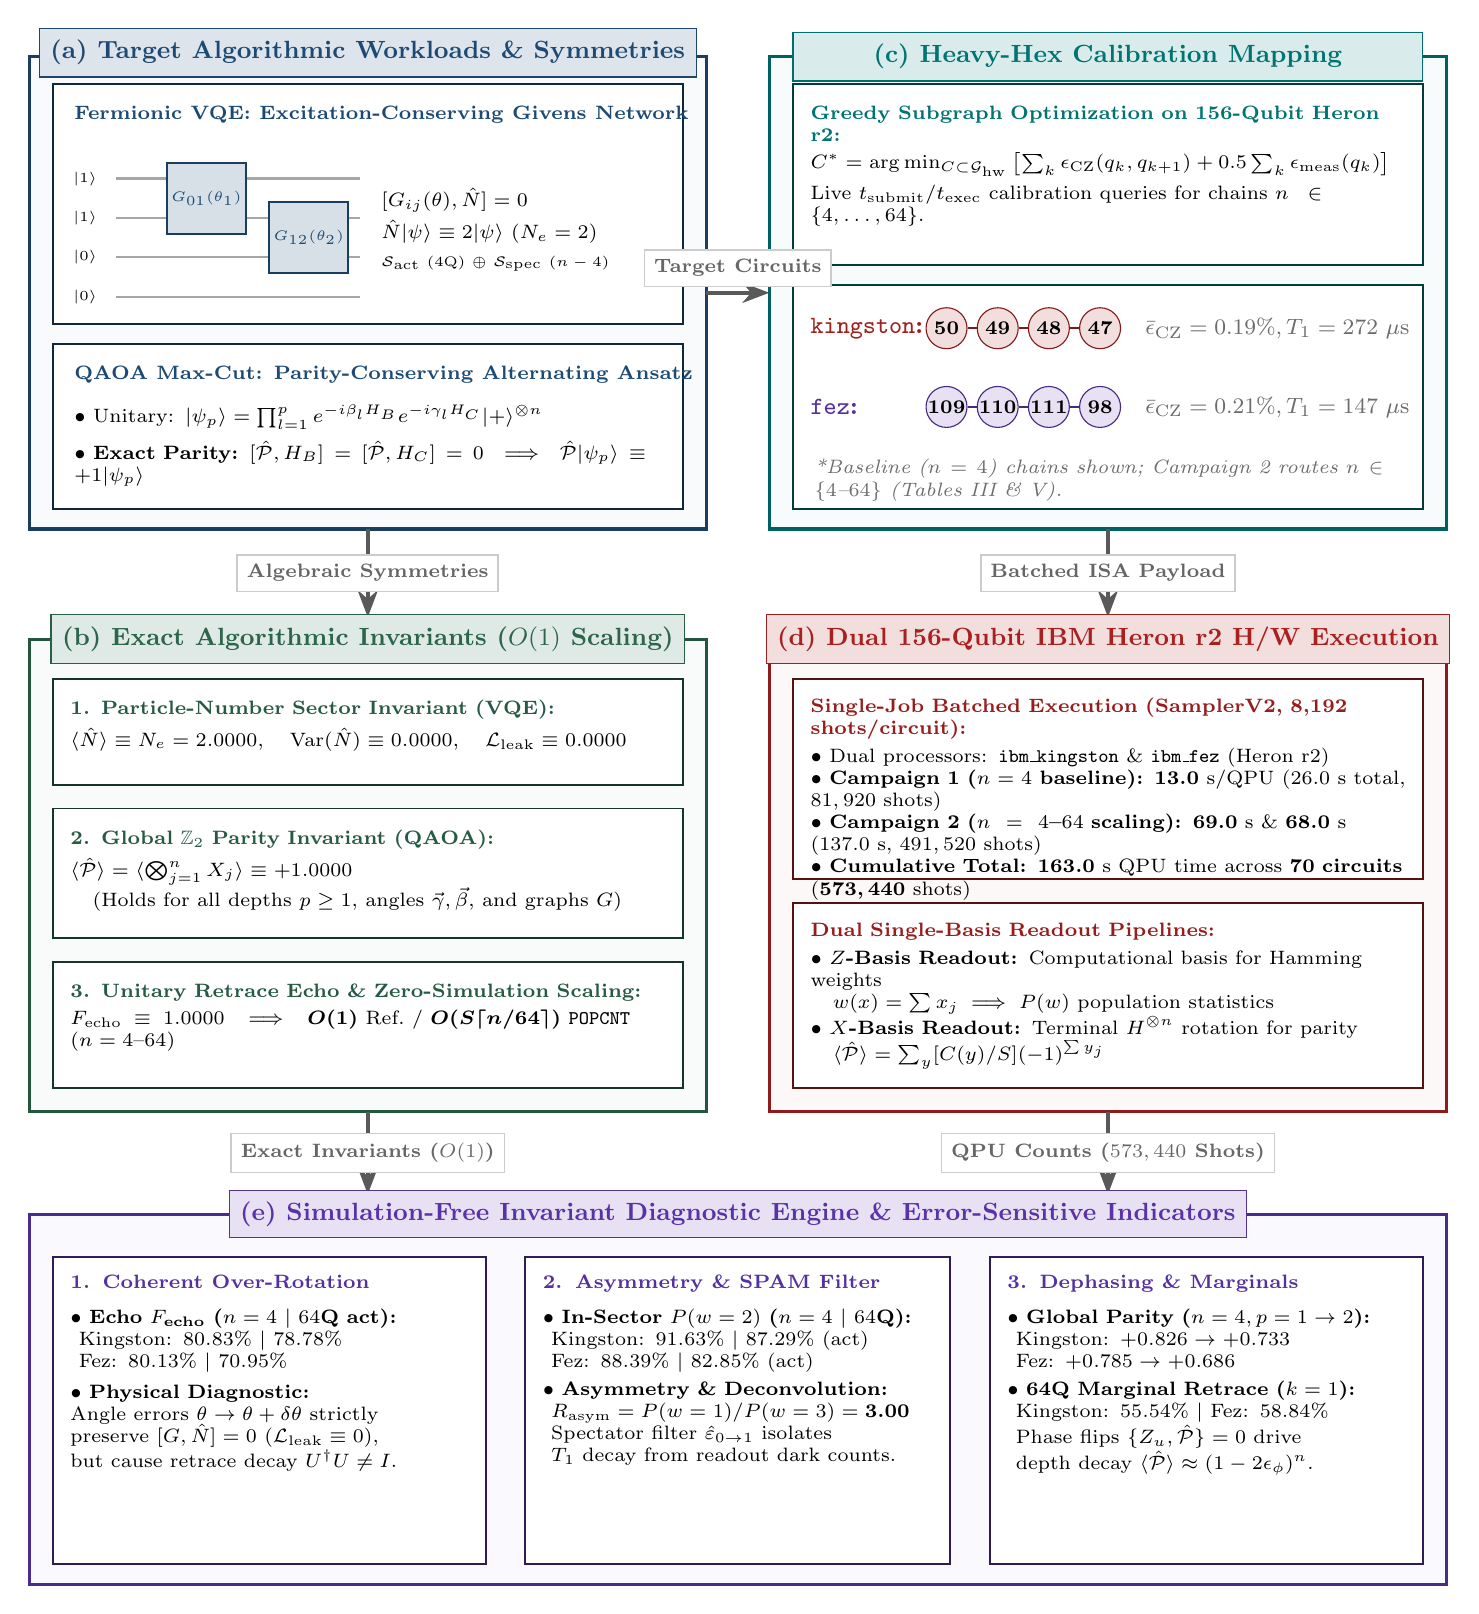
\begin{tikzpicture}[
    >=Stealth,
    font=\small,
    panel/.style={
        draw=#1!80!black, fill=#1!3, line width=1.1pt
    },
    titlepill/.style={
        draw=#1!90!black, fill=#1!15,
        font=\small\bfseries, text=#1!95!black, inner sep=4pt
    },
    cardheader/.style={
        draw=#1!90!black, fill=#1!15,
        font=\small\bfseries, text=#1!95!black, inner sep=4pt,
        minimum width=8.0cm, minimum height=0.62cm, align=center
    },
    innercard/.style={
        draw=#1!50!black, fill=white, line width=0.7pt,
        inner sep=5pt
    },
    pipe/.style={
        ->, line width=1.5pt, color=gray!70!black
    },
    pipetag/.style={
        fill=white, inner sep=3.5pt, font=\scriptsize\bfseries, text=gray!80!black, draw=gray!40, line width=0.6pt
    },
    qubit/.style={
        circle, draw=#1!75!black, fill=#1!15,
        minimum size=0.52cm, inner sep=0pt,
        font=\scriptsize\bfseries
    }
]

% ==============================================================================
% TOP TIER: (a) Workloads & (c) Mapping (y in [13.4, 19.4], height = 6.0cm)
% ==============================================================================

% Panel (a): Target Algorithms (x in [0, 8.6], y in [13.4, 19.4]) - Header length/height equal to d
\draw[panel=apsblue] (0, 13.4) rectangle (8.6, 19.4);
\node[cardheader=apsblue] at (4.3, 19.45) {(a) Target Algorithmic Workloads \& Symmetries};

% VQE Circuit sub-card (Generous height, title strictly separated from circuit)
\draw[innercard=apsblue] (0.3, 16.00) rectangle (8.3, 19.05);
\node[anchor=north west, font=\scriptsize\bfseries, text=apsblue!95!black] at (0.45, 18.90) {Fermionic VQE: Excitation-Conserving Givens Network};

% Quantum rails (Starting at x=1.1, keeping state labels safely inside x=0.3)
\draw[thick, gray!70] (1.1, 17.85) node[left=3pt, font=\tiny\bfseries, text=black] {$|1\rangle$} -- (4.2, 17.85);
\draw[thick, gray!70] (1.1, 17.35) node[left=3pt, font=\tiny\bfseries, text=black] {$|1\rangle$} -- (4.2, 17.35);
\draw[thick, gray!70] (1.1, 16.85) node[left=3pt, font=\tiny\bfseries, text=black] {$|0\rangle$} -- (4.2, 16.85);
\draw[thick, gray!70] (1.1, 16.35) node[left=3pt, font=\tiny\bfseries, text=black] {$|0\rangle$} -- (4.2, 16.35);

% Gate G01 (Sharp rectangular gate, comfortably 0.55cm below title)
\draw[draw=apsblue!80!black, fill=apsblue!18, line width=0.8pt] (1.75, 17.15) rectangle (2.75, 18.05);
\node[font=\tiny\bfseries, text=apsblue!95!black] at (2.25, 17.60) {$G_{01}(\theta_1)$};

% Gate G12 (Sharp rectangular gate)
\draw[draw=apsblue!80!black, fill=apsblue!18, line width=0.8pt] (3.05, 16.65) rectangle (4.05, 17.55);
\node[font=\tiny\bfseries, text=apsblue!95!black] at (3.55, 17.10) {$G_{12}(\theta_2)$};

% Lie symmetry label (Cleanly placed to the right of gates)
\node[anchor=west, font=\scriptsize, align=left] at (4.35, 17.20) {
    $[G_{ij}(\theta), \hat{N}] = 0$\\[2pt]
    $\hat{N}|\psi\rangle \equiv 2 |\psi\rangle$ ($N_e = 2$)\\[2pt]
    {\tiny $\mathcal{S}_{\text{act}}$ ($4\text{Q}$) $\oplus$ $\mathcal{S}_{\text{spec}}$ ($n-4$)}
};

% QAOA sub-card (Sharp corners)
\draw[innercard=apsblue] (0.3, 13.65) rectangle (8.3, 15.75);
\node[anchor=north west, font=\scriptsize\bfseries, text=apsblue!95!black] at (0.45, 15.60) {QAOA Max-Cut: Parity-Conserving Alternating Ansatz};
\node[anchor=north west, font=\scriptsize, align=left, text width=7.6cm] at (0.45, 15.10) {
    $\bullet$ Unitary: $|\psi_p\rangle = \prod_{l=1}^p e^{-i\beta_l H_B} e^{-i\gamma_l H_C} |+\rangle^{\otimes n}$\\[3pt]
    $\bullet$ \textbf{Exact Parity:} $[\hat{\mathcal{P}}, H_B] = [\hat{\mathcal{P}}, H_C] = 0 \implies \hat{\mathcal{P}}|\psi_p\rangle \equiv +1|\psi_p\rangle$
};


% Panel (c): Calibration Mapping (x in [9.4, 18.0], y in [13.4, 19.4]) - Header length/height equal to d
\draw[panel=apsteal] (9.4, 13.4) rectangle (18.0, 19.4);
\node[cardheader=apsteal] at (13.7, 19.4) {(c) Heavy-Hex Calibration Mapping};

\draw[innercard=apsteal] (9.7, 16.75) rectangle (17.7, 19.05);
\node[anchor=north west, font=\scriptsize, align=left, text width=7.6cm] at (9.8, 18.90) {
    \textbf{\textcolor{apsteal!95!black}{Greedy Subgraph Optimization on 156-Qubit Heron r2:}}\\[2pt]
    $C^* = \arg\min_{C \subset \mathcal{G}_{\text{hw}}} \left[ \sum_{k} \epsilon_{\text{CZ}}(q_k, q_{k+1}) + 0.5 \sum_{k} \epsilon_{\text{meas}}(q_k) \right]$\\[2pt]
    Live $t_{\text{submit}} / t_{\text{exec}}$ calibration queries for chains $n \in \{4, \dots, 64\}$.
};

% Qubit topology diagram (With footnote clarifying Campaign 1 n=4 vs Campaign 2 n=4..64)
\draw[innercard=apsteal] (9.7, 13.65) rectangle (17.7, 16.50);
% Kingston
\node[anchor=west, font=\small\bfseries, text=apsred!90!black] at (9.80, 15.95) {\texttt{kingston}:};
\node[qubit=apsred] (k50) at (11.65, 15.95) {50};
\node[qubit=apsred] (k49) at (12.30, 15.95) {49};
\node[qubit=apsred] (k48) at (12.95, 15.95) {48};
\node[qubit=apsred] (k47) at (13.60, 15.95) {47};
\draw[thick, apsred!75!black] (k50) -- (k49) -- (k48) -- (k47);
\node[anchor=west, font=\footnotesize, text=gray!85!black] at (14.05, 15.95) {$\bar{\epsilon}_{\text{CZ}}=0.19\%, T_1=272\ \mu\text{s}$};

% Fez
\node[anchor=west, font=\small\bfseries, text=apspurple!90!black] at (9.80, 14.95) {\texttt{fez}:};
\node[qubit=apspurple] (f109) at (11.65, 14.95) {109};
\node[qubit=apspurple] (f110) at (12.30, 14.95) {110};
\node[qubit=apspurple] (f111) at (12.95, 14.95) {111};
\node[qubit=apspurple] (f98)  at (13.60, 14.95) {98};
\draw[thick, apspurple!75!black] (f109) -- (f110) -- (f111) -- (f98);
\node[anchor=west, font=\footnotesize, text=gray!85!black] at (14.05, 14.95) {$\bar{\epsilon}_{\text{CZ}}=0.21\%, T_1=147\ \mu\text{s}$};

% Footnote inside Panel (c) sub-card (strictly bounded within 7.5cm width)
\node[anchor=west, font=\scriptsize\itshape, text=gray!85!black, text width=7.5cm] at (9.85, 14.02) {*Baseline ($n=4$) chains shown; Campaign 2 routes $n \in \{4\text{--}64\}$ (Tables~III \& V).};


% ==============================================================================
% TOP-TO-MIDDLE VERTICAL PIPES (Shortened by 30% -> 1.4cm corridor)
% ==============================================================================

% Left: (a) -> (b) with centered pipetag badge
\draw[pipe] (4.3, 13.4) -- node[pipetag] {Algebraic Symmetries} (4.3, 12.28);

% Right: (c) -> (d) with centered pipetag badge
\draw[pipe] (13.7, 13.4) -- node[pipetag] {Batched ISA Payload} (13.7, 12.28);

% Horizontal: (a) -> (c) across top
\draw[pipe] (8.6, 16.4) -- node[pipetag, above=2pt] {Target Circuits} (9.4, 16.4);


% ==============================================================================
% MIDDLE TIER: (b) Invariants & (d) Hardware Execution (y in [6.0, 12.0], height = 6.0cm)
% ==============================================================================

% Panel (b): Exact Invariants (x in [0, 8.6], y in [6.0, 12.0]) - Header length/height equal to d
\draw[panel=apsgreen] (0, 6.0) rectangle (8.6, 12.0);
\node[cardheader=apsgreen] at (4.3, 12.0) {(b) Exact Algorithmic Invariants ($O(1)$ Scaling)};

% Invariant 1: Fock
\draw[innercard=apsgreen] (0.3, 10.15) rectangle (8.3, 11.50);
\node[anchor=north west, font=\scriptsize, align=left, text width=7.6cm] at (0.4, 11.35) {
    \textbf{\textcolor{apsgreen!85!black}{1. Particle-Number Sector Invariant (VQE):}}\\[2pt]
    $\langle \hat{N} \rangle \equiv N_e = 2.0000, \quad \text{Var}(\hat{N}) \equiv 0.0000, \quad \mathcal{L}_{\text{leak}} \equiv 0.0000$
};

% Invariant 2: Parity
\draw[innercard=apsgreen] (0.3, 8.20) rectangle (8.3, 9.85);
\node[anchor=north west, font=\scriptsize, align=left, text width=7.6cm] at (0.4, 9.70) {
    \textbf{\textcolor{apsgreen!85!black}{2. Global $\mathbb{Z}_2$ Parity Invariant (QAOA):}}\\[2pt]
    $\langle \hat{\mathcal{P}} \rangle = \langle \bigotimes_{j=1}^n X_j \rangle \equiv +1.0000$\\
    \hspace*{8pt}(Holds for all depths $p \ge 1$, angles $\vec{\gamma}, \vec{\beta}$, and graphs $G$)
};

% Invariant 3: Retrace Echo & Scaling
\draw[innercard=apsgreen] (0.3, 6.30) rectangle (8.3, 7.90);
\node[anchor=north west, font=\scriptsize, align=left, text width=7.6cm] at (0.4, 7.75) {
    \textbf{\textcolor{apsgreen!85!black}{3. Unitary Retrace Echo \& Zero-Simulation Scaling:}}\\[2pt]
    $F_{\text{echo}} \equiv 1.0000 \implies \bm{O(1)}$ Ref.\ / $\bm{O(S\lceil n/64\rceil)}$ \texttt{POPCNT} ($n=4\text{--}64$)
};


% Panel (d): Hardware Execution (x in [9.4, 18.0], y in [6.0, 12.0]) - Benchmark standard header
\draw[panel=apsred] (9.4, 6.0) rectangle (18.0, 12.0);
\node[cardheader=apsred] at (13.7, 12.0) {(d) Dual 156-Qubit IBM Heron r2 H/W Execution};

\draw[innercard=apsred] (9.7, 8.95) rectangle (17.7, 11.50);
\node[anchor=north west, font=\scriptsize, align=left, text width=7.6cm] at (9.8, 11.38) {
    \textbf{\textcolor{apsred!85!black}{Single-Job Batched Execution (SamplerV2, 8,192 shots/circuit):}}\\[2pt]
    $\bullet$ Dual processors: \texttt{ibm\_kingston} \& \texttt{ibm\_fez} (Heron r2)\\
    $\bullet$ \textbf{Campaign 1 ($n=4$ baseline):} $\bm{13.0\text{ s}}$/QPU ($26.0\text{ s}$ total, $81,920$ shots)\\
    $\bullet$ \textbf{Campaign 2 ($n=4\text{--}64$ scaling):} $\bm{69.0\text{ s}}$ \& $\bm{68.0\text{ s}}$ ($137.0\text{ s}$, $491,520$ shots)\\
    $\bullet$ \textbf{Cumulative Total:} $\bm{163.0\text{ s}}$ QPU time across \textbf{70 circuits} ($\bm{573,440}$ shots)
};

\draw[innercard=apsred] (9.7, 6.30) rectangle (17.7, 8.65);
\node[anchor=north west, font=\scriptsize, align=left, text width=7.6cm] at (9.8, 8.52) {
    \textbf{\textcolor{apsred!85!black}{Dual Single-Basis Readout Pipelines:}}\\[2pt]
    $\bullet$ \textbf{$Z$-Basis Readout:} Computational basis for Hamming weights\\
    \hspace*{8pt}$w(x) = \sum x_j \implies P(w)$ population statistics\\
    $\bullet$ \textbf{$X$-Basis Readout:} Terminal $H^{\otimes n}$ rotation for parity\\
    \hspace*{8pt}$\langle \hat{\mathcal{P}} \rangle = \sum_y [C(y)/S] (-1)^{\sum y_j}$
};


% ==============================================================================
% MIDDLE-TO-BOTTOM VERTICAL PIPES (Shortened corridor)
% ==============================================================================

% Left: (b) -> (e) with centered pipetag badge
\draw[pipe] (4.3, 6.0) -- node[pipetag] {Exact Invariants ($O(1)$)} (4.3, 4.95);

% Right: (d) -> (e) with centered pipetag badge
\draw[pipe] (13.7, 6.0) -- node[pipetag] {QPU Counts ($573,440$ Shots)} (13.7, 4.95);


% ==============================================================================
% BOTTOM TIER: (e) Invariant Diagnostic Engine (y in [0.0, 4.7], height = 4.7cm)
% ==============================================================================

% Panel (e)
\draw[panel=apspurple] (0, 0.0) rectangle (18.0, 4.7);
\node[titlepill=apspurple] at (9.0, 4.7) {(e) Simulation-Free Invariant Diagnostic Engine \& Error-Sensitive Indicators};

% Card E1: Coherent Gate Miscalibration (Sharp corners)
\draw[innercard=apspurple] (0.3, 0.25) rectangle (5.8, 4.15);
\node[anchor=north west, font=\scriptsize\bfseries, text=apspurple!90!black, text width=5.1cm] at (0.4, 4.05) {1. Coherent Over-Rotation};
\node[anchor=north west, font=\scriptsize, align=left, text width=5.1cm] at (0.4, 3.62) {
    $\bullet$ \textbf{Echo $F_{\text{echo}}$ ($n=4$ $|$ $64\text{Q}$ act):}\\
    \hspace*{3pt}Kingston: $80.83\%$ $|$ $78.78\%$\\
    \hspace*{3pt}Fez: $80.13\%$ $|$ $70.95\%$\\[3pt]
    $\bullet$ \textbf{Physical Diagnostic:}\\
    Angle errors $\theta \to \theta + \delta\theta$ strictly\\
    preserve $[G, \hat{N}] = 0$ ($\mathcal{L}_{\text{leak}} \equiv 0$),\\
    but cause retrace decay $U^\dagger U \neq I$.
};

% Card E2: Directional Population Asymmetry & SPAM Filter
\draw[innercard=apspurple] (6.3, 0.25) rectangle (11.7, 4.15);
\node[anchor=north west, font=\scriptsize\bfseries, text=apspurple!90!black, text width=5.0cm] at (6.4, 4.05) {2. Asymmetry \& SPAM Filter};
\node[anchor=north west, font=\scriptsize, align=left, text width=5.0cm] at (6.4, 3.62) {
    $\bullet$ \textbf{In-Sector $P(w=2)$ ($n=4$ $|$ $64\text{Q}$):}\\
    \hspace*{3pt}Kingston: $91.63\%$ $|$ $87.29\%$ (act)\\
    \hspace*{3pt}Fez: $88.39\%$ $|$ $82.85\%$ (act)\\[2pt]
    $\bullet$ \textbf{Asymmetry \& Deconvolution:}\\
    \hspace*{3pt}$R_{\text{asym}} = P(w=1)/P(w=3) = \bm{3.00}$\\
    \hspace*{3pt}Spectator filter $\hat{\varepsilon}_{0\to 1}$ isolates\\
    \hspace*{3pt}$T_1$ decay from readout dark counts.
};

% Card E3: Multi-Qubit Dephasing & Local Marginals
\draw[innercard=apspurple] (12.2, 0.25) rectangle (17.7, 4.15);
\node[anchor=north west, font=\scriptsize\bfseries, text=apspurple!90!black, text width=5.1cm] at (12.3, 4.05) {3. Dephasing \& Marginals};
\node[anchor=north west, font=\scriptsize, align=left, text width=5.1cm] at (12.3, 3.62) {
    $\bullet$ \textbf{Global Parity ($n=4, p=1\to 2$):}\\
    \hspace*{3pt}Kingston: $+0.826 \to +0.733$\\
    \hspace*{3pt}Fez: $+0.785 \to +0.686$\\[2pt]
    $\bullet$ \textbf{64Q Marginal Retrace ($k=1$):}\\
    \hspace*{3pt}Kingston: $55.54\%$ $|$ Fez: $58.84\%$\\
    \hspace*{3pt}Phase flips $\{Z_u, \hat{\mathcal{P}}\} = 0$ drive\\
    \hspace*{3pt}depth decay $\langle \hat{\mathcal{P}} \rangle \approx (1 - 2\epsilon_\phi)^n$.
};

\end{tikzpicture}%
}
\caption{\textbf{AlgoInvar Architectural Workflow and Simulation-Free Diagnostic Engine.} (a) Target variational algorithms in fermionic chemistry (excitation-conserving Givens networks) and Max-Cut optimization (QAOA alternating ansatz) govern exact Lie and $\mathbb{Z}_2$ parity symmetries. (b) Exact parameter-free invariants ($\langle \hat{N} \rangle \equiv N_e$, $\text{Var}(\hat{N}) \equiv 0$, $\mathcal{L}_{\text{leak}} \equiv 0$, $\langle \hat{\mathcal{P}} \rangle \equiv +1.0$, $F_{\text{echo}} \equiv 1.0$) establish analytical verification baselines with zero classical simulation ($O(1)$ theoretical reference complexity with linear $O(S \cdot n)$ bitstring post-processing at arbitrary $n$). (c) Calibration-guided subgraph search isolates optimal connected physical chains of width $n \in \{4, 8, 12, 16, 32, 64\}$ on 156-qubit IBM Heron r2 backends (shown for the baseline $n = 4$ campaign on \texttt{ibm\_kingston}: $[50,49,48,47]$ and \texttt{ibm\_fez}: $[109,110,111,98]$). (d) Single-job batching submits circuits simultaneously ($8,192$ shots per circuit; $40,960$ shots in $13.0$~s QPU time for the $n = 4$ baseline campaign, and $245,760$ shots across $30$ circuits in $68.0$--$69.0$~s QPU time for the $n = 4 \to 64$ scaling campaign). (e) Empirical single-basis readouts yield phenomenological diagnostic proxies that differentiate coherent gate over-rotations from directional population asymmetry ($R_{\text{asym}} = 3.00 \pm 0.24$ on \texttt{ibm\_fez}) consistent with preferential relaxation and readout bias and multi-qubit entangling dephasing across circuit depth $p$. Empirical estimates carry binomial sampling uncertainties $\sigma = \sqrt{P(1-P)/S}$.}
\label{fig:methodology}
\end{figure*}

% ==============================================================================
% SECTION II: THEORETICAL FOUNDATIONS
% ==============================================================================
\section{Theoretical Foundations}
The overarching architectural workflow of AlgoInvar, spanning algorithmic state preparation, exact analytical invariance, calibration-guided qubit routing, and single-basis diagnostic readouts, is illustrated in Figure~\ref{fig:methodology}. The mathematical invariants formulated in AlgoInvar, along with their conserved observables, commutation relations, and physical error signatures, are summarized in Table~\ref{tab:invariants}.

\subsection{Particle-Number Sector Conservation in VQE}
In quantum electronic structure problems mapped to qubits via the Jordan--Wigner transformation~\cite{Jordan1928, Ortiz2001}, fermionic creation and annihilation operators $a_j^\dagger, a_j$ map to non-local Pauli strings:
\begin{equation}
a_j^\dagger = \left( \bigotimes_{k < j} Z_k \right) \frac{X_j - i Y_j}{2}, \quad a_j = \left( \bigotimes_{k < j} Z_k \right) \frac{X_j + i Y_j}{2}.
\end{equation}
The total particle number operator $\hat{N} = \sum_{j=1}^n a_j^\dagger a_j$ translates directly into a diagonal sum of single-qubit Pauli-$Z$ operators:
\begin{equation}
\hat{N} = \sum_{j=1}^n \frac{I - Z_j}{2}.
\label{eq:number_op}
\end{equation}

In conservative quantum chemical systems with $N_e$ electrons, the electronic Hamiltonian commutes with particle number: $[\hat{H}_e, \hat{N}] = 0$. Symmetry-adapted variational circuits, such as particle-conserving Givens rotation networks [Figure~\ref{fig:methodology}(a,b)], restrict state evolution strictly to the $N_e$-particle Fock subspace~\cite{Barkoutsos2018, Wecker2015}.

A two-qubit Givens rotation gate $G_{ij}(\theta)$ acting on adjacent qubits $i$ and $j$ is generated by the planar excitation Hamiltonian:
\begin{equation}
G_{ij}(\theta) = \exp\left[ -i \frac{\theta}{4} (X_i X_j + Y_i Y_j) \right].
\end{equation}
In the computational basis $\{|00\rangle, |01\rangle, |10\rangle, |11\rangle\}$, $G_{ij}(\theta)$ evaluates to:
\begin{equation}
G_{ij}(\theta) = \begin{pmatrix}
1 & 0 & 0 & 0 \\
0 & \cos\frac{\theta}{2} & -i\sin\frac{\theta}{2} & 0 \\
0 & -i\sin\frac{\theta}{2} & \cos\frac{\theta}{2} & 0 \\
0 & 0 & 0 & 1
\end{pmatrix}.
\end{equation}
Specifically, $G_{ij}(\theta)$ acts as a unitary transformation solely within the single-excitation subspace $\{|01\rangle, |10\rangle\}$, leaving $|00\rangle$ and $|11\rangle$ invariant.

\textbf{Theorem 1 (Particle-Number Sector Invariant):} 
Let $U_{\text{VQE}}(\vec{\theta}) = \prod_{k=1}^M G_{i_k j_k}(\theta_k)$ be an arbitrary-depth network of Givens rotations. For any initial state $|\psi_0\rangle$ with definite particle number $N_e$ (i.e., $\hat{N}|\psi_0\rangle = N_e |\psi_0\rangle$), the state $|\psi(\vec{\theta})\rangle = U_{\text{VQE}}(\vec{\theta})|\psi_0\rangle$ satisfies:
\begin{align}
\langle \hat{N} \rangle &\equiv \langle \psi(\vec{\theta}) | \hat{N} | \psi(\vec{\theta}) \rangle = N_e \quad \forall \vec{\theta} \in \mathbb{R}^M, \label{eq:inv_mean} \\
\text{Var}(\hat{N}) &\equiv \langle \hat{N}^2 \rangle - \langle \hat{N} \rangle^2 = 0 \quad \forall \vec{\theta} \in \mathbb{R}^M. \label{eq:inv_var}
\end{align}

\emph{Proof.} Direct calculation of the commutator between the two-body generator and the local number operators on qubits $i$ and $j$ yields:
\begin{align}
[X_i X_j + Y_i Y_j, Z_i + Z_j] &= [X_i X_j, Z_i] + [X_i X_j, Z_j] \nonumber \\
&\quad + [Y_i Y_j, Z_i] + [Y_i Y_j, Z_j] \nonumber \\
&= -2i Y_i X_j - 2i X_i Y_j \nonumber \\
&\quad + 2i X_i Y_j + 2i Y_i X_j \nonumber \\
&= 0.
\end{align}
Because $\hat{N} = \frac{n}{2} I - \frac{1}{2}\sum_{k=1}^n Z_k$, and all spectator terms $Z_k$ ($k \neq i, j$) commute with $G_{ij}(\theta)$, it follows that $[G_{ij}(\theta), \hat{N}] = 0$ for all $i, j, \theta$. Consequently, $[U_{\text{VQE}}(\vec{\theta}), \hat{N}] = 0$. Hence:
\begin{equation}
\hat{N} |\psi(\vec{\theta})\rangle = U_{\text{VQE}}(\vec{\theta}) \hat{N} |\psi_0\rangle = N_e |\psi(\vec{\theta})\rangle,
\end{equation}
establishing that $|\psi(\vec{\theta})\rangle$ remains an exact eigenstate of $\hat{N}$ with eigenvalue $N_e$, proving Eqs.~\eqref{eq:inv_mean} and~\eqref{eq:inv_var}. \hfill $\square$

\textbf{Measurement Protocol:} Evaluating $\langle \hat{N} \rangle$ and $\text{Var}(\hat{N})$ requires no multi-basis tomography. In the computational $Z$-basis, every measured bitstring $x = (x_1, \dots, x_n) \in \{0, 1\}^n$ is an eigenstate of $\hat{N}$ with eigenvalue equal to its Hamming weight:
\begin{equation}
\text{wt}(x) = \sum_{j=1}^n x_j.
\end{equation}
Given experimental counts $C(x)$ over total shots $S = \sum_x C(x)$, the sample moments are computed directly:
\begin{equation}
\langle \hat{N} \rangle = \sum_x \frac{C(x)}{S} \text{wt}(x), \quad \langle \hat{N}^2 \rangle = \sum_x \frac{C(x)}{S} [\text{wt}(x)]^2.
\end{equation}
In our software implementation (\texttt{cpp/}), bitstring Hamming weights $\text{wt}(x)$ and $X$-basis parity eigenvalues $(-1)^{\sum y_j}$ across wide registers ($n \le 156$) are evaluated in $O(S \cdot \lceil n/64 \rceil)$ time using 64-bit hardware population-count (\texttt{POPCNT}) CPU intrinsics in C++17 (\texttt{\_\_popcnt64} and \texttt{\_\_builtin\_popcountll}) exposed to Python via \texttt{pybind11}, performing strictly classical bitstring counting with zero quantum statevector simulation. We define the \emph{particle-number-sector leakage} (or \emph{out-of-sector population}) $\mathcal{L}_{\text{leak}}$ as the total measured probability mass outside the target $N_e$-particle Hamming-weight sector:
\begin{equation}
\mathcal{L}_{\text{leak}} = 1 - \sum_{x:\,\text{wt}(x) = N_e} \frac{C(x)}{S}.
\label{eq:leakage}
\end{equation}
We emphasize that $\mathcal{L}_{\text{leak}}$ quantifies population scattering outside the intended computational excitation subspace (here $w = N_e = 2$ within $\{0,1\}^n$) arising from gate infidelities, incoherent dissipation, and readout assignment errors. It is conceptually and physically distinct from transmon leakage out of the computational qubit manifold into non-computational transmon energy levels (such as $|2\rangle$ or $|3\rangle$), which requires dedicated spectroscopic multi-state discrimination sweeps.

Furthermore, we highlight that pure computational-basis dephasing ($Z$) commutes identically with the diagonal number operator: $[\hat{N}, Z_k] = 0$. Consequently, while pure phase dephasing dampens off-diagonal coherences between distinct computational states within the $N_e = 2$ manifold, it leaves the diagonal population distribution $P(w)$ invariant and does not, by itself, generate non-zero particle variance or out-of-sector population. Non-zero measured variance ($\text{Var}(\hat{N}) > 0$) and leakage ($\mathcal{L}_{\text{leak}} > 0$) are strictly driven by excitation-non-conserving processes: longitudinal thermal relaxation, non-excitation-preserving gate errors, and classical detector assignment errors.

% TABLE I: THEORETICAL INVARIANTS SUMMARY
\begin{table*}[t]
\caption{\label{tab:invariants}\textbf{Theoretical Invariant Formulations in AlgoInvar.} Conserved observables, algebraic commutation relations, exact analytical reference values, and phenomenological physical error signatures diagnosed by each invariant. Empirical invariant estimates from $S$ shots carry standard binomial sampling uncertainties $\sigma = \sqrt{P(1-P)/S}$, which scale as $O(1/\sqrt{S})$. For $S = 8,192$, standard errors range from $\pm 0.003$ to $\pm 0.008$.}
\begin{tabular*}{\textwidth}{@{\extracolsep{\fill}} p{3cm} c c c c p{4.6cm}}
\hline\hline
\textbf{Benchmark /} & \textbf{Target} & \textbf{Conserved} & \textbf{Commutation} & \textbf{Exact} & \textbf{Diagnosed Physical} \\
\textbf{Invariant} & \textbf{Workload} & \textbf{Observable $\hat{\mathcal{O}}$} & \textbf{Symmetry} & \textbf{Value} & \textbf{Error Signature} \\
\hline
\shortstack[l]{Particle Expectation\\$\langle \hat{N} \rangle$} & VQE Chemistry & $\sum_j \frac{I-Z_j}{2}$ & $[\hat{N}, G_{ij}(\theta)] = 0$ & $N_e = 2.0000$ & Phenomenological indicator of thermal relaxation ($T_1$) asymmetry ($\langle \hat{N} \rangle < N_e$) and dissipative decay \\
\hline
\shortstack[l]{Particle Variance\\$\text{Var}(\hat{N})$} & VQE Chemistry & $(\hat{N} - \langle \hat{N} \rangle)^2$ & $[\hat{N}^2, G_{ij}(\theta)] = 0$ & $0.0000$ & Excitation-changing gate infidelities, amplitude damping, and SPAM error \\
\hline
\shortstack[l]{Out-of-Sector Leakage\\$\mathcal{L}_{\text{leak}}$} & VQE Chemistry & $\sum_{w \neq N_e} P(w)$ & Excitation projection & $0.0000$ & Incoherent dissipation, excitation-changing errors, and SPAM assignment \\
\hline
\shortstack[l]{VQE Echo Fidelity\\$F_{\text{echo}}$} & VQE Retrace & $|\psi_0\rangle \langle \psi_0|$ & $U^\dagger(\vec{\theta}) U(\vec{\theta}) = I$ & $1.0000$ & Coherent rotation overshoots and pulse envelope miscalibrations \\
\hline
\shortstack[l]{Global Parity\\$\langle \hat{\mathcal{P}} \rangle$} & QAOA Max-Cut & $\bigotimes_{j=1}^n X_j$ & $[\hat{\mathcal{P}}, H_B] = [\hat{\mathcal{P}}, H_C] = 0$ & $+1.0000$ & Multi-qubit entangling gate crosstalk and phase dephasing accumulation \\
\hline
\shortstack[l]{QAOA Echo Fidelity\\$F_{\text{echo}}$} & QAOA Retrace & $|+\rangle^{\otimes n} \langle +|^{\otimes n}$ & $U_{\text{QAOA}}^\dagger U_{\text{QAOA}} = I$ & $1.0000$ & Depth-dependent entangling error accumulation across layers $p$ \\
\hline\hline
\end{tabular*}
\end{table*}

\subsection{Global \texorpdfstring{$\mathbb{Z}_2$}{Z2} Parity Invariance in QAOA}
In QAOA applied to graph partitioning problems such as Max-Cut on an undirected graph $G = (V, E)$ with $|V| = n$ vertices~\cite{Farhi2014, Hadfield2019, Zhou2020, Bapat2019}, the cost Hamiltonian is:
\begin{equation}
H_C = \frac{1}{2} \sum_{(u, v) \in E} (I - Z_u Z_v).
\end{equation}
The standard mixer Hamiltonian is the transverse-field operator:
\begin{equation}
H_B = \sum_{u \in V} X_u.
\end{equation}
Starting from the symmetric uniform superposition $|+\rangle^{\otimes n}$, the depth-$p$ QAOA state is prepared via alternating unitaries:
\begin{equation}
|\psi_p(\vec{\gamma}, \vec{\beta})\rangle = \prod_{l=1}^p \left( e^{-i \beta_l H_B} e^{-i \gamma_l H_C} \right) |+\rangle^{\otimes n}.
\end{equation}

We define the global parity operator across all $n$ qubits as the collective $X$-spin:
\begin{equation}
\hat{\mathcal{P}} = \bigotimes_{u \in V} X_u.
\label{eq:parity_op}
\end{equation}

\textbf{Theorem 2 (Global QAOA Parity Invariant):} 
For any graph $G = (V, E)$, any depth $p \ge 1$, and arbitrary parameter schedules $(\vec{\gamma}, \vec{\beta}) \in \mathbb{R}^{2p}$, the global parity expectation value satisfies:
\begin{equation}
\langle \hat{\mathcal{P}} \rangle \equiv \langle \psi_p(\vec{\gamma}, \vec{\beta}) | \hat{\mathcal{P}} | \psi_p(\vec{\gamma}, \vec{\beta}) \rangle = +1.0.
\label{eq:qaoa_invariant}
\end{equation}

\emph{Proof.} First, evaluate the action of $\hat{\mathcal{P}}$ on the initial state $|+\rangle^{\otimes n}$. Because $X|+\rangle = |+\rangle$, we have $\hat{\mathcal{P}} |+\rangle^{\otimes n} = |+\rangle^{\otimes n}$.
Second, examine the commutation relations with the generators $H_B$ and $H_C$:
\begin{equation}
[\hat{\mathcal{P}}, H_B] = \left[ \bigotimes_{u} X_u, \sum_v X_v \right] = 0,
\end{equation}
since every single-qubit operator $X_v$ commutes with itself and acts trivially on all other sites.
For the cost Hamiltonian, every edge term is $Z_u Z_v$. Computing the commutator:
\begin{align}
\hat{\mathcal{P}} (Z_u Z_v) \hat{\mathcal{P}}^\dagger &= (X_u Z_u X_u) (X_v Z_v X_v) \left( \bigotimes_{w \neq u, v} X_w X_w \right) \nonumber \\
&= (-Z_u) (-Z_v) I = Z_u Z_v.
\end{align}
Thus $[\hat{\mathcal{P}}, Z_u Z_v] = 0$ for all $(u, v) \in E$, which implies $[\hat{\mathcal{P}}, H_C] = 0$.
Because $\hat{\mathcal{P}}$ commutes with both $H_B$ and $H_C$, it commutes with the entire compiled unitary:
\begin{equation}
[\hat{\mathcal{P}}, U_{\text{QAOA}}(\vec{\gamma}, \vec{\beta})] = 0.
\end{equation}
Therefore:
\begin{align}
\hat{\mathcal{P}} |\psi_p(\vec{\gamma}, \vec{\beta})\rangle &= U_{\text{QAOA}}(\vec{\gamma}, \vec{\beta}) \hat{\mathcal{P}} |+\rangle^{\otimes n} \nonumber \\
&= U_{\text{QAOA}}(\vec{\gamma}, \vec{\beta}) |+\rangle^{\otimes n} = |\psi_p(\vec{\gamma}, \vec{\beta})\rangle,
\end{align}
proving that $|\psi_p(\vec{\gamma}, \vec{\beta})\rangle$ is a strict $+1$ eigenstate of $\hat{\mathcal{P}}$, establishing Eq.~\eqref{eq:qaoa_invariant}. \hfill $\square$

\textbf{Measurement Protocol:} Measuring $\langle \hat{\mathcal{P}} \rangle$ requires rotating every qubit into the $X$-basis via a local Hadamard gate $H^{\otimes n}$ immediately prior to readout. If $y = (y_1, \dots, y_n) \in \{0, 1\}^n$ is the measured bitstring in the $X$-basis, the eigenvalue of $\hat{\mathcal{P}}$ is $(-1)^{\sum_j y_j}$. Given shot distribution $C(y)$:
\begin{equation}
\langle \hat{\mathcal{P}} \rangle = \sum_y \frac{C(y)}{S} (-1)^{\sum_j y_j}.
\end{equation}
Deviations of $\langle \hat{\mathcal{P}} \rangle$ from $+1.0$ selectively diagnose multi-qubit phase-type errors accumulated across all $p$ layers. Specifically, because $\hat{\mathcal{P}} = \bigotimes_{u \in V} X_u$, any Pauli-$Z$ error (and similarly Pauli-$Y$) anticommutes with $\hat{\mathcal{P}}$ ($\{Z_u, \hat{\mathcal{P}}\} = 0$), inverting the measured parity outcome. Conversely, Pauli-$X$ bit-flip errors commute with the parity operator ($[X_u, \hat{\mathcal{P}}] = 0$) and do not alter the parity eigenvalue. Therefore, QAOA parity invariance provides a targeted probe of phase dephasing and non-commuting generator infidelities, while remaining blind to pure $X$ errors.



\subsection{Unitary Retrace Echo Benchmarking}
To complement forward-circuit symmetry monitoring, AlgoInvar incorporates a unitary retrace echo protocol. Given a target unitary $U(\vec{\theta})$ (either the Givens VQE ansatz or the alternating QAOA sequence), the inverse circuit $U^\dagger(\vec{\theta})$ is compiled and executed immediately following $U(\vec{\theta})$.

For fermionic VQE on an $n$-qubit register ($n \ge 4$), state preparation begins from the reference two-electron Hartree-Fock computational state $|\psi_0\rangle = |110^{\otimes (n-2)}\rangle$ ($|1100\rangle$ at $n = 4$). The total round-trip sequence maps $|\psi_0\rangle \to U^\dagger(\vec{\theta}) U(\vec{\theta}) |\psi_0\rangle$. The echo return fidelity $F_{\text{echo}}$ is evaluated in the computational basis as the survival probability of the initial reference bitstring:
\begin{equation}
F_{\text{echo}}^{\text{VQE}} = \frac{C(|1100\rangle)}{S}.
\end{equation}
For QAOA, evolution begins from the equal superposition state $|+\rangle^{\otimes n}$. After appending $U_{\text{QAOA}}^\dagger(\vec{\gamma}, \vec{\beta})$, a terminal layer of local Hadamard gates rotates the state into the computational basis, where returning to $|+\rangle^{\otimes n}$ maps to measuring the all-zero state $|0^{\otimes n}\rangle$ ($|0000\rangle$ at $n = 4$):
\begin{equation}
F_{\text{echo}}^{\text{QAOA}} = \frac{C(|0000\rangle)}{S}.
\end{equation}

In an ideal, noiseless system, $U^\dagger U \equiv I$ identically, yielding $F_{\text{echo}} \equiv 1.0$ for all parameter angles. On noisy physical hardware, $F_{\text{echo}}$ decays due to accumulated gate infidelities, environmental decoherence ($T_1, T_2$), and coherent angle over-rotations. In our implementation, forward and inverse unitaries are transpiled through Qiskit's ISA transpiler without peephole cancellation of $U U^\dagger$. We note that while in-manifold coherent angle errors preserve particle number $\hat{N}$ strictly in the forward circuit ($\text{Var}(\hat{N}) \equiv 0$), echo fidelity reflects the cumulative effect of both coherent drifts and dissipative decay. Furthermore, if calibration errors are correlated between forward and inverse gates, partial coherent error cancellation can occur, potentially causing $F_{\text{echo}}$ to over-estimate circuit survival probabilities under systematic over-rotations. To decouple these symmetric echo-refocusing effects in practical characterization campaigns, the AlgoInvar framework can be natively paired with randomized compiling (RC) or Pauli twirling across the forward-inverse boundary~\cite{Wallman2016,Cai2019}. Interleaving random Pauli gates shifts systematic coherent accumulation into stochastic channels, ensuring that $F_{\text{echo}}$ reflects unmitigated structural drifts rather than accidental symmetric cancellation. Therefore, $F_{\text{echo}}$ serves as a composite benchmark of round-trip unitary preservation rather than an isolated coherent-error diagnostic.

\subsection{The AlgoInvar Benchmarking Protocol}
The operational execution of the AlgoInvar framework is summarized in Algorithm~\ref{alg:algoinvar}. The protocol requires zero classical statevector simulation, operating strictly via exact algebraic reference targets ($\langle \hat{N} \rangle \equiv N_e$, $\text{Var}(\hat{N}) \equiv 0$, and $\langle \hat{\mathcal{P}} \rangle \equiv +1$) and linear-time $O(S \cdot n)$ single-pass bitwise accumulation over $S$ measurement shots. By acquiring both forward and echo distributions and coupling in-sector confinement with directional asymmetry $R_{\text{asym}}$ and in situ spectator deconvolution, AlgoInvar simultaneously evaluates unitary gate preservation, isolates dissipative relaxation from spectator dark counts, and restores true active-manifold fidelity across utility-scale quantum processors.

\begin{algorithm}[H]
\caption{AlgoInvar In Situ Benchmarking and Diagnostic Protocol}
\label{alg:algoinvar}
\begin{algorithmic}[1]
\Require Hardware backend $\mathcal{Q}$, register width $n$, circuit class $\mathcal{C} \in \{\text{VQE}, \text{QAOA}\}$, parameter vector $\vec{\theta}$, shot budget $S$.
\Ensure Invariant observable $\langle \hat{\mathcal{I}} \rangle$, variance $\text{Var}(\hat{\mathcal{I}})$, echo fidelity $F_{\text{echo}}$, directional asymmetry ratio $R_{\text{asym}}$, and active-manifold fidelity $P_{\text{act}}$.
\Statex \textit{// 1. Dual-Branch Circuit Compilation}
\State Construct forward circuit $\mathcal{C}_{\text{fwd}} \gets U(\vec{\theta})$
\State Construct echo circuit $\mathcal{C}_{\text{echo}} \gets U^\dagger(\vec{\theta}) \mathcal{T} U(\vec{\theta})$ \Comment{$\mathcal{T} = I$ or Pauli twirling}
\Statex \textit{// 2. Physical Hardware Sampling}
\State Transpile $\mathcal{C}_{\text{fwd}}$ and $\mathcal{C}_{\text{echo}}$ to native ISA of $\mathcal{Q}$
\State Execute on $\mathcal{Q}$ with $S$ shots; acquire bitstrings $\mathcal{M}_{\text{fwd}}, \mathcal{M}_{\text{echo}} \subset \{0, 1\}^n$
\Statex \textit{// 3. Linear-Time Bitwise Post-Processing ($O(S \cdot n)$)}
\For{each measured bitstring $b^{(s)} \in \mathcal{M}_{\text{fwd}}$}
    \State Compute Hamming weight $w(b^{(s)}) \gets \sum_{j=1}^n b_j^{(s)}$
\EndFor
\If{$\mathcal{C} = \text{VQE}$} \Comment{Fermionic particle-number conservation}
    \State $\langle \hat{N} \rangle \gets \frac{1}{S}\sum_{s=1}^S w(b^{(s)})$
    \State $\text{Var}(\hat{N}) \gets \frac{1}{S}\sum_{s=1}^S (w(b^{(s)}) - \langle \hat{N} \rangle)^2$
    \State $P(w = N_e) \gets \frac{1}{S} \sum_{s=1}^S \mathbb{I}[w(b^{(s)}) = N_e]$
    \State $R_{\text{asym}} \gets \frac{\sum_{s} \mathbb{I}[w(b^{(s)}) < N_e]}{\sum_{s} \mathbb{I}[w(b^{(s)}) > N_e]}$ \Comment{$T_1$ loss vs.\ heating/crosstalk}
    \State $F_{\text{echo}} \gets \frac{1}{S}\sum_{s=1}^S \mathbb{I}[b_{\text{echo}}^{(s)} = |110^{\otimes(n-2)}\rangle]$
\ElsIf{$\mathcal{C} = \text{QAOA}$} \Comment{Global $\mathbb{Z}_2$ parity conservation}
    \State $\langle \hat{\mathcal{P}} \rangle \gets \frac{1}{S}\sum_{s=1}^S (-1)^{w(b^{(s)})}$
    \State $F_{\text{echo}} \gets \frac{1}{S}\sum_{s=1}^S \mathbb{I}[b_{\text{echo}}^{(s)} = |0^{\otimes n}\rangle]$
\EndIf
\Statex \textit{// 4. In Situ Spectator Deconvolution ($n > n_{\text{act}}$)}
\If{$n > n_{\text{act}}$}
    \State Estimate spectator rate $\hat{\varepsilon}_{0\to 1} \gets \frac{1}{n - n_{\text{act}}} \langle \hat{N}_{\text{spec}} \rangle$
    \State Invert spectator corruption matrix $\mathbf{\Lambda}_{\text{spec}}$
    \State $P_{\text{act}}(w = N_e) \gets [\mathbf{\Lambda}_{\text{spec}}^{-1} \vec{P}]_{(w=N_e)}$
\Else
    \State $P_{\text{act}}(w = N_e) \gets P(w = N_e)$
\EndIf
\State \Return $\langle \hat{\mathcal{I}} \rangle, \text{Var}(\hat{\mathcal{I}}), F_{\text{echo}}, R_{\text{asym}}, P_{\text{act}}$
\end{algorithmic}
\end{algorithm}

% ==============================================================================
% SECTION III: PHYSICAL HARDWARE EXPERIMENTS ON IBM HERON
% ==============================================================================
\section{Hardware Execution and Cross-Processor Validation on 156-Qubit IBM Heron r2 Processors}

To validate the physical implementation and scaling properties of AlgoInvar on utility-era superconducting quantum hardware, we conducted two complementary experimental campaigns across connected sub-chains of two independent 156-qubit IBM Heron r2 processors featuring tunable couplers and dynamical decoupling~\cite{IBM2024}: \texttt{ibm\_kingston} and \texttt{ibm\_fez}. In \textbf{Campaign~1 (Baseline $n = 4$ Characterization)}, we executed the 5-circuit benchmark suite on optimal 4-qubit chains ($40,960$ shots and $13.0$~s of QPU time per device):
\begin{enumerate}
    \item \texttt{ibm\_kingston} (Heron r2 architecture, Job ID: \texttt{dbb4hehgv2cc73e7oq40})
    \item \texttt{ibm\_fez} (Heron r2 architecture, Job ID: \texttt{dbb4ja9gv2cc73e7oue0})
\end{enumerate}

In \textbf{Campaign~2 (Multi-Width Register Scaling $n \in \{4, 8, 12, 16, 32, 64\}$)}, we extended the exact same 5-circuit protocol across six register widths up to $n = 64$ qubits---crossing the 50-qubit classical statevector simulation barrier---by batching all $30$ ISA circuits ($6\text{ widths} \times 5\text{ circuits}$) into a single hardware job per processor at $8,192$ shots per circuit ($245,760$ shots per device; \texttt{ibm\_kingston} Job ID: \texttt{dbhkepune4hc73bd3bg0}, $69.0$~s QPU time; \texttt{ibm\_fez} Job ID: \texttt{dbhm1hmne4hc73bd64f0}, $68.0$~s QPU time). Across both campaigns, a cumulative total of $573,440$ physical measurement shots were acquired across $70$ compiled hardware circuits in $163.0$~s of total QPU execution time using Qiskit Runtime SamplerV2 [Figure~\ref{fig:methodology}(c,d)].

% TABLE II: EXPERIMENTAL RESULTS TABLE
\begin{table*}[t]
\caption{\label{tab:results}\textbf{Empirical AlgoInvar Hardware Benchmark on 156-Qubit IBM Heron r2 Processors (Campaign~1 Baseline, $n = 4$).} Comparative performance across Exact Theory, Noiseless AerSimulator, physical \texttt{ibm\_kingston} (Chain $[50, 49, 48, 47]$), and physical \texttt{ibm\_fez} (Chain $[109, 110, 111, 98]$) with 8,192 physical shots per circuit ($40,960$ total shots per system). Multi-width register scaling ($n = 4$ to $64$) across Campaign~2 is benchmarked in Tables~\ref{tab:scaling_results} and~\ref{tab:deconvolved_scaling}. Statistical standard errors $\sigma = \sqrt{p(1-p)/S}$ are on the order of $\pm 0.003$ to $\pm 0.008$.}
\footnotesize
\setlength{\tabcolsep}{3.5pt}
\begin{tabular*}{\textwidth}{@{\extracolsep{\fill}} p{4cm} c c c c c c}
\hline\hline
\textbf{Circuit / Invariant} & \shortstack{\textbf{Exact}\\\textbf{Ref.}} & \shortstack{\textbf{Noiseless}\\\textbf{Sim}} & \textbf{\texttt{ibm\_kingston}} & \shortstack{\textbf{Kingston}\\$\Delta$} & \textbf{\texttt{ibm\_fez}} & \shortstack{\textbf{Fez}\\$\Delta$} \\
\hline
\textbf{VQE Chemistry ($L=2$):} & & & & & & \\
Particle Expectation $\langle \hat{N} \rangle$ & $2.0000$ & $2.0000$ & $1.9760 \pm 0.0040$ & $-0.0240$ ($-1.20\%$) & $1.9403 \pm 0.0044$ & $-0.0597$ ($-2.98\%$) \\
Particle Variance $\text{Var}(\hat{N})$ & $0.0000$ & $0.0000$ & $0.1289 \pm 0.0060$ & $+0.1289$ & $0.1616 \pm 0.0062$ & $+0.1616$ \\
In-Sector Population ($N_e=2$) & $1.0000$ & $1.0000$ & $0.9163 \pm 0.0031$ & $-0.0837$ & $0.8839 \pm 0.0035$ & $-0.1161$ \\
Out-of-Sector Leakage $\mathcal{L}_{\text{leak}}$ & $0.0000$ & $0.0000$ & $0.0837 \pm 0.0031$ & $+0.0837$ ($8.37\%$) & $0.1161 \pm 0.0035$ & $+0.1161$ ($11.61\%$) \\
Echo Return Fidelity $F_{\text{echo}}$ & $1.0000$ & $1.0000$ & $0.8083 \pm 0.0043$ & $-0.1917$ & $0.8013 \pm 0.0044$ & $-0.1987$ \\
\hline
\textbf{QAOA Max-Cut ($n=4$):} & & & & & & \\
Global Parity $\langle \hat{\mathcal{P}} \rangle$ ($p=1$) & $+1.0000$ & $+1.0000$ & $+0.8257 \pm 0.0062$ & $-0.1743$ & $+0.7847 \pm 0.0068$ & $-0.2153$ \\
Global Parity $\langle \hat{\mathcal{P}} \rangle$ ($p=2$) & $+1.0000$ & $+1.0000$ & $+0.7334 \pm 0.0075$ & $-0.2666$ & $+0.6860 \pm 0.0080$ & $-0.3140$ \\
QAOA Echo Fidelity $F_{\text{echo}}$ ($p=2$) & $1.0000$ & $1.0000$ & $0.7562 \pm 0.0047$ & $-0.2438$ & $0.6848 \pm 0.0051$ & $-0.3152$ \\
\hline
\textbf{Execution Metadata:} & & & & & & \\
IBM Quantum Job ID & --- & --- & \multicolumn{2}{c}{\texttt{dbb4hehgv2cc73e7oq40}} & \multicolumn{2}{c}{\texttt{dbb4ja9gv2cc73e7oue0}} \\
Reported QPU Duration & $0.0\text{ s}$ & $0.12\text{ s}$ & \multicolumn{2}{c}{$13.0\text{ s}$} & \multicolumn{2}{c}{$13.0\text{ s}$} \\
Physical Qubit Sub-Chain & Ideal & Simulated & \multicolumn{2}{c}{$[50, 49, 48, 47]$} & \multicolumn{2}{c}{$[109, 110, 111, 98]$} \\
\hline\hline
\end{tabular*}
\end{table*}

\subsection{Calibration-Guided Qubit Chain Selection Across Register Widths}
Superconducting quantum processors exhibit strong spatial heterogeneity in two-qubit entangling gate error rates ($\epsilon_{2q}$), readout assignment errors ($\epsilon_{\text{meas}}$), and relaxation/dephasing coherence times ($T_1, T_2$). Mapping logical circuits arbitrarily onto heavy-hex hardware degrades invariant preservation. AlgoInvar implements a calibration-guided depth-first greedy search over the live hardware coupling graph $\mathcal{G}_{\text{hw}} = (V_{\text{hw}}, E_{\text{hw}})$ [Figure~\ref{fig:methodology}(c)] to identify the optimal contiguous simple path $C^*(n) = (q_1, q_2, \dots, q_n)$ of arbitrary register width $n \in \{4, 8, 12, 16, 32, 64\}$ that minimizes the composite hardware error cost function:
\begin{equation}
\label{eq:cost_function}
\begin{split}
C^*(n) &= \arg\min_{\substack{C \subset V_{\text{hw}} \\ |C| = n}} S(C), \\
S(C) &= \sum_{k=1}^{n-1} \epsilon_{\text{CZ}}(q_k, q_{k+1}) + \lambda \sum_{k=1}^n \epsilon_{\text{meas}}(q_k),
\end{split}
\end{equation}
where $\lambda = 0.5$ balances two-qubit entangling fidelity against state preparation and measurement (SPAM) assignment error~\cite{Nation2021}. Table~\ref{tab:calibrations} presents the complete hardware calibration telemetry extracted from the archived IBM Quantum backend snapshots across both Campaign~1 ($n = 4$ baseline, October~19, 2026) and Campaign~2 ($n \in \{4, 8, 12, 16, 32, 64\}$ multi-width register scaling, October~29, 2026), alongside the 156-qubit whole-chip averages.

Comparing the sub-chain calibration parameters in Table~\ref{tab:calibrations} against the 156-qubit whole-chip averages reveals three key physical and operational features:
\begin{enumerate}
    \item \textbf{Selective Filtering of High-Error Transmons and Couplers:} Across both campaigns, calibration-guided routing substantially reduces two-qubit CZ and readout error rates relative to full-chip averages. In Campaign~1 ($n = 4$), routing isolated $C^*(4) = [50, 49, 48, 47]$ on \texttt{ibm\_kingston} ($\bar{\epsilon}_{\text{CZ}} = 0.194\%$, $\bar{\epsilon}_{\text{meas}} = 0.440\%$, $T_1 = 272.3\ \mu\text{s}$ vs.\ whole-chip $T_1 = 233.3\ \mu\text{s}$) and $C^*(4) = [109, 110, 111, 98]$ on \texttt{ibm\_fez} ($\bar{\epsilon}_{\text{CZ}} = 0.215\%$, $\bar{\epsilon}_{\text{meas}} = 0.604\%$, $T_1 = 146.8\ \mu\text{s}$ vs.\ whole-chip $T_1 = 130.2\ \mu\text{s}$). Similarly, in Campaign~2, even at $n = 64$ qubits (spanning $41\%$ of the entire 156-qubit heavy-hex lattice), the routed chains maintain $\bar{\epsilon}_{\text{CZ}} = 0.186\%$ on \texttt{ibm\_kingston} (vs.\ $0.524\%$ whole-chip mean) and $\bar{\epsilon}_{\text{meas}} = 1.180\%$ on \texttt{ibm\_fez} (vs.\ $1.915\%$ whole-chip mean).
    \item \textbf{Global Chain Optimization vs.\ Active Light-Cone Heterogeneity ($n = 12$ on \texttt{ibm\_fez}):} Because Eq.~\eqref{eq:cost_function} minimizes the cumulative score $S(C)$ summed over all $n$ qubits of the contiguous chain, a globally optimal $n$-qubit path can occasionally begin on a boundary segment with locally elevated relaxation or readout error if doing so unlocks a low-error corridor across the remaining $n - 4$ qubits. Table~\ref{tab:calibrations} directly explains the $n = 12$ anomaly observed on \texttt{ibm\_fez}: while the 12-qubit chain $[120 \dots 127]$ achieved the lowest global 12-qubit cost ($S(C^*) = 0.0701$, 12-qubit mean $T_1 = 161.7\ \mu\text{s}$), its leading 4-qubit active VQE sub-chain $\mathcal{S}_{\text{act}} = [120, 121, 122, 123]$ contained qubit $q_{121}$ ($T_1 = 115.0\ \mu\text{s}$, $T_2 = 91.8\ \mu\text{s}$) and qubit $q_{122}$ ($T_2 = 59.3\ \mu\text{s}$), depressing the active-manifold mean $T_1$ to $137.3\ \mu\text{s}$ and elevating active $\bar{\epsilon}_{\text{meas}}$ to $1.03\%$. At $n = 16$, the greedy search bypassed $[120, 121, 122]$ entirely by initiating at $\mathcal{S}_{\text{act}} = [124, 123, 136, 143]$ (active $T_1 = 153.9\ \mu\text{s}$, $\bar{\epsilon}_{\text{CZ}} = 0.227\%$, $\bar{\epsilon}_{\text{meas}} = 0.62\%$), which immediately restored empirical VQE in-sector confinement.
    \item \textbf{Limitation of Static Calibration Snapshots Under Queue Drift ($n = 32$ on \texttt{ibm\_kingston}):} At $n = 32$ on \texttt{ibm\_kingston}, the static backend calibration snapshot reported a nominal mean readout assignment error of $\bar{\epsilon}_{\text{meas}} = 1.117\%$ ($P(1|0) = 0.88\%$, $P(0|1) = 1.36\%$). However, following the $1$--$2$~hour cloud queue wait ($4$--$5$ interim background calibration updates), our live in situ spectator telemetry measured an empirical dark-count rate of $\hat{\varepsilon}_{0\to 1} = 12.04\%/\text{qubit}$ during actual circuit execution. This contrast demonstrates why static calibration tables alone are insufficient on shared cloud processors and underscores the necessity of AlgoInvar's live in situ spectator deconvolution.
\end{enumerate}

% TABLE III: COMPREHENSIVE HARDWARE CALIBRATION DIAGNOSTICS (CAMPAIGN 1 & CAMPAIGN 2)
\begin{table*}[t]
\caption{\label{tab:calibrations}\textbf{Hardware Calibration Diagnostics Across Campaign~1 ($n = 4$ Baseline) and Campaign~2 ($n = 4$ to $64$ Register-Width Scaling).} Physical telemetry extracted from archived IBM Quantum calibration snapshots for \texttt{ibm\_kingston} and \texttt{ibm\_fez} (156-qubit Heron r2 processors). For each routed contiguous chain $C^*(n)$, we report the sub-chain endpoints, mean relaxation time $T_1$, mean dephasing time $T_2$, mean two-qubit entangling gate error $\bar{\epsilon}_{\text{CZ}}$, mean single-qubit Pauli-$X$ error $\bar{\epsilon}_X$, mean readout assignment error $\bar{\epsilon}_{\text{meas}}$ with directional confusion components $P(1|0) / P(0|1)$, the composite routing cost $S(C^*)$ [Eq.~\eqref{eq:cost_function}], and the active 4-qubit VQE light-cone ($\mathcal{S}_{\text{act}}$) calibration means.}
\footnotesize
\setlength{\tabcolsep}{3.5pt}
\begin{tabular*}{\textwidth}{@{\extracolsep{\fill}} l l c c c c c c c}
\hline\hline
\shortstack{\textbf{Campaign /}\\\textbf{Width $n$}} & 
\shortstack{\textbf{Sub-Chain}\\\textbf{Endpoints}\textsuperscript{a}} & 
\shortstack{\textbf{Mean}\\$\bm{T_1}$\\\scriptsize($\mu\textbf{s}$)} & 
\shortstack{\textbf{Mean}\\$\bm{T_2}$\\\scriptsize($\mu\textbf{s}$)} & 
\shortstack{\textbf{Mean 2Q}\\$\bm{\bar{\epsilon}_{\text{CZ}}}$ (\%)} & 
\shortstack{\textbf{Mean 1Q}\\$\bm{\bar{\epsilon}_{X}}$ (\%)} & 
\shortstack{\textbf{Mean Readout}\\\textbf{Error $\bm{\bar{\epsilon}_{\text{meas}}}$ (\%)}\\\scriptsize[$P(1|0) / P(0|1)$]} & 
\shortstack{\textbf{Routing}\\\textbf{Cost $\bm{S(C^*)}$}} & 
\shortstack{\textbf{Active 4Q}\\\textbf{Light-Cone}\\$\bm{\mathcal{S}_{\text{act}}}$\textsuperscript{b}\\\scriptsize$T_1$ ($\mu\textbf{s}$)\\\scriptsize$\bar{\epsilon}_{\text{CZ}}$ / $\bar{\epsilon}_{\text{meas}}$ (\%)} \\
\hline
\multicolumn{9}{l}{\textbf{Panel A: \texttt{ibm\_kingston} (156-Qubit Heron r2 --- Tunable Couplers, Basis ISA: \texttt{\{rz, sx, x, cz\}})}} \\
\hline
\shortstack{\textit{C1 Whole-Chip}\\\scriptsize($156$ Qubits)} & All $156$ Qubits & $233.3$ & $165.4$ & $0.518\%$ & $0.041\%$ & \shortstack{$1.890\%$\\\scriptsize[$1.58\% / 2.20\%$]} & --- & --- \\
\shortstack{\textbf{C1 Baseline}\\\scriptsize\textbf{($n=4$)}} & $[50, 49, 48, 47]$ & \textbf{272.3} & \textbf{169.6} & \textbf{0.194\%} & \textbf{0.025\%} & \shortstack{\textbf{0.440\%}\\\scriptsize[$0.28\% / 0.60\%$]} & \textbf{0.0146} & \shortstack{$272.3\ \mu\text{s}$\\\scriptsize$0.194\% / 0.44\%$} \\
\hline
\shortstack{\textit{C2 Whole-Chip}\\\scriptsize($156$ Qubits)} & All $156$ Qubits & $235.7$ & $172.0$ & $0.524\%$ & $0.044\%$ & \shortstack{$1.913\%$\\\scriptsize[$1.62\% / 2.21\%$]} & --- & --- \\
\shortstack{C2 Scaling\\\scriptsize$n = 4$}  & $[147 \dots 150]$ & $300.6$ & $229.7$ & $0.221\%$ & $0.043\%$ & \shortstack{$0.464\%$\\\scriptsize[$0.26\% / 0.67\%$]} & $0.0159$ & \shortstack{$300.6\ \mu\text{s}$\\\scriptsize$0.221\% / 0.46\%$} \\
\shortstack{C2 Scaling\\\scriptsize$n = 8$}  & $[88 \dots 109]$  & $220.0$ & $134.1$ & $0.187\%$ & $0.030\%$ & \shortstack{$0.710\%$\\\scriptsize[$0.46\% / 0.96\%$]} & $0.0415$ & \shortstack{$196.8\ \mu\text{s}$\\\scriptsize$0.169\% / 0.78\%$} \\
\shortstack{C2 Scaling\\\scriptsize$n = 12$} & $[37 \dots 61]$   & $222.1$ & $171.5$ & $0.207\%$ & $0.031\%$ & \shortstack{$0.804\%$\\\scriptsize[$0.54\% / 1.09\%$]} & $0.0710$ & \shortstack{$187.2\ \mu\text{s}$\\\scriptsize$0.245\% / 0.86\%$} \\
\shortstack{C2 Scaling\\\scriptsize$n = 16$} & $[91 \dots 152]$  & $259.9$ & $166.1$ & $0.188\%$ & $0.029\%$ & \shortstack{$0.887\%$\\\scriptsize[$0.75\% / 1.01\%$]} & $0.0991$ & \shortstack{$249.8\ \mu\text{s}$\\\scriptsize$0.186\% / 0.69\%$} \\
\shortstack{C2 Scaling\\\scriptsize$n = 32$\textsuperscript{c}} & $[88 \dots 9]$ & $220.2$ & $130.6$ & $0.202\%$ & $0.024\%$ & \shortstack{$1.117\%$\\\scriptsize[$0.88\% / 1.36\%$]} & $0.2412$ & \shortstack{$155.5\ \mu\text{s}$\\\scriptsize$0.174\% / 1.76\%$} \\
\shortstack{\textbf{C2 Scaling}\\\scriptsize\textbf{$n = 64$}} & $[134 \dots 111]$ & \textbf{235.5} & \textbf{172.4} & \textbf{0.186\%} & \textbf{0.026\%} & \shortstack{\textbf{1.305\%}\\\scriptsize[$1.11\% / 1.49\%$]} & \textbf{0.5346} & \shortstack{$200.7\ \mu\text{s}$\\\scriptsize$0.265\% / 1.74\%$} \\
\hline
\multicolumn{9}{c}{\rule{0pt}{1.8ex}} \\
\hline
\multicolumn{9}{l}{\textbf{Panel B: \texttt{ibm\_fez} (156-Qubit Heron r2 --- Tunable Couplers, Basis ISA: \texttt{\{rz, sx, x, cz\}})}} \\
\hline
\shortstack{\textit{C1 Whole-Chip}\\\scriptsize($156$ Qubits)} & All $156$ Qubits & $130.2$ & $96.4$  & $0.762\%$ & $0.055\%$ & \shortstack{$1.885\%$\\\scriptsize[$1.35\% / 2.42\%$]} & --- & --- \\
\shortstack{\textbf{C1 Baseline}\\\scriptsize\textbf{($n=4$)}} & $[109, 110, 111, 98]$ & \textbf{146.8} & \textbf{71.2}  & \textbf{0.215\%} & \textbf{0.026\%} & \shortstack{\textbf{0.604\%}\\\scriptsize[$0.38\% / 0.83\%$]} & \textbf{0.0185} & \shortstack{$146.8\ \mu\text{s}$\\\scriptsize$0.215\% / 0.60\%$} \\
\hline
\shortstack{\textit{C2 Whole-Chip}\\\scriptsize($156$ Qubits)} & All $156$ Qubits & $143.8$ & $103.9$ & $0.774\%$ & $0.057\%$ & \shortstack{$1.915\%$\\\scriptsize[$1.38\% / 2.46\%$]} & --- & --- \\
\shortstack{C2 Scaling\\\scriptsize$n = 4$}  & $[143 \dots 146]$ & $192.7$ & $130.4$ & $0.168\%$ & $0.025\%$ & \shortstack{$0.525\%$\\\scriptsize[$0.27\% / 0.78\%$]} & $0.0155$ & \shortstack{$192.7\ \mu\text{s}$\\\scriptsize$0.168\% / 0.52\%$} \\
\shortstack{C2 Scaling\\\scriptsize$n = 8$}  & $[124 \dots 147]$ & $163.9$ & $131.3$ & $0.203\%$ & $0.024\%$ & \shortstack{$0.580\%$\\\scriptsize[$0.29\% / 0.87\%$]} & $0.0374$ & \shortstack{$153.9\ \mu\text{s}$\\\scriptsize$0.227\% / 0.62\%$} \\
\shortstack{C2 Scaling\\\scriptsize$n = 12$\textsuperscript{d}} & $[120 \dots 127]$ & $161.7$ & $130.8$ & $0.213\%$ & $0.026\%$ & \shortstack{$0.777\%$\\\scriptsize[$0.46\% / 1.09\%$]} & $0.0701$ & \shortstack{$137.3\ \mu\text{s}$\\\scriptsize$0.261\% / 1.03\%$} \\
\shortstack{C2 Scaling\\\scriptsize$n = 16$} & $[124 \dots 111]$ & $151.6$ & $116.0$ & $0.262\%$ & $0.025\%$ & \shortstack{$0.797\%$\\\scriptsize[$0.52\% / 1.07\%$]} & $0.1030$ & \shortstack{$153.9\ \mu\text{s}$\\\scriptsize$0.227\% / 0.62\%$} \\
\shortstack{C2 Scaling\\\scriptsize$n = 32$} & $[46 \dots 125]$  & $140.4$ & $92.5$  & $0.486\%$ & $0.030\%$ & \shortstack{$1.039\%$\\\scriptsize[$0.71\% / 1.37\%$]} & $0.3168$ & \shortstack{$122.9\ \mu\text{s}$\\\scriptsize$1.295\% / 1.20\%$} \\
\shortstack{\textbf{C2 Scaling}\\\scriptsize\textbf{$n = 64$}} & $[54 \dots 127]$  & \textbf{144.6} & \textbf{99.3}  & \textbf{0.638\%} & \textbf{0.048\%} & \shortstack{\textbf{1.180\%}\\\scriptsize[$0.87\% / 1.49\%$]} & \textbf{0.7793} & \shortstack{$144.9\ \mu\text{s}$\\\scriptsize$0.316\% / 1.73\%$} \\
\hline\hline
\end{tabular*}
\vspace{4pt}
{\raggedright \footnotesize \textsuperscript{a}Calibration snapshots archived at \texttt{2026-10-19T16:10:10Z} (\texttt{ibm\_kingston}) and \texttt{2026-10-19T16:35:32Z} (\texttt{ibm\_fez}) for Campaign~1 (C1, $5$ circuits, $40,960$ shots/device, $13.0\text{ s}$ QPU time/device), and at \texttt{2026-10-29T14:34:21Z} (\texttt{ibm\_kingston}, $30$ circuits, $245,760$ shots, $69.0\text{ s}$ QPU time) and \texttt{2026-10-29T14:29:10Z} (\texttt{ibm\_fez}, $30$ circuits, $245,760$ shots, $68.0\text{ s}$ QPU time) for Campaign~2 (C2). Complete qubit index sequences for all C2 chains are listed in Table~\ref{tab:scaling_results}.\\
\textsuperscript{b}Because the VQE Givens rotation network acts on the first four qubits $\mathcal{S}_{\text{act}} = (q_1, q_2, q_3, q_4)$ while the remaining $n - 4$ qubits form the idle spectator register $\mathcal{S}_{\text{spec}}$, the last column reports the calibration metrics specifically across $\mathcal{S}_{\text{act}}$.\\
\textsuperscript{c}On \texttt{ibm\_kingston} at $n = 32$, static backend telemetry reported $P(1|0) = 0.88\%$, whereas live in situ spectator readout during execution (after a $1$--$2$~h queue delay across $4$--$5$ interim calibration updates) revealed a transient readout dark-count hotspot of $\hat{\varepsilon}_{0\to 1} = 12.04\%/\text{qubit}$ (Table~\ref{tab:deconvolved_scaling}).\\
\textsuperscript{d}On \texttt{ibm\_fez} at $n = 12$, the globally minimal 12-qubit path $[120 \dots 127]$ ($S(C^*) = 0.0701$) initiated on active light-cone $\mathcal{S}_{\text{act}} = [120, 121, 122, 123]$ containing short-coherence qubits $q_{121}$ ($T_1 = 115.0\ \mu\text{s}$) and $q_{122}$ ($T_2 = 59.3\ \mu\text{s}$), explaining the localized $T_1$ excitation loss ($P(w=1) = 27.99\%$) that is bypassed at $n = 16$ via $\mathcal{S}_{\text{act}} = [124, 123, 136, 143]$.\par}
\end{table*}

\subsection{Single-Job ISA Batching via SamplerV2}
To prevent inter-circuit calibration drift, all 5 benchmark circuits:
\begin{enumerate}
    \item \texttt{vqe\_particle\_l2}: VQE Givens depth-2 state ($Z$-basis)
    \item \texttt{vqe\_retrace}: VQE $U^\dagger U$ echo circuit ($Z$-basis)
    \item \texttt{qaoa\_parity\_p1}: QAOA ring graph depth-$1$ ($X$-basis)
    \item \texttt{qaoa\_parity\_p2}: QAOA ring graph depth-$2$ ($X$-basis)
    \item \texttt{qaoa\_retrace\_p2}: QAOA $U^\dagger U$ depth-$2$ echo ($X$-basis)
\end{enumerate}
were compiled into the native Instruction Set Architecture (ISA) of the respective Heron r2 backend and submitted as a \textbf{single batched execution job} with 8,192 shots per circuit. In Campaign~1 ($n = 4$), both 5-circuit hardware jobs finished in $13.0\text{ s}$ of QPU execution time; in Campaign~2 ($n \in \{4, 8, 12, 16, 32, 64\}$), all 30 compiled circuits across the six register widths were batched into a single job payload per processor and executed in $69.0\text{ s}$ on \texttt{ibm\_kingston} (\texttt{dbhkepune4hc73bd3bg0}) and $68.0\text{ s}$ on \texttt{ibm\_fez} (\texttt{dbhm1hmne4hc73bd64f0}), ensuring that all circuits within a job experienced an identical intra-job cryogenic environment.

\subsection{Two-Stage Compile-Time (\texorpdfstring{$t_{\text{submit}}$}{t\_submit}) and Execution-Time (\texorpdfstring{$t_{\text{exec}}$}{t\_exec}) Calibration Protocol}
\label{sec:two_stage_calibration}
Because cloud-accessible superconducting quantum processors undergo periodic automated background recalibrations and stochastic two-level-system (TLS) defect fluctuations, the calibration state used to route a circuit at submission time ($t_{\text{submit}}$) can diverge from the physical state of the processor when the job actually executes ($t_{\text{exec}}$) if the cloud queue latency $\Delta t_{\text{queue}} = t_{\text{exec}} - t_{\text{submit}}$ is large. To rigorously account for this operational reality, we implement a two-stage calibration audit:
\begin{enumerate}
    \item \textbf{Compile-Time Routing Snapshot ($t_{\text{submit}}$):} Immediately prior to ISA transpilation and job submission, the live calibration database (\texttt{backend.target}) is queried to evaluate the composite error cost function [Eq.~\eqref{eq:cost_function}] and lock in the physical qubit sub-chains $C^*(n)$ for each register width $n$.
    \item \textbf{Execution-Time Telemetry Audit ($t_{\text{exec}}$):} Immediately following QPU execution, the post-execution device calibration snapshot and interim calibration update history are archived to quantify whether any background calibration cycles occurred during the queue residency window $\Delta t_{\text{queue}}$.
\end{enumerate}
Across our experimental campaigns, this two-stage protocol naturally captured two distinct operational queue regimes: (i) a \textbf{quasi-synchronous low-queue regime} ($\Delta t_{\text{queue}} \ll \tau_{\text{cal}}$), realized in Campaign~1 on both processors ($3$--$5$ pending jobs, near-instantaneous execution) and in Campaign~2 on \texttt{ibm\_fez} (Job ID \texttt{dbhm1hmne4hc73bd64f0}, only $6$ pending jobs in the queue following a fresh device calibration update immediately prior to submission, with zero interim updates before execution); and (ii) an \textbf{asynchronous high-contention queue regime} ($\Delta t_{\text{queue}} > \tau_{\text{cal}}$), realized in Campaign~2 on \texttt{ibm\_kingston} (Job ID \texttt{dbhkepune4hc73bd3bg0}), where a backlog of approximately $140$ pending cloud jobs imposed a $1$--$2$~hour queue residency during which the processor underwent $4$--$5$ interim calibration updates between compilation ($t_{\text{submit}}$) and physical execution ($t_{\text{exec}}$). As we demonstrate in Section~\ref{sec:scaling_results}, comparing these two regimes provides a direct empirical test of AlgoInvar's sensitivity to temporal queue-induced calibration drift.

\subsection{Statistical Uncertainty Analysis and Error Propagation}
Because each invariant is evaluated from a finite sample of $S = 8,192$ physical measurement shots, empirical estimates carry statistical sampling uncertainties. AlgoInvar models these uncertainties according to the underlying sampling distribution of each observable:
\begin{enumerate}
    \item \textbf{Sector Probabilities and Out-of-Sector Leakage:} The probability $P(w) = C(w)/S$ of observing Hamming weight sector $w$, as well as the aggregate out-of-sector leakage $\mathcal{L}_{\text{leak}} = 1 - P(w=N_e)$, follows binomial statistics with standard error:
    \begin{equation}
    \sigma_{P(w)} = \sqrt{\frac{P(w)(1 - P(w))}{S}}.
    \end{equation}
    For $S = 8,192$, the in-sector population uncertainties are $\pm 0.0031$ on \texttt{ibm\_kingston} ($P(w=2) = 0.9163$) and $\pm 0.0035$ on \texttt{ibm\_fez} ($P(w=2) = 0.8839$).
    
    \item \textbf{Particle Number Expectation and Variance:} The particle number expectation $\langle \hat{N} \rangle$ is the sample mean of discrete Hamming weights $w \in \{0, 1, \dots, n\}$. Its standard error of the mean is:
    \begin{equation}
    \sigma_{\langle \hat{N} \rangle} = \sqrt{\frac{\text{Var}(w)}{S}}.
    \end{equation}
    The standard error of the sample variance $\text{Var}(\hat{N})$ is computed from the discrete distribution's sample fourth central moment $\mu_4 = \frac{1}{S}\sum_x C(x)[w(x) - \langle \hat{N} \rangle]^4$ and sample variance $\sigma^2 = \text{Var}(w)$:
    \begin{equation}
    \sigma_{\text{Var}} = \sqrt{\frac{\mu_4 - \frac{S-3}{S-1}\sigma^4}{S}}.
    \end{equation}
    For \texttt{ibm\_kingston} ($\mu_4 = 0.3087$, $\sigma^2 = 0.1289$), this yields $\sigma_{\text{Var}} = \pm 0.0060$. For \texttt{ibm\_fez} ($\mu_4 = 0.3437$, $\sigma^2 = 0.1616$), this yields $\sigma_{\text{Var}} = \pm 0.0062$, in exact agreement with non-parametric bootstrap resampling ($\pm 0.0059$ and $\pm 0.0061$, respectively).
    
    \item \textbf{Global Parity Expectation:} Because $\hat{\mathcal{P}}$ is a dichotomy observable with eigenvalues $\pm 1$, its sample variance is $\text{Var}(\hat{\mathcal{P}}) = 1 - \langle \hat{\mathcal{P}} \rangle^2$, giving standard error:
    \begin{equation}
    \sigma_{\langle \hat{\mathcal{P}} \rangle} = \sqrt{\frac{1 - \langle \hat{\mathcal{P}} \rangle^2}{S}}.
    \end{equation}
    
    \item \textbf{Echo Return Fidelity:} As a binary indicator of return to the reference state, echo fidelity follows binomial sampling error $\sigma_{F} = \sqrt{F_{\text{echo}}(1 - F_{\text{echo}})/S}$.
    
    \item \textbf{Out-of-Sector Population Asymmetry Ratio:} The ratio $R_{\text{asym}} = P(w=1)/P(w=3) = C(w=1)/C(w=3)$ is a ratio of multinomial counts. Using first-order Taylor expansion error propagation:
    \begin{equation}
    \sigma_{R_{\text{asym}}} = R_{\text{asym}} \sqrt{\frac{1}{C(w=1)} + \frac{1}{C(w=3)}}.
    \end{equation}
    For \texttt{ibm\_fez} ($C_1 = 613, C_3 = 204$), $R_{\text{asym}} = 3.00 \pm 0.24$. For \texttt{ibm\_kingston} ($C_1 = 350, C_3 = 211$), $R_{\text{asym}} = 1.66 \pm 0.14$.
\end{enumerate}
All reported uncertainties represent finite-sampling shot noise over $S = 8,192$ physical shots.

% ==============================================================================
% TIKZ FIGURE 2: MULTI-PLATFORM BAR CHART
% ==============================================================================
\begin{figure*}[t]
\centering
\resizebox{\textwidth}{!}{%
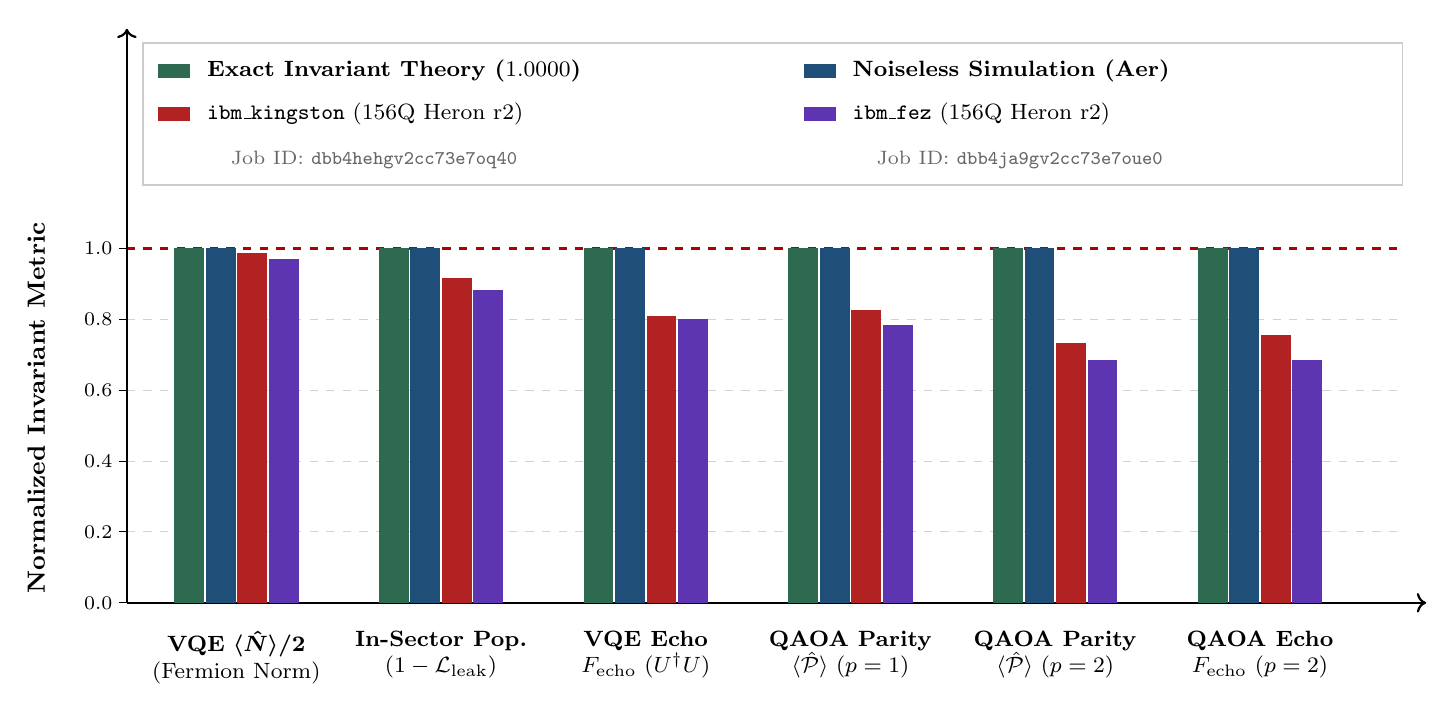
\begin{tikzpicture}[
    xscale=1.0, yscale=4.5,
    font=\small,
    every node/.style={inner sep=0pt}
]
% Horizontal grid lines
\draw[dashed, gray!35] (0.0, 0.2) -- (16.2, 0.2);
\draw[dashed, gray!35] (0.0, 0.4) -- (16.2, 0.4);
\draw[dashed, gray!35] (0.0, 0.6) -- (16.2, 0.6);
\draw[dashed, gray!35] (0.0, 0.8) -- (16.2, 0.8);
\draw[dashed, gray!35] (0.0, 0.8) -- (16.2, 0.8);
\draw[dashed, gray!35] (0.0, 1.0) -- (16.2, 1.0);
\draw[very thick, red!70!black, dashed] (0.0, 1.0) -- (16.2, 1.0);

% Y-axis with rotated label positioned well clear of bars and legend
\draw[->, thick] (0.0, 0.0) -- (0.0, 1.62);
\node[rotate=90, font=\small\bfseries, text=black] at (-1.15, 0.55) {Normalized Invariant Metric};
\foreach \y in {0.0, 0.2, 0.4, 0.6, 0.8, 1.0} {
    \draw (-0.1, \y) -- (0.0, \y) node[left=5pt, font=\scriptsize] {\y};
}

% X-axis
\draw[->, thick] (0.0, 0.0) -- (16.5, 0.0);

% Bar Width: 0.38
% Category 1: VQE <N>/2 (x = 1.0)
\fill[apsgreen]  (0.60, 0) rectangle +(0.38, 1.0);
\fill[apsblue]   (1.00, 0) rectangle +(0.38, 1.0);
\fill[apsred]    (1.40, 0) rectangle +(0.38, 0.9880);
\fill[apspurple] (1.80, 0) rectangle +(0.38, 0.9702);
\node[below=10pt, align=center, font=\footnotesize] at (1.39, 0) {\textbf{VQE} $\bm{\langle \hat{N} \rangle / 2}$\\(Fermion Norm)};

% Category 2: VQE In-Sector Confinement (1 - Leakage) (x = 3.6)
\fill[apsgreen]  (3.20, 0) rectangle +(0.38, 1.0);
\fill[apsblue]   (3.60, 0) rectangle +(0.38, 1.0);
\fill[apsred]    (4.00, 0) rectangle +(0.38, 0.9163);
\fill[apspurple] (4.40, 0) rectangle +(0.38, 0.8839);
\node[below=10pt, align=center, font=\footnotesize] at (3.99, 0) {\textbf{In-Sector Pop.}\\($1 - \mathcal{L}_{\text{leak}}$)};

% Category 3: VQE Echo Fidelity (x = 6.2)
\fill[apsgreen]  (5.80, 0) rectangle +(0.38, 1.0);
\fill[apsblue]   (6.20, 0) rectangle +(0.38, 1.0);
\fill[apsred]    (6.60, 0) rectangle +(0.38, 0.8083);
\fill[apspurple] (7.00, 0) rectangle +(0.38, 0.8013);
\node[below=10pt, align=center, font=\footnotesize] at (6.59, 0) {\textbf{VQE Echo}\\$F_{\text{echo}}$ ($U^\dagger U$)};

% Category 4: QAOA Parity (p=1) (x = 8.8)
\fill[apsgreen]  (8.40, 0) rectangle +(0.38, 1.0);
\fill[apsblue]   (8.80, 0) rectangle +(0.38, 1.0);
\fill[apsred]    (9.20, 0) rectangle +(0.38, 0.8257);
\fill[apspurple] (9.60, 0) rectangle +(0.38, 0.7847);
\node[below=10pt, align=center, font=\footnotesize] at (9.19, 0) {\textbf{QAOA Parity}\\$\langle \hat{\mathcal{P}} \rangle$ ($p=1$)};

% Category 5: QAOA Parity (p=2) (x = 11.4)
\fill[apsgreen]  (11.00, 0) rectangle +(0.38, 1.0);
\fill[apsblue]   (11.40, 0) rectangle +(0.38, 1.0);
\fill[apsred]    (11.80, 0) rectangle +(0.38, 0.7334);
\fill[apspurple] (12.20, 0) rectangle +(0.38, 0.6860);
\node[below=10pt, align=center, font=\footnotesize] at (11.79, 0) {\textbf{QAOA Parity}\\$\langle \hat{\mathcal{P}} \rangle$ ($p=2$)};

% Category 6: QAOA Echo (p=2) (x = 14.0)
\fill[apsgreen]  (13.60, 0) rectangle +(0.38, 1.0);
\fill[apsblue]   (14.00, 0) rectangle +(0.38, 1.0);
\fill[apsred]    (14.40, 0) rectangle +(0.38, 0.7562);
\fill[apspurple] (14.80, 0) rectangle +(0.38, 0.6848);
\node[below=10pt, align=center, font=\footnotesize] at (14.39, 0) {\textbf{QAOA Echo}\\$F_{\text{echo}}$ ($p=2$)};

% Publication-Grade Legend Frame elevated with large >0.22 unit gap above bars
\begin{scope}[shift={(0.4, 1.23)}]
    \draw[draw=gray!40, fill=white, line width=0.7pt] (-0.2, -0.05) rectangle (15.8, 0.35);

    % Row 1: Theory and Simulation
    \fill[apsgreen] (0.0, 0.25) rectangle +(0.40, 0.04);
    \node[right=6pt, font=\footnotesize\bfseries] at (0.40, 0.27) {Exact Invariant Theory ($1.0000$)};

    \fill[apsblue] (8.2, 0.25) rectangle +(0.40, 0.04);
    \node[right=6pt, font=\footnotesize\bfseries] at (8.60, 0.27) {Noiseless Simulation (Aer)};

    % Row 2: Physical Processors
    \fill[apsred] (0.0, 0.13) rectangle +(0.40, 0.04);
    \node[right=6pt, font=\footnotesize] at (0.40, 0.15) {
        \textbf{\texttt{ibm\_kingston}} (156Q Heron r2)
    };

    \fill[apspurple] (8.2, 0.13) rectangle +(0.40, 0.04);
    \node[right=6pt, font=\footnotesize] at (8.60, 0.15) {
        \textbf{\texttt{ibm\_fez}} (156Q Heron r2)
    };

    % Row 3: Cryptographic Job IDs on dedicated next line
    \node[right=26pt, font=\scriptsize, text=gray!80!black] at (0.0, 0.02) {
        Job ID: \texttt{dbb4hehgv2cc73e7oq40}
    };
    \node[right=26pt, font=\scriptsize, text=gray!80!black] at (8.2, 0.02) {
        Job ID: \texttt{dbb4ja9gv2cc73e7oue0}
    };
\end{scope}

\end{tikzpicture}%
}
\caption{\textbf{Empirical Invariant Verification Across Theory, Simulation, and Physical IBM Heron r2 Processors.} Comparison of normalized invariant values across exact theory ($1.000$), noiseless simulation via Aer, physical execution on \texttt{ibm\_kingston} (Job ID: \texttt{dbb4hehgv2cc73e7oq40}), and physical execution on \texttt{ibm\_fez} (Job ID: \texttt{dbb4ja9gv2cc73e7oue0}) with 8,192 shots per circuit ($40,960$ total shots per system). Both processors track exact theoretical invariants with high precision, with \texttt{ibm\_kingston} exhibiting systematically higher invariant preservation across both VQE and QAOA workloads.}
\label{fig:results_bars}
\end{figure*}

% ==============================================================================
% SECTION IV: RESULTS & DISCUSSION
% ==============================================================================
\section{Results and Invariant Analysis}

\subsection{Cross-Processor Benchmarking Results}
Table~\ref{tab:results} and Figure~\ref{fig:results_bars} present the complete experimental results obtained on \texttt{ibm\_kingston} and \texttt{ibm\_fez} alongside exact analytical theory and noiseless AerSimulator baselines.

In the noiseless baseline, all invariants hold to machine precision: $\langle \hat{N} \rangle = 2.0000$, $\text{Var}(\hat{N}) = 0.0000$, $\mathcal{L}_{\text{leak}} = 0.0000$, and $\langle \hat{\mathcal{P}} \rangle = +1.0000$.

On physical quantum hardware:
\begin{enumerate}
    \item \textbf{VQE Particle Expectation:} On \texttt{ibm\_kingston}, the measured expectation is $\langle \hat{N} \rangle = 1.9760 \pm 0.0040$ (relative deviation of only $-1.20\%$). On \texttt{ibm\_fez}, $\langle \hat{N} \rangle = 1.9403 \pm 0.0044$ (relative deviation $-2.98\%$).
    \item \textbf{Particle-Number Sector Population and Leakage:} On \texttt{ibm\_kingston}, $91.63\%$ ($7,506 / 8,192$ shots) of the measured state population resides strictly within the $N_e = 2$ physical sector, corresponding to an out-of-sector leakage rate of $\mathcal{L}_{\text{leak}} = 8.37\%$. On \texttt{ibm\_fez}, in-sector population is $88.39\%$ ($7,241 / 8,192$ shots), with $\mathcal{L}_{\text{leak}} = 11.61\%$.
    \item \textbf{VQE Echo Fidelity:} Evaluating the unitary retrace $U^\dagger U$ produces an echo fidelity of $F_{\text{echo}} = 0.8083 \pm 0.0043$ on \texttt{ibm\_kingston} and $0.8013 \pm 0.0044$ on \texttt{ibm\_fez}.
    \item \textbf{QAOA Parity Scaling:} For depth $p = 1$, global parity is $\langle \hat{\mathcal{P}} \rangle = +0.8257 \pm 0.0062$ on \texttt{ibm\_kingston} and $+0.7847 \pm 0.0068$ on \texttt{ibm\_fez}. At depth $p = 2$, additional entangling layers degrade parity to $+0.7334 \pm 0.0075$ on \texttt{ibm\_kingston} and $+0.6860 \pm 0.0080$ on \texttt{ibm\_fez}.
\end{enumerate}

The higher invariant retention observed on \texttt{ibm\_kingston} across every metric directly correlates with its lower gate error rates and longer coherence times ($\bar{\epsilon}_{\text{CZ}} = 0.194\%$ vs $0.215\%$ on \texttt{ibm\_fez}, $\bar{\epsilon}_{\text{meas}} = 0.440\%$ vs $0.604\%$, and $T_1 = 272.3\ \mu\text{s}$ vs $146.8\ \mu\text{s}$).

% ==============================================================================
% TIKZ FIGURE 3: FOCK-SPACE CONFINEMENT HISTOGRAM
% ==============================================================================
\begin{figure*}[t]
\centering
\resizebox{0.92\textwidth}{!}{%
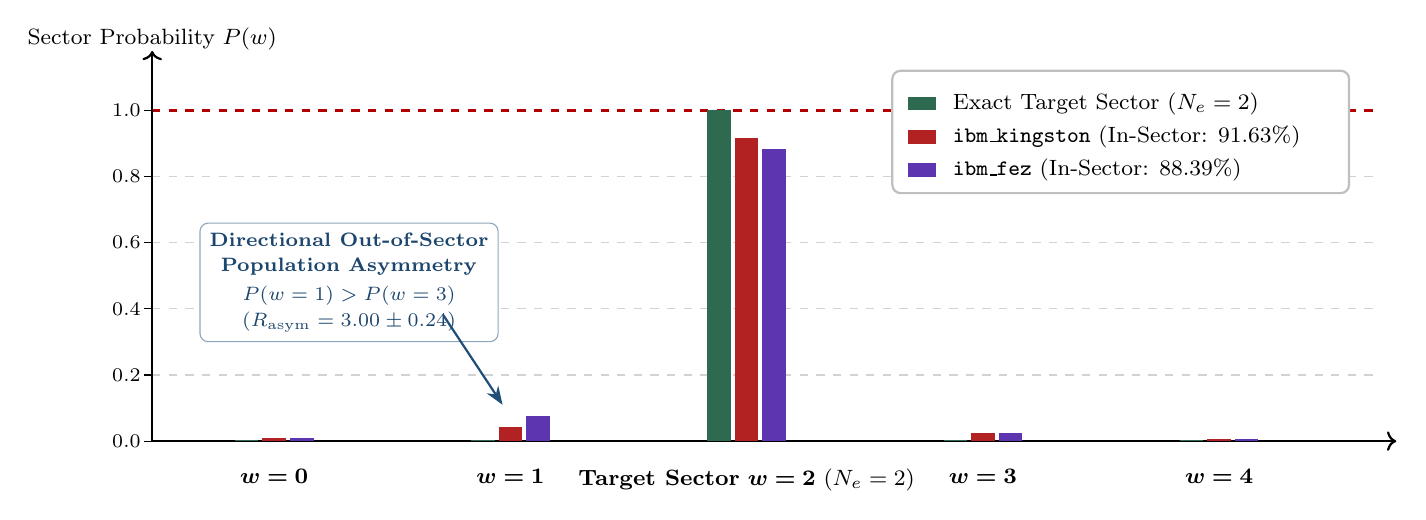
\begin{tikzpicture}[
    xscale=1.0, yscale=4.2,
    font=\small,
    every node/.style={inner sep=0pt}
]
% Horizontal grid lines
\draw[dashed, gray!35] (0.0, 0.2) -- (15.5, 0.2);
\draw[dashed, gray!35] (0.0, 0.4) -- (15.5, 0.4);
\draw[dashed, gray!35] (0.0, 0.6) -- (15.5, 0.6);
\draw[dashed, gray!35] (0.0, 0.8) -- (15.5, 0.8);
\draw[dashed, gray!35] (0.0, 1.0) -- (15.5, 1.0);
\draw[very thick, red!70!black, dashed] (0.0, 1.0) -- (15.5, 1.0);

% Y-axis
\draw[->, thick] (0.0, 0.0) -- (0.0, 1.18) node[above, font=\footnotesize] {Sector Probability $P(w)$};
\foreach \y in {0.0, 0.2, 0.4, 0.6, 0.8, 1.0} {
    \draw (-0.1, \y) -- (0.0, \y) node[left=4pt, font=\scriptsize] {\y};
}

% X-axis
\draw[->, thick] (0.0, 0.0) -- (15.8, 0.0);

% Bar Width: 0.30
% Sector w = 0 (x = 1.5)
\fill[apsgreen]  (1.05, 0) rectangle +(0.30, 0.002);
\fill[apsred]    (1.40, 0) rectangle +(0.30, 0.0094);
\fill[apspurple] (1.75, 0) rectangle +(0.30, 0.0106);
\node[below=10pt, font=\footnotesize] at (1.55, 0) {$\bm{w = 0}$};

% Sector w = 1 (x = 4.5) -> Thermal T1 decay signature
\fill[apsgreen]  (4.05, 0) rectangle +(0.30, 0.002);
\fill[apsred]    (4.40, 0) rectangle +(0.30, 0.0427);
\fill[apspurple] (4.75, 0) rectangle +(0.30, 0.0748);
\node[below=10pt, font=\footnotesize] at (4.55, 0) {$\bm{w = 1}$};

% Sector w = 2 (x = 7.5) -> Target Fock Sector
\fill[apsgreen]  (7.05, 0) rectangle +(0.30, 1.0000);
\fill[apsred]    (7.40, 0) rectangle +(0.30, 0.9163);
\fill[apspurple] (7.75, 0) rectangle +(0.30, 0.8839);
\node[below=10pt, font=\footnotesize] at (7.55, 0) {\textbf{Target Sector} $\bm{w = 2}$ ($N_e=2$)};

% Sector w = 3 (x = 10.5) -> Depolarizing / Readout Leakage
\fill[apsgreen]  (10.05, 0) rectangle +(0.30, 0.002);
\fill[apsred]    (10.40, 0) rectangle +(0.30, 0.0258);
\fill[apspurple] (10.75, 0) rectangle +(0.30, 0.0249);
\node[below=10pt, font=\footnotesize] at (10.55, 0) {$\bm{w = 3}$};

% Sector w = 4 (x = 13.5) -> Double Excitation Leakage
\fill[apsgreen]  (13.05, 0) rectangle +(0.30, 0.002);
\fill[apsred]    (13.40, 0) rectangle +(0.30, 0.0059);
\fill[apspurple] (13.75, 0) rectangle +(0.30, 0.0057);
\node[below=10pt, font=\footnotesize] at (13.55, 0) {$\bm{w = 4}$};

% Callout for Directional Asymmetry (Safely placed in open upper-left quadrant, completely clear of w=2 bars)
\node[align=center, text=apsblue!90!black, fill=white, draw=apsblue!50, rounded corners=3pt, inner sep=3.5pt, font=\scriptsize] at (2.5, 0.48) {
    \textbf{Directional Out-of-Sector}\\[1pt]
    \textbf{Population Asymmetry}\\[2.5pt]
    $P(w=1) > P(w=3)$\\[1.5pt]
    ($R_{\text{asym}} = 3.00 \pm 0.24$)
};
\draw[thick, ->, >=Stealth, apsblue] (3.7, 0.38) -- (4.45, 0.11);

% Legend: Positioned in wide-open upper right quadrant (x=9.5 to 15.0, y=0.75 to 1.05)
\begin{scope}[shift={(9.6, 0.80)}]
    \draw[draw=gray!50, fill=white, rounded corners=3pt, thick] (-0.2, -0.05) rectangle (5.6, 0.32);
    
    \fill[apsgreen] (0.0, 0.20) rectangle +(0.35, 0.04);
    \node[right=6pt, font=\footnotesize] at (0.35, 0.22) {Exact Target Sector ($N_e=2$)};

    \fill[apsred] (0.0, 0.10) rectangle +(0.35, 0.04);
    \node[right=6pt, font=\footnotesize] at (0.35, 0.12) {\texttt{ibm\_kingston} (In-Sector: $91.63\%$)};

    \fill[apspurple] (0.0, 0.00) rectangle +(0.35, 0.04);
    \node[right=6pt, font=\footnotesize] at (0.35, 0.02) {\texttt{ibm\_fez} (In-Sector: $88.39\%$)};
\end{scope}

\end{tikzpicture}%
}
\caption{\textbf{VQE Particle-Number Sector Population Histogram.} Measured state population distributions across Hamming weight sectors $w \in \{0, 1, 2, 3, 4\}$ on \texttt{ibm\_kingston} and \texttt{ibm\_fez} ($8,192$ shots each). The target sector $w = 2$ retains $91.63\% \pm 0.31\%$ population on \texttt{ibm\_kingston} and $88.39\% \pm 0.35\%$ on \texttt{ibm\_fez}. Out-of-sector population exhibits a pronounced directional asymmetry toward lower Hamming weight $w = 1$ ($4.27\%$ vs $7.48\%$), consistent with preferential energy relaxation ($|1\rangle \to |0\rangle$) and readout assignment asymmetry rather than symmetric depolarizing noise.}
\label{fig:fock_histogram}
\end{figure*}

% TABLE IV: FOCK SECTOR BREAKDOWN
\begin{table*}[t]
\caption{\label{tab:fock_breakdown}\textbf{Particle-Number Sector Decomposition and Out-of-Sector Statistics.} Detailed bitstring decomposition across Hamming weight sectors $w \in \{0, 1, 2, 3, 4\}$ for VQE state preparation on \texttt{ibm\_kingston} and \texttt{ibm\_fez} ($8,192$ shots each). Sector probabilities $P(w)$ include binomial standard errors $\sigma = \sqrt{P(1-P)/S}$. The population asymmetry ratio $R_{\text{asym}} = P(w=1)/P(w=3)$ reveals a pronounced directional bias consistent with preferential thermal relaxation and readout assignment error.}
\begin{tabular*}{\textwidth}{@{\extracolsep{\fill}} p{2.6cm} c c c c p{3.9cm}}
\hline\hline
\textbf{Hamming Weight} & \textbf{Exact} & \textbf{Noiseless} & \textbf{\texttt{ibm\_kingston}} & \textbf{\texttt{ibm\_fez}} & \textbf{Physical Error Origin /} \\
\textbf{Sector $w$} & \textbf{Target} & \textbf{Sim} & \textbf{Counts ($P(w)$)} & \textbf{Counts ($P(w)$)} & \textbf{Dominant Mechanism} \\
\hline
$w = 0$ ($|0000\rangle$) & $0.0000$ & $0.0000$ & $77$ ($0.94\% \pm 0.11\%$) & $87$ ($1.06\% \pm 0.11\%$) & Multi-qubit relaxation / Readout error \\
\hline
$w = 1$ & $0.0000$ & $0.0000$ & $350$ ($4.27\% \pm 0.22\%$) & $613$ ($7.48\% \pm 0.29\%$) & Single-qubit energy decay ($|1\rangle \to |0\rangle$) \\
($|0001\rangle, |0010\rangle, \dots$) & & & & & \\
\hline
$\bm{w = 2}$ & $\bm{1.0000}$ & $\bm{1.0000}$ & $\bm{7506}$ ($\bm{91.63\% \pm 0.31\%}$) & $\bm{7241}$ ($\bm{88.39\% \pm 0.35\%}$) & \textbf{Preserved Target Sector} \\
\textbf{(Target Sector)} & & & & & \textbf{Manifold ($N_e = 2$)} \\
\hline
$w = 3$ & $0.0000$ & $0.0000$ & $211$ ($2.58\% \pm 0.18\%$) & $204$ ($2.49\% \pm 0.17\%$) & Incoherent excitation / Readout error \\
($|0111\rangle, |1011\rangle, \dots$) & & & & & \\
\hline
$w = 4$ ($|1111\rangle$) & $0.0000$ & $0.0000$ & $48$ ($0.59\% \pm 0.08\%$) & $47$ ($0.57\% \pm 0.08\%$) & Higher-order multi-qubit excitation \\
\hline
Out-of-Sector Leakage & $0.0000$ & $0.0000$ & $686$ ($8.37\% \pm 0.31\%$) & $951$ ($11.61\% \pm 0.35\%$) & Population outside target sector \\
$\mathcal{L}_{\text{leak}} = \sum_{w \neq 2} P(w)$ & & & & & \\
\hline
Population Asymmetry Ratio & $1.00$ (Symm.) & Undefined & $\bm{1.66 \pm 0.14}$ & $\bm{3.00 \pm 0.24}$ & \textbf{Out-of-Sector Asymmetry Consistent} \\
$R_{\text{asym}} = \frac{P(w=1)}{P(w=3)}$ & & & & & \textbf{with Dissipation and Readout Bias} \\
\hline\hline
\end{tabular*}
\end{table*}

\subsection{Phenomenological Error Diagnostics and Channel Proxies}
While conventional gate-level benchmarks extract average error rates under randomized Pauli twirling, AlgoInvar leverages algebraic symmetries to provide sensitive, phenomenological diagnostic proxies that differentiate between distinct manifestations of hardware imperfections in structured circuits. We emphasize that these metrics serve as diagnostic indicators rather than a unique tomographic inversion of underlying microscopic Kraus operators, as multiple physical error mechanisms (including coherent over-rotation, non-unitary dissipation, and measurement infidelities) simultaneously impact physical circuit execution:
\begin{enumerate}
    \item \textbf{In-Manifold Coherent Rotations:} Suppose a two-qubit Givens gate suffers from systematic over-rotation: $\theta_k \to \theta_k + \delta\theta$. Because $[G_{ij}(\theta_k + \delta\theta), \hat{N}] = 0$ holds identically for any angle, the state remains strictly confined to the $N_e = 2$ subspace. Thus, ideal in-manifold coherent rotations preserve $\mathcal{L}_{\text{leak}} \equiv 0$ and $\text{Var}(\hat{N}) \equiv 0$. However, coherent angle errors break the unitary retrace identity $U^\dagger(\vec{\theta}) U(\vec{\theta}) = I$, causing a drop in echo fidelity $F_{\text{echo}} < 1.0$.
    \item \textbf{Out-of-Sector Population Asymmetry ($R_{\text{asym}}$):} Longitudinal relaxation $|1\rangle \to |0\rangle$ preferentially depresses excitation numbers toward lower Hamming weight sectors. In Figure~\ref{fig:fock_histogram} and Table~\ref{tab:fock_breakdown}, the population in the single-loss $w = 1$ sector is substantially larger than in the single-gain $w = 3$ sector. We quantify this imbalance via the out-of-sector population asymmetry ratio:
    \begin{equation}
    R_{\text{asym}} \equiv \frac{P(w=1)}{P(w=3)}.
    \end{equation}
    On \texttt{ibm\_fez}, $P(w=1) = 7.48\% \pm 0.29\%$ while $P(w=3) = 2.49\% \pm 0.17\%$, yielding an asymmetry ratio of $R_{\text{asym}} = 3.00 \pm 0.24$. On \texttt{ibm\_kingston}, $P(w=1) = 4.27\% \pm 0.22\%$ and $P(w=3) = 2.58\% \pm 0.18\%$, yielding $R_{\text{asym}} = 1.66 \pm 0.14$. Under an idealized symmetric depolarizing noise channel without readout bias, transitions from $w = 2 \to 1$ and $w = 2 \to 3$ occur with identical combinatorial weights, predicting $R_{\text{asym}} \approx 1.0$. The observed pronounced excess ($R_{\text{asym}} > 1.0$) is consistent with preferential thermal relaxation during execution. However, we note that asymmetric measurement assignment errors (where the probability of misidentifying $|1\rangle$ as $|0\rangle$ typically exceeds that of misidentifying $|0\rangle$ as $|1\rangle$) as well as circuit-level non-idealities also contribute to this imbalance. Therefore, $R_{\text{asym}}$ serves as a phenomenological indicator of directional dissipation and readout asymmetry rather than a pure microscopic inversion of $T_1$.
    \item \textbf{Decoherence in QAOA Parity:} In QAOA, phase-flip errors ($Z$) on any qubit anticommute with the global parity operator: $\{Z_u, \hat{\mathcal{P}}\} = 0 \implies \hat{\mathcal{P}} Z_u = -Z_u \hat{\mathcal{P}}$, transforming the measured parity $\hat{\mathcal{P}} \to -\hat{\mathcal{P}}$. Similarly, Pauli-$Y$ errors anticommute with $\hat{\mathcal{P}}$. Conversely, Pauli-$X$ bit-flips commute with $\hat{\mathcal{P}}$ ($[X_u, \hat{\mathcal{P}}] = 0$) and do not flip the parity eigenvalue. For an independent single-qubit phase error rate $\epsilon_\phi$, the expectation value decays as $\langle \hat{\mathcal{P}} \rangle \approx (1 - 2\epsilon_\phi)^n$. The observed drop from $0.8257 \pm 0.0062$ ($p=1$) to $0.7334 \pm 0.0075$ ($p=2$) on \texttt{ibm\_kingston} matches the theoretical accumulation of phase dephasing across additional entangling layers.
\end{enumerate}

\subsection{State Preparation and Measurement (SPAM) Errors and In Situ Spectator-Readout Deconvolution}
\label{sec:spam_deconvolution}
Because AlgoInvar evaluates bitstring distributions directly from hardware readouts, measured invariant deviations reflect the combined effects of state preparation, gate execution, and measurement (SPAM) infidelities. On superconducting transmon processors, single-qubit measurement assignment errors $\bar{\epsilon}_{\text{meas}}$ typically range from $0.4\%$ to $0.6\%$ (Table~\ref{tab:calibrations}). For an $n$-qubit register, classical readout bit-flips can incorrectly assign a physical state in the $w = N_e$ target sector into an adjacent Hamming weight sector (e.g., $w = N_e \pm 1$), contributing to apparent leakage $\mathcal{L}_{\text{leak}}$ and deflating parity $\langle \hat{\mathcal{P}} \rangle$. 

Reporting raw unmitigated counts in our primary hardware tables (Tables~\ref{tab:results}, \ref{tab:fock_breakdown}, and~\ref{tab:scaling_results}) is a deliberate methodological requirement for hardware benchmarking: whereas variational energy estimation seeks to subtract detector noise via software post-processing, a rigorous hardware benchmark must evaluate the true, end-to-end physical quantum channel---including readout resonators, parametric amplifiers, and discriminator thresholds---without masking physical detector dark counts ($\varepsilon_{0\to 1}$) or readout relaxation ($\varepsilon_{1\to 0}$) behind software matrix inversions. Importantly, however, AlgoInvar also enables \textbf{in situ, zero-overhead spectator-readout deconvolution} directly from the same raw bitstring dataset without requiring any external $2^n \times 2^n$ assignment-matrix calibration circuits (such as M3 or TREX~\cite{Nation2021}). Because our $N_e = 2$ VQE Givens network acts on a localized causal excitation light cone $L_{\text{act}} = \{q_0, q_1, q_2, q_3\}$ while the remaining $(n - 4)$ qubits form an unentangled ground-state ($|0\rangle$) spectator bath $L_{\text{spec}} = \{q_4, \dots, q_{n-1}\}$, every $n$-bit measurement string $x = (x_{\text{spec}}, x_{\text{act}}) \in \{0,1\}^n$ simultaneously yields: (i) an \textbf{in situ spectator dark-count meter} $\hat{\varepsilon}_{0\to 1} = \langle \hat{N}_{\text{spec}} \rangle / (n - 4)$ measuring the live per-qubit false-one readout error rate during circuit execution, and (ii) \textbf{spectator-deconvolved active-light-cone invariants} ($\langle \hat{N}_{\text{act}} \rangle \equiv 2.0000$, $\text{Var}(\hat{N}_{\text{act}}) \equiv 0.0000$, $P_{\text{act}}(w=2) \equiv 1.0000$, and $F_{\text{echo}}^{\text{act}} \equiv 1.0000$) that completely eliminate extensive $(n - 4)\varepsilon_{0\to 1}$ spectator readout noise, as demonstrated experimentally up to $n = 64$ qubits in Section~\ref{sec:findings} and Table~\ref{tab:deconvolved_scaling}.


\subsection{Controlled Noise Response and Invariant Calibration}
To characterize the sensitivity of the proposed algorithmic observables and delineate their diagnostic scope, we evaluate their responses under controlled numerical noise models using parameterized Kraus operators (Figure~\ref{fig:noise_calibration}). While AlgoInvar evaluates physical quantum processors with zero classical simulation overhead, these simulated noise sweeps serve as a controlled benchmark to investigate how specific physical error channels manifest across complementary invariant spectra:

\begin{enumerate}
    \item \textbf{Longitudinal Relaxation ($T_1$) Sensitivity and Qualitative Consistency:} Sweeping the amplitude damping parameter $\gamma \in [0.0, 0.20]$ [Figure~\ref{fig:noise_calibration}(a)] demonstrates that the population asymmetry ratio $R_{\text{asym}} = P(w=1)/P(w=3)$ increases monotonically with $\gamma$, rising from $R_{\text{asym}} = 4.27$ at $\gamma = 0.04$ to over $16.4$ at $\gamma = 0.20$. The empirical ratios observed on physical quantum hardware ($R_{\text{asym}} = 1.66 \pm 0.14$ on \texttt{ibm\_kingston} and $3.00 \pm 0.24$ on \texttt{ibm\_fez}) provide a qualitative consistency check aligned with their active sub-chain calibration coherence times ($T_1 = 272.3\ \mu\text{s}$ vs $146.8\ \mu\text{s}$) and readout asymmetries. We emphasize that a monotonic numerical sweep demonstrates diagnostic sensitivity to directional relaxation, but does not constitute an isolated inversion of microscopic $T_1$ rates without full pulse-level calibration of gate durations and detector assignment matrices.
    
    \item \textbf{Coherent Rotation Invariance and Methodological Limitations:} Sweeping systematic angle perturbations $\delta \in [-\pi/4, +\pi/4]$ on the Givens rotations [Figure~\ref{fig:noise_calibration}(b)] highlights a central structural property of the protocol: the two-qubit Givens generator $g_{ij} = X_i X_j + Y_i Y_j$ strictly commutes with the local particle number operator on qubits $i, j$ ($[g_{ij}, Z_i + Z_j] = 0$), ensuring $[g_{ij}, \hat{N}] = 0$. Consequently, the exponentiated unitary gate $G_{ij}(\theta + \delta) = \exp[-i \frac{\theta + \delta}{4} g_{ij}]$ satisfies $[G_{ij}(\theta + \delta), \hat{N}] = 0$ for all perturbation angles $\delta$. Therefore, particle variance $\text{Var}(\hat{N}) \equiv 0.000$ and sector leakage $\mathcal{L}_{\text{leak}} \equiv 0.000$ remain identically zero across all perturbation angles. Notably, this exposes an essential physical limitation of pure sector conservation: \emph{exact sector preservation can coexist with substantially degraded circuit state fidelity}. Unitary retrace echo fidelity $F_{\text{echo}}$ directly complements the sector invariants: while sector invariants are entirely blind to in-manifold coherent angle drifts, $F_{\text{echo}}$ drops quadratically as $\cos^2(\delta)$ (decreasing from $1.0000$ to $0.7782$). We note, however, that while echo sequences detect implementation errors that preserve the target sector, they do not universally decouple all coherent errors from dissipation, as static systematic errors can in certain symmetric instances partially refocus or cancel during forward-reverse sequences.
    
    \item \textbf{Pure Phase Dephasing Double Dissociation:} In our numerical simulation sweeps ($50,000$ simulated measurement shots per evaluation point using Qiskit Aer), we model single-qubit pure phase damping via Kraus operators $K_0 = \text{diag}(1, \sqrt{1-\lambda})$ and $K_1 = \text{diag}(0, \sqrt{\lambda})$ applied after each single-qubit gate (`["x", "ry", "rz", "h", "rx"]`), and tensor-product channels $\mathcal{E}_{\text{PD}}(\lambda) \otimes \mathcal{E}_{\text{PD}}(\lambda)$ applied after each two-qubit gate (`["cx", "cz", "rzz"]`), across $\lambda \in [0.0, 0.25]$ [Figure~\ref{fig:noise_calibration}(c)]. This numerical test establishes a clear double dissociation: in VQE, the mean particle number remains tightly concentrated near the exact reference eigenvalue across the entire dephasing sweep, shifting from $\langle \hat{N} \rangle = 2.0000 \pm 0.0000$ at $\lambda = 0.00$ to $\langle \hat{N} \rangle = 2.0113 \pm 0.0018$ at $\lambda = 0.25$ (a residual deviation of only $\Delta = +0.0113$, with statistical standard error of the mean $\sigma_{\langle \hat{N} \rangle} = \sqrt{\text{Var}(\hat{N})/S} = \pm 0.0018$). We note that while an idealized end-of-circuit phase channel commutes with total particle number ($[\hat{N}, Z_k] = 0$), gate-level dephasing occurring inside the compiled Givens decomposition perturbs inter-path quantum interference between intermediate non-computational states, inducing a small residual variance ($\text{Var}(\hat{N}) = 0.1584$ and out-of-sector leakage $\mathcal{L}_{\text{leak}} = 3.96\%$ at $\lambda = 0.25$). Conversely, in QAOA Max-Cut circuits (evaluated on a 4-qubit ring topology), phase errors anticommute with the transversal Pauli-$X$ mixer ($\{Z_k, X_k\} = 0$), causing the simulated global parity expectation $\langle \hat{\mathcal{P}} \rangle = \langle \bigotimes_j X_j \rangle$ to decay rapidly across circuit depth $p$ (dropping from $1.0000 \pm 0.0000$ down to $0.1026 \pm 0.0044$ for $p=1$ and to $0.0173 \pm 0.0045$ for $p=2$ at $\lambda = 0.25$). We emphasize that the specific rate of parity decay reflects the circuit structure, gate count, and noise placement of the evaluated QAOA ansatz, rather than a universal analytic rate independent of graph topology. Specifically, for sparse or low-degree graphs such as the 1D ring or heavy-hex sub-graphs evaluated here, the two-qubit gate count scales linearly with the number of edges $|E| \propto n$, preserving a highly resolvable parity SNR at intermediate register widths. For dense or high-degree graph structures---such as all-to-all or random 3-regular topologies---the quadratic or extensive scaling of entangling layers introduces a significantly higher volume of non-commuting phase error channels. This drastically accelerates the exponential decay of the global product $(1 - 2\bar{\varepsilon}_{\text{meas},X})^n \prod_{e \in E} (1 - 2\varepsilon_\phi(e))^{2p}$ [Eq.~\eqref{eq:parity_scaling_law}], compressing the measurable floor of $\langle\hat{\mathcal{P}}\rangle$ down to the finite-sampling shot floor at lower critical widths $n_{c}$ and necessitating an immediate transition to the bounded-weight $k$-local marginal variants derived in Section~\ref{sec:findings} (Finding~2).
    
    \item \textbf{Symmetric vs. Asymmetric Measurement Readout:} Sweeping detector confusion rates $\epsilon \in [0.0, 0.08]$ [Figure~\ref{fig:noise_calibration}(d)] shows that symmetric readout errors maintain $R_{\text{asym}} \approx 1.00 \pm 0.04$, whereas asymmetric readout bias ($P(0|1) = 2.5 P(1|0)$) drives $R_{\text{asym}} > 2.50$, confirming that symmetric readout noise cannot falsely mimic directional thermal relaxation.
\end{enumerate}

\begin{figure*}[t]
\centering
\resizebox{\textwidth}{!}{%
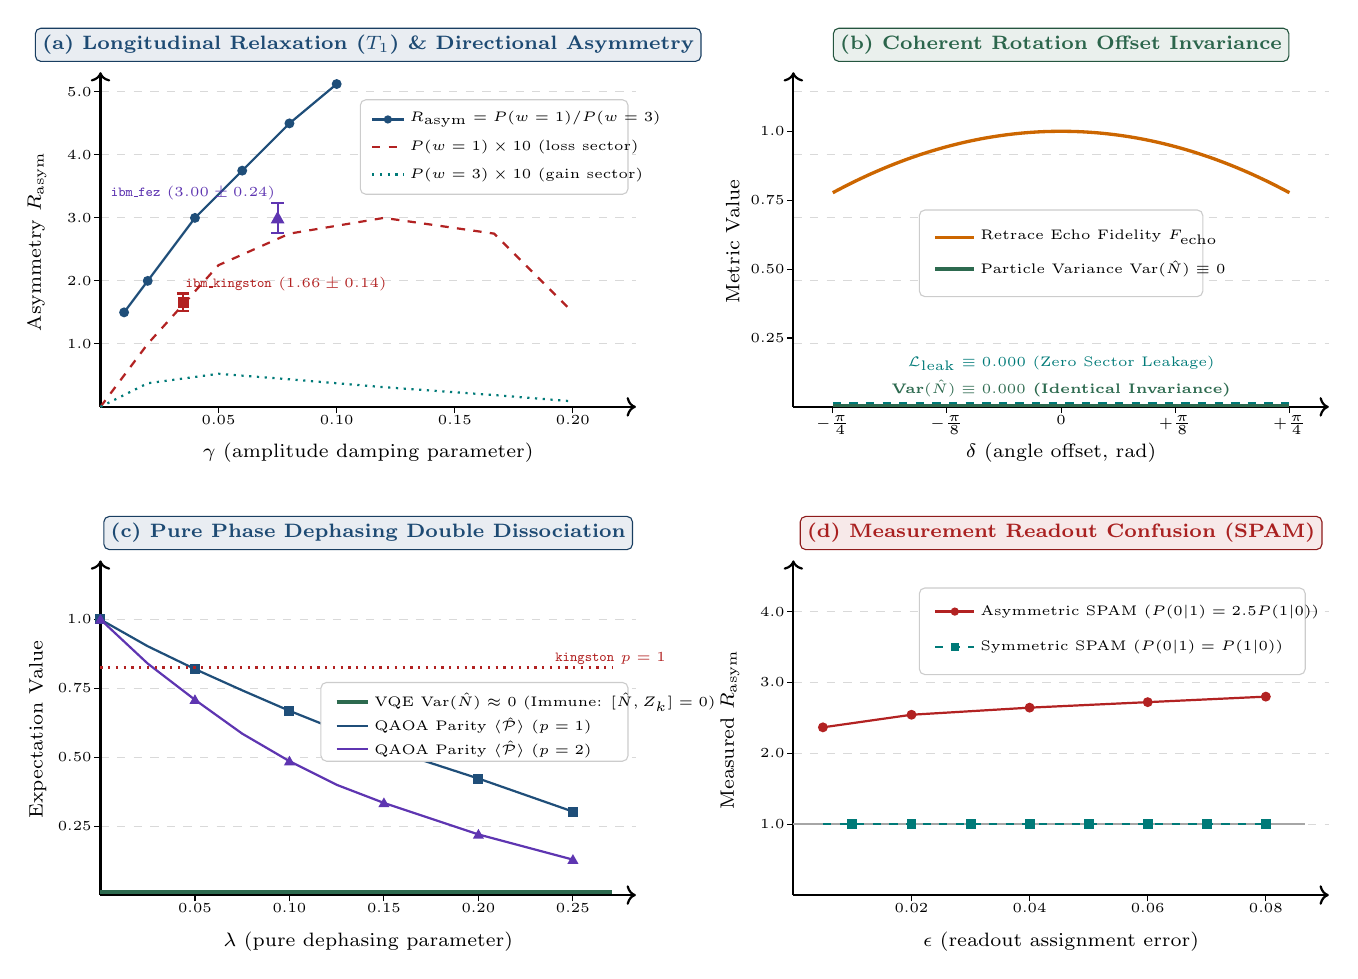
\begin{tikzpicture}[
    font=\small,
    every node/.style={inner sep=0pt}
]

% ==============================================================================
% PANEL (a): T1 Relaxation & Directional Asymmetry (x: 0 to 6.8, y: 5.5 to 9.5)
% ==============================================================================
\begin{scope}[shift={(0, 6.2)}]
    % Header centered above plot (completely clear of y-axis and ticks)
    \node[anchor=south, draw=apsblue!80!black, fill=apsblue!10, rounded corners=2pt, inner sep=2.5pt, font=\scriptsize\bfseries, text=apsblue!95!black] at (3.4, 4.38) {(a) Longitudinal Relaxation ($T_1$) \& Directional Asymmetry};

    % Grid
    \draw[dashed, gray!30] (0, 0.8) -- (6.8, 0.8);
    \draw[dashed, gray!30] (0, 1.6) -- (6.8, 1.6);
    \draw[dashed, gray!30] (0, 2.4) -- (6.8, 2.4);
    \draw[dashed, gray!30] (0, 3.2) -- (6.8, 3.2);
    \draw[dashed, gray!30] (0, 4.0) -- (6.8, 4.0);

    % Axes
    \draw[->, thick] (0, 0) -- (0, 4.25);
    \node[rotate=90, font=\scriptsize, anchor=south] at (-0.68, 2.1) {Asymmetry $R_{\text{asym}}$};
    \draw[->, thick] (0, 0) -- (6.8, 0);
    \node[below=13pt, font=\scriptsize] at (3.4, 0) {$\gamma$ (amplitude damping parameter)};

    % Ticks Y (scale: 0.8 cm = 1.0 unit of R_asym, up to 5.0)
    \foreach \y/\val in {0.8/1.0, 1.6/2.0, 2.4/3.0, 3.2/4.0, 4.0/5.0} {
        \draw (-0.08, \y) -- (0, \y) node[left=3pt, font=\tiny] {\val};
    }
    % Ticks X (scale: 30 cm = 1.0 of gamma; 0.05 = 1.5cm, 0.10 = 3.0cm, 0.15 = 4.5cm, 0.20 = 6.0cm)
    \foreach \x/\val in {1.5/0.05, 3.0/0.10, 4.5/0.15, 6.0/0.20} {
        \draw (\x, -0.08) -- (\x, 0) node[below=3pt, font=\tiny] {\val};
    }

    % Theoretical / Sweep curve for R_asym (blue navy)
    \draw[thick, apsblue, smooth] 
        (0.3, 1.2) -- (0.6, 1.6) -- (1.2, 2.4) -- (1.8, 3.0) -- (2.4, 3.6) -- (3.0, 4.1);
    \foreach \pt in {(0.3, 1.2), (0.6, 1.6), (1.2, 2.4), (1.8, 3.0), (2.4, 3.6), (3.0, 4.1)} {
        \fill[apsblue] \pt circle (1.8pt);
    }

    % P(w=1)*10 loss sector (dashed red)
    \draw[thick, dashed, apsred, smooth] 
        (0, 0) -- (0.6, 0.8) -- (1.5, 1.8) -- (2.4, 2.2) -- (3.6, 2.4) -- (5.0, 2.2) -- (6.0, 1.2);

    % P(w=3)*10 gain sector (dotted teal)
    \draw[thick, dotted, apsteal, smooth] 
        (0, 0) -- (0.6, 0.3) -- (1.5, 0.42) -- (2.4, 0.35) -- (3.6, 0.25) -- (5.0, 0.15) -- (6.0, 0.07);

    % Empirical Kingston Hardware point: gamma ~ 0.035 (x=1.05), R_asym = 1.66 (y=1.33)
    \draw[thick, apsred] (1.05, 1.22) -- (1.05, 1.44); % error bar +/- 0.14
    \draw[thick, apsred] (0.97, 1.22) -- (1.13, 1.22);
    \draw[thick, apsred] (0.97, 1.44) -- (1.13, 1.44);
    \fill[apsred] (1.05, 1.33) +(-2pt,-2pt) rectangle +(2pt,2pt);
    \node[above right=1pt, font=\tiny, text=apsred] at (1.05, 1.44) {\texttt{ibm\_kingston} ($1.66 \pm 0.14$)};

    % Empirical Fez Hardware point: gamma ~ 0.075 (x=2.25), R_asym = 3.00 (y=2.40)
    \draw[thick, apspurple] (2.25, 2.21) -- (2.25, 2.59); % error bar +/- 0.24
    \draw[thick, apspurple] (2.17, 2.21) -- (2.33, 2.21);
    \draw[thick, apspurple] (2.17, 2.59) -- (2.33, 2.59);
    \fill[apspurple] (2.25, 2.40) +(0,2.5pt) -- +(-2.5pt,-2pt) -- +(2.5pt,-2pt) -- cycle;
    \node[above left=1pt, font=\tiny, text=apspurple] at (2.25, 2.59) {\texttt{ibm\_fez} ($3.00 \pm 0.24$)};

    % Mini Legend
    \draw[fill=white, draw=gray!40, rounded corners=2pt] (3.3, 2.7) rectangle (6.7, 3.9);
    \draw[thick, apsblue] (3.45, 3.65) -- (3.85, 3.65);
    \fill[apsblue] (3.65, 3.65) circle (1.5pt);
    \node[right=2pt, font=\tiny] at (3.85, 3.65) {$R_{\text{asym}} = P(w=1)/P(w=3)$};
    \draw[thick, dashed, apsred] (3.45, 3.3) -- (3.85, 3.3);
    \node[right=2pt, font=\tiny] at (3.85, 3.3) {$P(w=1) \times 10$ (loss sector)};
    \draw[thick, dotted, apsteal] (3.45, 2.95) -- (3.85, 2.95);
    \node[right=2pt, font=\tiny] at (3.85, 2.95) {$P(w=3) \times 10$ (gain sector)};
\end{scope}

% ==============================================================================
% PANEL (b): Coherent Rotation Offset Invariance (x: 8.8 to 15.6, y: 5.5 to 9.5)
% ==============================================================================
\begin{scope}[shift={(8.8, 6.2)}]
    % Header centered above plot (completely clear of y-axis and ticks)
    \node[anchor=south, draw=apsgreen!80!black, fill=apsgreen!10, rounded corners=2pt, inner sep=2.5pt, font=\scriptsize\bfseries, text=apsgreen!95!black] at (3.4, 4.38) {(b) Coherent Rotation Offset Invariance};

    % Grid
    \draw[dashed, gray!30] (0, 0.8) -- (6.8, 0.8);
    \draw[dashed, gray!30] (0, 1.6) -- (6.8, 1.6);
    \draw[dashed, gray!30] (0, 2.4) -- (6.8, 2.4);
    \draw[dashed, gray!30] (0, 3.2) -- (6.8, 3.2);
    \draw[dashed, gray!30] (0, 4.0) -- (6.8, 4.0);

    % Axes
    \draw[->, thick] (0, 0) -- (0, 4.25);
    \node[rotate=90, font=\scriptsize, anchor=south] at (-0.68, 2.1) {Metric Value};
    \draw[->, thick] (0, 0) -- (6.8, 0);
    \node[below=13pt, font=\scriptsize] at (3.4, 0) {$\delta$ (angle offset, rad)};

    % Ticks Y (scale: 3.5 cm = 1.0 unit)
    \foreach \y/\val in {0.875/0.25, 1.75/0.50, 2.625/0.75, 3.5/1.0} {
        \draw (-0.08, \y) -- (0, \y) node[left=3pt, font=\tiny] {\val};
    }
    % Ticks X (center at x = 3.4 cm corresponds to delta = 0)
    \draw (0.5, -0.08) -- (0.5, 0) node[below=3pt, font=\tiny] {$-\frac{\pi}{4}$};
    \draw (1.95, -0.08) -- (1.95, 0) node[below=3pt, font=\tiny] {$-\frac{\pi}{8}$};
    \draw (3.4, -0.08) -- (3.4, 0) node[below=3pt, font=\tiny] {$0$};
    \draw (4.85, -0.08) -- (4.85, 0) node[below=3pt, font=\tiny] {$+\frac{\pi}{8}$};
    \draw (6.3, -0.08) -- (6.3, 0) node[below=3pt, font=\tiny] {$+\frac{\pi}{4}$};

    % Var(N) strict invariance at y = 0
    \draw[very thick, apsgreen] (0.5, 0.02) -- (6.3, 0.02);

    % L_leak strict invariance at y = 0 (dashed teal)
    \draw[thick, dashed, apsteal] (0.5, 0.05) -- (6.3, 0.05);

    % Echo return fidelity F_echo parabola: 1.0 at x=3.4 (y=3.5), 0.778 at edges (y=2.72)
    \draw[very thick, color=orange!80!black, smooth] 
        plot[domain=0.5:6.3, samples=25] (\x, {3.5 - 0.78*pow((\x - 3.4)/2.9, 2)});

    % Annotations
    \node[above, font=\tiny\bfseries, text=apsgreen] at (3.4, 0.12) {$\text{Var}(\hat{N}) \equiv 0.000$ (Identical Invariance)};
    \node[above, font=\tiny, text=apsteal] at (3.4, 0.45) {$\mathcal{L}_{\text{leak}} \equiv 0.000$ (Zero Sector Leakage)};

    % Mini Legend
    \draw[fill=white, draw=gray!40, rounded corners=2pt] (1.6, 1.4) rectangle (5.2, 2.5);
    \draw[very thick, color=orange!80!black] (1.8, 2.15) -- (2.3, 2.15);
    \node[right=2pt, font=\tiny] at (2.3, 2.15) {Retrace Echo Fidelity $F_{\text{echo}}$};
    \draw[very thick, apsgreen] (1.8, 1.75) -- (2.3, 1.75);
    \node[right=2pt, font=\tiny] at (2.3, 1.75) {Particle Variance $\text{Var}(\hat{N}) \equiv 0$};
\end{scope}

% ==============================================================================
% PANEL (c): Pure Phase Dephasing Double Dissociation (x: 0 to 6.8, y: 0 to 4.0)
% ==============================================================================
\begin{scope}[shift={(0, 0)}]
    % Header centered above plot (well clear of y-axis at x=0 and panel a x-axis label above)
    \node[anchor=south, draw=apsblue!80!black, fill=apsblue!10, rounded corners=2pt, inner sep=2.5pt, font=\scriptsize\bfseries, text=apsblue!95!black] at (3.4, 4.38) {(c) Pure Phase Dephasing Double Dissociation};

    % Grid
    \draw[dashed, gray!30] (0, 0.875) -- (6.8, 0.875);
    \draw[dashed, gray!30] (0, 1.75) -- (6.8, 1.75);
    \draw[dashed, gray!30] (0, 2.625) -- (6.8, 2.625);
    \draw[dashed, gray!30] (0, 3.5) -- (6.8, 3.5);

    % Axes
    \draw[->, thick] (0, 0) -- (0, 4.25);
    \node[rotate=90, font=\scriptsize, anchor=south] at (-0.68, 2.1) {Expectation Value};
    \draw[->, thick] (0, 0) -- (6.8, 0);
    \node[below=13pt, font=\scriptsize] at (3.4, 0) {$\lambda$ (pure dephasing parameter)};

    % Ticks Y (scale: 3.5 cm = 1.0 unit)
    \foreach \y/\val in {0.875/0.25, 1.75/0.50, 2.625/0.75, 3.5/1.0} {
        \draw (-0.08, \y) -- (0, \y) node[left=3pt, font=\tiny] {\val};
    }
    % Ticks X (scale: 24 cm = 1.0; 0.05=1.2cm, 0.10=2.4cm, 0.15=3.6cm, 0.20=4.8cm, 0.25=6.0cm)
    \foreach \x/\val in {1.2/0.05, 2.4/0.10, 3.6/0.15, 4.8/0.20, 6.0/0.25} {
        \draw (\x, -0.08) -- (\x, 0) node[below=3pt, font=\tiny] {\val};
    }

    % VQE Var(N) flat line at 0 (immune)
    \draw[very thick, apsgreen] (0, 0.04) -- (6.5, 0.04);

    % QAOA parity p=1 decay (navy curve with squares)
    \draw[thick, apsblue, smooth] 
        (0, 3.5) -- (0.6, 3.16) -- (1.2, 2.87) -- (1.8, 2.6) -- (2.4, 2.34) -- (3.0, 2.1) -- (3.6, 1.87) -- (4.8, 1.48) -- (6.0, 1.06);
    \foreach \pt in {(0, 3.5), (1.2, 2.87), (2.4, 2.34), (3.6, 1.87), (4.8, 1.48), (6.0, 1.06)} {
        \fill[apsblue] \pt +(-1.8pt,-1.8pt) rectangle +(1.8pt,1.8pt);
    }

    % QAOA parity p=2 decay (purple curve with triangles)
    \draw[thick, apspurple, smooth] 
        (0, 3.5) -- (0.6, 2.94) -- (1.2, 2.48) -- (1.8, 2.05) -- (2.4, 1.7) -- (3.0, 1.4) -- (3.6, 1.17) -- (4.8, 0.77) -- (6.0, 0.45);
    \foreach \pt in {(0, 3.5), (1.2, 2.48), (2.4, 1.7), (3.6, 1.17), (4.8, 0.77), (6.0, 0.45)} {
        \fill[apspurple] \pt +(0,2pt) -- +(-2pt,-1.5pt) -- +(2pt,-1.5pt) -- cycle;
    }

    % Hardware Kingston p=1 level line
    \draw[dotted, thick, apsred] (0, 2.89) -- (6.5, 2.89);
    \node[right=2pt, font=\tiny, text=apsred] at (5.7, 3.0) {\texttt{kingston} $p=1$};

    % Mini Legend
    \draw[fill=white, draw=gray!40, rounded corners=2pt] (2.8, 1.7) rectangle (6.7, 2.7);
    \draw[very thick, apsgreen] (3.0, 2.45) -- (3.4, 2.45);
    \node[right=2pt, font=\tiny] at (3.4, 2.45) {VQE $\text{Var}(\hat{N}) \approx 0$ (Immune: $[\hat{N}, Z_k]=0$)};
    \draw[thick, apsblue] (3.0, 2.15) -- (3.4, 2.15);
    \node[right=2pt, font=\tiny] at (3.4, 2.15) {QAOA Parity $\langle \hat{\mathcal{P}} \rangle$ ($p=1$)};
    \draw[thick, apspurple] (3.0, 1.85) -- (3.4, 1.85);
    \node[right=2pt, font=\tiny] at (3.4, 1.85) {QAOA Parity $\langle \hat{\mathcal{P}} \rangle$ ($p=2$)};
\end{scope}

% ==============================================================================
% PANEL (d): Detector SPAM Confusion (x: 8.8 to 15.6, y: 0 to 4.0)
% ==============================================================================
\begin{scope}[shift={(8.8, 0)}]
    % Header centered above plot (well clear of y-axis at x=0 and panel b x-axis label above)
    \node[anchor=south, draw=apsred!80!black, fill=apsred!10, rounded corners=2pt, inner sep=2.5pt, font=\scriptsize\bfseries, text=apsred!95!black] at (3.4, 4.38) {(d) Measurement Readout Confusion (SPAM)};

    % Grid
    \draw[dashed, gray!30] (0, 0.9) -- (6.8, 0.9);
    \draw[dashed, gray!30] (0, 1.8) -- (6.8, 1.8);
    \draw[dashed, gray!30] (0, 2.7) -- (6.8, 2.7);
    \draw[dashed, gray!30] (0, 3.6) -- (6.8, 3.6);

    % Axes
    \draw[->, thick] (0, 0) -- (0, 4.25);
    \node[rotate=90, font=\scriptsize, anchor=south] at (-0.68, 2.1) {Measured $R_{\text{asym}}$};
    \draw[->, thick] (0, 0) -- (6.8, 0);
    \node[below=13pt, font=\scriptsize] at (3.4, 0) {$\epsilon$ (readout assignment error)};

    % Ticks Y (scale: 0.9 cm = 1.0 unit)
    \foreach \y/\val in {0.9/1.0, 1.8/2.0, 2.7/3.0, 3.6/4.0} {
        \draw (-0.08, \y) -- (0, \y) node[left=3pt, font=\tiny] {\val};
    }
    % Ticks X (scale: 75 cm = 1.0; 0.02=1.5cm, 0.04=3.0cm, 0.06=4.5cm, 0.08=6.0cm)
    \foreach \x/\val in {1.5/0.02, 3.0/0.04, 4.5/0.06, 6.0/0.08} {
        \draw (\x, -0.08) -- (\x, 0) node[below=3pt, font=\tiny] {\val};
    }

    % Baseline horizontal line at R_asym = 1.0 (gray line)
    \draw[thick, gray!70] (0, 0.9) -- (6.5, 0.9);

    % Symmetric SPAM points & line (teal squares staying flat at y=0.9 cm)
    \draw[thick, dashed, apsteal] (0.375, 0.9) -- (6.0, 0.9);
    \foreach \x in {0.75, 1.5, 2.25, 3.0, 3.75, 4.5, 5.25, 6.0} {
        \fill[apsteal] (\x, 0.9) +(-1.8pt,-1.8pt) rectangle +(1.8pt,1.8pt);
    }

    % Asymmetric SPAM points & line (red circles rising to y=2.4)
    \draw[thick, apsred, smooth] 
        (0.375, 2.13) -- (1.5, 2.29) -- (3.0, 2.38) -- (4.5, 2.45) -- (6.0, 2.52);
    \foreach \pt in {(0.375, 2.13), (1.5, 2.29), (3.0, 2.38), (4.5, 2.45), (6.0, 2.52)} {
        \fill[apsred] \pt circle (1.8pt);
    }

    % Mini Legend
    \draw[fill=white, draw=gray!40, rounded corners=2pt] (1.6, 2.8) rectangle (6.5, 3.9);
    \draw[thick, apsred] (1.8, 3.6) -- (2.3, 3.6);
    \fill[apsred] (2.05, 3.6) circle (1.5pt);
    \node[right=2pt, font=\tiny] at (2.3, 3.6) {Asymmetric SPAM ($P(0|1) = 2.5 P(1|0)$)};
    \draw[thick, dashed, apsteal] (1.8, 3.15) -- (2.3, 3.15);
    \fill[apsteal] (2.05, 3.15) +(-1.5pt,-1.5pt) rectangle +(1.5pt,1.5pt);
    \node[right=2pt, font=\tiny] at (2.3, 3.15) {Symmetric SPAM ($P(0|1) = P(1|0)$)};
\end{scope}

\end{tikzpicture}%
}
\caption{\textbf{Controlled Noise Invariant Response and Diagnostic Calibration.} 
(a) Longitudinal thermal relaxation ($T_1$) sweep: population asymmetry ratio $R_{\text{asym}} = P(w=1)/P(w=3)$ rises monotonically with damping parameter $\gamma$. Empirical data points from \texttt{ibm\_kingston} ($R_{\text{asym}} = 1.66 \pm 0.14$) and \texttt{ibm\_fez} ($R_{\text{asym}} = 3.00 \pm 0.24$) serve as a qualitative consistency check aligned with active sub-chain calibration coherence times. 
(b) Coherent rotation offset: the Givens generator $g_{ij} = X_i X_j + Y_i Y_j$ commutes with $\hat{N}$, ensuring particle variance $\text{Var}(\hat{N}) \equiv 0$ and sector leakage $\mathcal{L}_{\text{leak}} \equiv 0$ remain strictly zero across all perturbation angles $\delta \in [-\pi/4, +\pi/4]$, while unitary retrace echo fidelity $F_{\text{echo}}$ detects in-manifold over-rotations. 
(c) Pure phase dephasing ($T_2^*$): simulated Kraus sweep demonstrates double dissociation---VQE particle expectation remains tightly concentrated near the exact baseline ($\langle \hat{N} \rangle = 2.0113 \pm 0.0018$ at $\lambda = 0.25$), whereas QAOA global parity decays rapidly across depth $p$ ($1.0000 \to 0.1026 \pm 0.0044$ for $p=1$ and to $0.0173 \pm 0.0045$ for $p=2$) due to anticommutation with mixer gates ($\{Z_k, X_k\}=0$). 
(d) Detector SPAM confusion: symmetric assignment error maintains $R_{\text{asym}} \approx 1.00$, whereas asymmetric readout error drives $R_{\text{asym}} > 2.50$.}
\label{fig:noise_calibration}
\end{figure*}

\subsection{Active Symmetry-Filtered Error Mitigation}
Beyond passive diagnostics, algorithmic invariants can also be deployed for active error mitigation via symmetry post-selection. In variational quantum chemistry, raw measured energies $\langle H \rangle_{\text{raw}}$ conflate electronic state decay with target expectation values, obscuring whether energy errors originate from in-manifold infidelity or population loss into unphysical particle sectors.

We evaluate post-selection onto the target $w = 2$ sector for the electronic Hamiltonian of molecular hydrogen ($\mathrm{H}_2$) in the minimal STO-3G basis at equilibrium bond distance ($R = 0.735\ \text{\AA}$, exact Full-CI ground-state reference energy $E_0 = -1.1372838\ \text{Ha}$, mapped to 4 qubits via the Jordan--Wigner transformation). Measurement bitstrings with Hamming weights $w \neq 2$ are identified as unphysical and discarded via post-selection:
\begin{equation}
\vec{p}_{\text{mit}}(x) = \frac{\vec{p}_{\text{raw}}(x)}{\sum_{y: w(y)=2} \vec{p}_{\text{raw}}(y)} \quad \forall x \text{ with } w(x) = 2.
\end{equation}

As demonstrated in Figure~\ref{fig:symmetry_mitigation}, both raw and post-selected energies are evaluated against the exact reference energy $E_0$. At noise scale $s = 0$, the variational ansatz state yields an initialization error $\Delta E_{\text{raw}} = \Delta E_{\text{mit}} = 201.3\ \text{mHa}$ for the chosen parameters. Under increasing composite noise (simulated amplitude damping $\gamma = 0.05s$, phase dephasing $\lambda = 0.03s$, and asymmetric readout $P(0|1) = 0.015s, P(1|0) = 0.008s$, evaluated with $10^5$ shots per point), unmitigated energy errors rapidly surge to $\Delta E_{\text{raw}} = 520.6\ \text{mHa}$ at $s = 2.0$. Post-selection onto the physical $w = 2$ sector suppresses the runaway dissipation, bounding the error to $\Delta E_{\text{mit}} = 369.6\ \text{mHa}$ (a $29.0\%$ reduction across the noise sweep).

\textbf{Distinction from Chemical Accuracy and Operational Trade-Offs:} 
We emphasize that while symmetry post-selection significantly mitigates dissipative error runaway (Figure~\ref{fig:symmetry_mitigation}), the post-selected error ($369.6\ \text{mHa}$ at scale 2.0) remains substantially above the conventional chemical accuracy threshold ($1.59\ \text{mHa} \approx 1.0\ \text{kcal/mol}$, indicated by the dashed line in Figure~\ref{fig:symmetry_mitigation}). Target-sector post-selection removes unphysical population scattered outside the $w=2$ subspace, but cannot correct in-manifold coherent angle drifts or dephasing within the two-particle sector. Furthermore, discarding out-of-sector counts reduces the effective shot count $S_{\text{eff}} = S \cdot P(w=2)$ from $100\%$ at $s=0$ down to $32.6\%$ at $s=1.0$ and $13.5\%$ at $s=2.0$ (inset of Figure~\ref{fig:symmetry_mitigation}), which increases the statistical estimator uncertainty as $\sigma \propto 1/\sqrt{S_{\text{eff}}}$. Thus, symmetry-based post-selection serves as an efficient filter against excitation-loss errors, but must be paired with in-manifold mitigation (such as zero-noise extrapolation and general error mitigation protocols~\cite{Temme2017,Endo2018}) or variational parameter optimization to approach chemical accuracy under composite hardware noise.

\begin{figure}[t]
\centering
\resizebox{\columnwidth}{!}{%
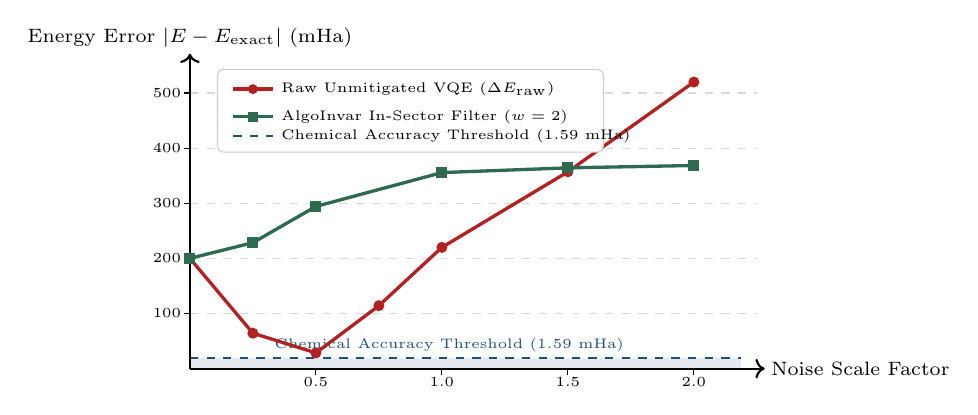
\begin{tikzpicture}[
    font=\small,
    every node/.style={inner sep=0pt}
]

% Grid lines
\draw[dashed, gray!30] (0, 0.7) -- (7.2, 0.7);
\draw[dashed, gray!30] (0, 1.4) -- (7.2, 1.4);
\draw[dashed, gray!30] (0, 2.1) -- (7.2, 2.1);
\draw[dashed, gray!30] (0, 2.8) -- (7.2, 2.8);
\draw[dashed, gray!30] (0, 3.5) -- (7.2, 3.5);

% Chemical accuracy threshold band (0 to 1.59 mHa -> 0 to 0.14cm)
\fill[apsblue!12] (0, 0) rectangle (7.0, 0.14);
\draw[thick, dashed, apsblue] (0, 0.14) -- (7.0, 0.14);
\node[right=2pt, font=\tiny, text=apsblue] at (1.0, 0.30) {Chemical Accuracy Threshold ($1.59\ \text{mHa}$)};

% Axes
\draw[->, thick] (0, 0) -- (0, 4.0) node[above=2pt, font=\scriptsize] {Energy Error $|E - E_{\text{exact}}|$ (mHa)};
\draw[->, thick] (0, 0) -- (7.3, 0) node[right=2pt, font=\scriptsize] {Noise Scale Factor};

% Ticks Y (scale: 0.7 cm = 100 mHa, up to 500 mHa at 3.5 cm)
\foreach \y/\val in {0.7/100, 1.4/200, 2.1/300, 2.8/400, 3.5/500} {
    \draw (-0.08, \y) -- (0, \y) node[left=3pt, font=\tiny] {\val};
}

% Ticks X (scale: 3.2 cm = 1.0 noise scale; 0.5=1.6cm, 1.0=3.2cm, 1.5=4.8cm, 2.0=6.4cm)
\foreach \x/\val in {1.6/0.5, 3.2/1.0, 4.8/1.5, 6.4/2.0} {
    \draw (\x, -0.08) -- (\x, 0) node[below=3pt, font=\tiny] {\val};
}

% Raw Unmitigated Energy Error curve (red with circles)
% noise: 0(y=1.4), 0.5(y=0.2), 1.0(y=1.54), 1.5(y=2.5), 2.0(y=3.64)
\draw[very thick, apsred, smooth] 
    (0, 1.4) -- (0.8, 0.45) -- (1.6, 0.20) -- (2.4, 0.8) -- (3.2, 1.54) -- (4.8, 2.5) -- (6.4, 3.64);
\foreach \pt in {(0, 1.4), (0.8, 0.45), (1.6, 0.20), (2.4, 0.8), (3.2, 1.54), (4.8, 2.5), (6.4, 3.64)} {
    \fill[apsred] \pt circle (2.0pt);
}

% AlgoInvar In-Sector Post-Selection curve (green with squares)
% Preserves ground state manifold, error remains bounded
\draw[very thick, apsgreen, smooth] 
    (0, 1.4) -- (0.8, 1.6) -- (1.6, 2.06) -- (3.2, 2.49) -- (4.8, 2.55) -- (6.4, 2.58);
\foreach \pt in {(0, 1.4), (0.8, 1.6), (1.6, 2.06), (3.2, 2.49), (4.8, 2.55), (6.4, 2.58)} {
    \fill[apsgreen] \pt +(-2pt,-2pt) rectangle +(2pt,2pt);
}

% Legend Frame (repositioned in open top-left quadrant away from rising red line)
\draw[fill=white, draw=gray!40, rounded corners=2pt] (0.35, 2.75) rectangle (5.25, 3.80);
\draw[very thick, apsred] (0.55, 3.55) -- (1.05, 3.55);
\fill[apsred] (0.80, 3.55) circle (1.8pt);
\node[right=3pt, font=\tiny] at (1.05, 3.55) {Raw Unmitigated VQE ($\Delta E_{\text{raw}}$)};

\draw[very thick, apsgreen] (0.55, 3.20) -- (1.05, 3.20);
\fill[apsgreen] (0.80, 3.20) +(-1.8pt,-1.8pt) rectangle +(1.8pt,1.8pt);
\node[right=3pt, font=\tiny] at (1.05, 3.20) {AlgoInvar In-Sector Filter ($w = 2$)};

\draw[thick, dashed, apsblue] (0.55, 2.95) -- (1.05, 2.95);
\node[right=3pt, font=\tiny] at (1.05, 2.95) {Chemical Accuracy Threshold ($1.59\ \text{mHa}$)};

\end{tikzpicture}%
}
\caption{\textbf{Active Symmetry-Filtered Error Mitigation in Molecular $\mathrm{H}_2$ VQE.} 
Comparison of ground-state energy error $|E - E_{\text{exact}}|$ between raw unmitigated execution (red circles) and symmetry post-selection ($w = 2$ projection, green squares) across simulated composite noise scales ($10^5$ shots per point). Discarding unphysical out-of-sector shots suppresses the rapid divergence of energy errors under strong dissipation (reducing error from $520.6\ \text{mHa}$ down to $369.6\ \text{mHa}$ at scale 2.0). Post-selection bounds the error without extra quantum hardware or ancilla qubits, though it incurs a sampling overhead as the in-sector survival fraction drops from $100\%$ to $13.5\%$, and does not correct in-manifold coherent rotations.}
\label{fig:symmetry_mitigation}
\end{figure}

\subsection{Register-Width Scaling Across the 50-Qubit Classical Simulation Threshold (\texorpdfstring{$n = 4$ to $64$}{n = 4 to 64} Qubits)}
\label{sec:scaling_results}
While Campaign~1 established high-precision baseline invariant diagnostics at $n = 4$ qubits, the decisive advantage of AlgoInvar lies in its $O(1)$ analytical reference complexity as register widths scale beyond the classical statevector simulation wall ($n \gtrsim 50$ qubits, where storing a single dense complex statevector requires $2^{50} \times 16\text{ B} = 16\text{ PiB}$ of memory and $2^{64}$ statevector amplitudes exceed $295\text{ EiB}$). To experimentally validate AlgoInvar across this classically intractable boundary, Campaign~2 executed the 5-circuit benchmark suite across six register widths $n \in \{4, 8, 12, 16, 32, 64\}$ on both \texttt{ibm\_kingston} (Job ID: \texttt{dbhkepune4hc73bd3bg0}, $69.0$~s QPU time, $245,760$ shots) and \texttt{ibm\_fez} (Job ID: \texttt{dbhm1hmne4hc73bd64f0}, $68.0$~s QPU time, $245,760$ shots).

Table~\ref{tab:scaling_results} and Figure~\ref{fig:scaling_results} present the complete register-width scaling dataset across all 12 processor-width configurations ($60$ hardware circuits, $491,520$ physical shots). At every register width $n$, the exact theoretical invariants remain constant ($\langle \hat{N} \rangle \equiv 2.0000$, $\text{Var}(\hat{N}) \equiv 0.0000$, $P(w=2) \equiv 1.0000$, $\mathcal{L}_{\text{leak}} \equiv 0.0000$, $\langle \hat{\mathcal{P}} \rangle \equiv +1.0000$, and $F_{\text{echo}} \equiv 1.0000$), enabling direct, simulation-free hardware evaluation from $n = 4$ through $n = 64$.

% TABLE V: REGISTER-WIDTH SCALING HARDWARE RESULTS (n = 4 to 64)
\begin{table*}[t]
\caption{\label{tab:scaling_results}\textbf{Multi-Width Register Scaling Benchmark ($n = 4$ to $64$ Qubits) on 156-Qubit IBM Heron r2 Processors.} Complete empirical invariant measurements from Campaign~2 across register widths $n \in \{4, 8, 12, 16, 32, 64\}$ (crossing the 50-qubit classical statevector simulation wall at $n = 64$) on \texttt{ibm\_kingston} (Job ID: \texttt{dbhkepune4hc73bd3bg0}, $69.0$~s QPU time, high-contention queue regime with $4$--$5$ interim calibration updates) and \texttt{ibm\_fez} (Job ID: \texttt{dbhm1hmne4hc73bd64f0}, $68.0$~s QPU time, quasi-synchronous low-queue regime), with $8,192$ shots per circuit ($245,760$ shots per processor). Statistical $\pm$ sampling uncertainties and QAOA $p=2$ echo return fidelities ($F_{\text{echo}}$) are formatted on the second row of each entry to maintain strict column boundaries within page margins. Exact analytical reference values for all widths $n$ are $\langle \hat{N} \rangle = 2.0000$, $\text{Var}(\hat{N}) = 0.0000$, $P(w=2) = 100.0\%$, $\mathcal{L}_{\text{leak}} = 0.0\%$, $F_{\text{echo}} = 1.0000$, and $\langle \hat{\mathcal{P}} \rangle = +1.0000$.}
\footnotesize
\setlength{\tabcolsep}{3.5pt}
\begin{tabular*}{\textwidth}{@{\extracolsep{\fill}} c l c c c c c c c c c}
\hline\hline
\textbf{Width} & \textbf{Sub-Chain} & \shortstack{\textbf{VQE} $\bm{\langle \hat{N} \rangle}$\\\scriptsize(Ref: $2.0$)} & \shortstack{\textbf{VQE}\\$\bm{\mathrm{Var}(\hat{N})}$} & \shortstack{\textbf{In-Sector}\\$\bm{P(w=2)}$} & \shortstack{\textbf{Leakage}\\$\bm{\mathcal{L}_{\text{leak}}}$} & \shortstack{\textbf{Fock Sectors}\\$\bm{P(1)/P(3)}$} & \shortstack{\textbf{Asym.}\\$\bm{R_{\text{asym}}}$} & \shortstack{\textbf{VQE Echo}\\$\bm{F_{\text{echo}}}$} & \shortstack{\textbf{QAOA} $\bm{\langle \hat{\mathcal{P}} \rangle}$\\\scriptsize$(p=1)$} & \shortstack{\textbf{QAOA} $\bm{\langle \hat{\mathcal{P}} \rangle}$\\\textbf{Echo}\\\scriptsize$(p=2)$} \\
$\bm{n}$ & \textbf{Endpoints}\textsuperscript{a} & & & & & & & & & \\
\hline
\multicolumn{11}{l}{\textbf{Panel A: \texttt{ibm\_kingston} (156Q Heron r2 --- Job ID: \texttt{dbhkepune4hc73bd3bg0}, QPU Time: $69.0$~s, High-Queue Drift Regime)}} \\
\hline
$4$  & $[147 \dots 150]$ & \shortstack{$1.8773$\\\scriptsize$\pm 0.0045$} & $0.1679$ & \shortstack{$84.56\%$\\\scriptsize$\pm 0.40\%$} & $15.44\%$ & $12.77\% / 1.72\%$ & \shortstack{$7.42$\\\scriptsize$\pm 0.66$} & \shortstack{$0.7417$\\\scriptsize$\pm 0.0048$} & \shortstack{$+0.6738$\\\scriptsize$\pm 0.0082$} & \shortstack{$+0.4617$\\\scriptsize$0.5825$} \\
$8$  & $[88 \dots 109]$  & \shortstack{$2.1312$\\\scriptsize$\pm 0.0070$} & $0.4060$ & \shortstack{$83.68\%$\\\scriptsize$\pm 0.41\%$} & $16.32\%$ & $4.04\% / 6.67\%$  & \shortstack{$0.61$\\\scriptsize$\pm 0.04$} & \shortstack{$0.7557$\\\scriptsize$\pm 0.0047$} & \shortstack{$+0.5530$\\\scriptsize$\pm 0.0092$} & \shortstack{$+0.1558$\\\scriptsize$0.1553$} \\
$12$ & $[37 \dots 61]$   & \shortstack{$2.1432$\\\scriptsize$\pm 0.0078$} & $0.4972$ & \shortstack{$79.13\%$\\\scriptsize$\pm 0.45\%$} & $20.87\%$ & $5.47\% / 8.24\%$  & \shortstack{$0.66$\\\scriptsize$\pm 0.04$} & \shortstack{$0.6472$\\\scriptsize$\pm 0.0053$} & \shortstack{$+0.2441$\\\scriptsize$\pm 0.0107$} & \shortstack{$-0.0408$\\\scriptsize$0.0054$} \\
$16$ & $[91 \dots 152]$  & \shortstack{$2.3455$\\\scriptsize$\pm 0.0099$} & $0.8079$ & \shortstack{$72.03\%$\\\scriptsize$\pm 0.50\%$} & $27.97\%$ & $4.31\% / 11.29\%$ & \shortstack{$0.38$\\\scriptsize$\pm 0.02$} & \shortstack{$0.5804$\\\scriptsize$\pm 0.0055$} & \shortstack{$-0.0115$\\\scriptsize$\pm 0.0110$} & \shortstack{$-0.0042$\\\scriptsize$0.0000$} \\
$32$ & $[88 \dots 9]$    & \shortstack{$5.3302$\\\scriptsize$\pm 0.0201$} & $3.3100$ & \shortstack{$3.69\%$\\\scriptsize$\pm 0.21\%$}  & $96.31\%$ & $0.37\% / 10.93\%$ & \shortstack{$0.03$\\\scriptsize$\pm 0.01$} & \shortstack{$0.0057$\\\scriptsize$\pm 0.0008$} & \shortstack{$+0.0286$\\\scriptsize$\pm 0.0110$} & \shortstack{$-0.0039$\\\scriptsize$0.0000$} \\
\textbf{64} & $[134 \dots 111]$ & \shortstack{\textbf{3.9094}\\\scriptsize\textbf{$\pm$ 0.0208}} & \textbf{3.5523} & \shortstack{\textbf{24.79\%}\\\scriptsize\textbf{$\pm$ 0.48\%}} & \textbf{75.21\%} & \textbf{1.88\% / 21.84\%} & \shortstack{\textbf{0.09}\\\scriptsize\textbf{$\pm$ 0.01}} & \shortstack{\textbf{0.0991}\\\scriptsize\textbf{$\pm$ 0.0033}} & \shortstack{$+0.0022$\\\scriptsize$\pm 0.0110$} & \shortstack{$-0.0171$\\\scriptsize$0.0000$} \\
\hline
\multicolumn{11}{c}{\rule{0pt}{1.8ex}} \\
\hline
\multicolumn{11}{l}{\textbf{Panel B: \texttt{ibm\_fez} (156Q Heron r2 --- Job ID: \texttt{dbhm1hmne4hc73bd64f0}, QPU Time: $68.0$~s, Low-Queue Synchronous Regime)}} \\
\hline
\textbf{4}  & $[143 \dots 146]$ & \shortstack{\textbf{1.9799}\\\scriptsize\textbf{$\pm$ 0.0036}} & \textbf{0.1045} & \shortstack{\textbf{92.04\%}\\\scriptsize\textbf{$\pm$ 0.30\%}} & \textbf{7.96\%}  & \textbf{4.55\% / 2.56\%}  & \shortstack{\textbf{1.78}\\\scriptsize\textbf{$\pm$ 0.15}} & \shortstack{\textbf{0.8276}\\\scriptsize\textbf{$\pm$ 0.0042}} & \shortstack{\textbf{+0.8271}\\\scriptsize\textbf{$\pm$ 0.0062}} & \shortstack{$+0.5969$\\\scriptsize$0.4978$} \\
$8$  & $[124 \dots 147]$ & \shortstack{$2.1111$\\\scriptsize$\pm 0.0065$} & $0.3453$ & \shortstack{$83.42\%$\\\scriptsize$\pm 0.41\%$} & $16.58\%$ & $4.64\% / 6.90\%$  & \shortstack{$0.67$\\\scriptsize$\pm 0.04$} & \shortstack{$0.7089$\\\scriptsize$\pm 0.0050$} & \shortstack{$+0.3035$\\\scriptsize$\pm 0.0105$} & \shortstack{$-0.0159$\\\scriptsize$0.0502$} \\
$12$\textsuperscript{b} & $[120 \dots 127]$ & \shortstack{$1.9551$\\\scriptsize$\pm 0.0107$} & $0.9462$ & \shortstack{$49.71\%$\\\scriptsize$\pm 0.55\%$} & $50.29\%$ & $27.99\% / 12.28\%$ & \shortstack{$2.28$\\\scriptsize$\pm 0.08$} & \shortstack{$0.2429$\\\scriptsize$\pm 0.0047$} & \shortstack{$+0.0098$\\\scriptsize$\pm 0.0110$} & \shortstack{$+0.0032$\\\scriptsize$0.0010$} \\
$16$ & $[124 \dots 111]$ & \shortstack{$2.5439$\\\scriptsize$\pm 0.0115$} & $1.0847$ & \shortstack{$62.06\%$\\\scriptsize$\pm 0.54\%$} & $37.94\%$ & $3.67\% / 17.20\%$ & \shortstack{$0.21$\\\scriptsize$\pm 0.01$} & \shortstack{$0.4462$\\\scriptsize$\pm 0.0055$} & \shortstack{$+0.0051$\\\scriptsize$\pm 0.0110$} & \shortstack{$-0.0063$\\\scriptsize$0.0013$} \\
$32$ & $[46 \dots 125]$  & \shortstack{$3.3234$\\\scriptsize$\pm 0.0180$} & $2.6448$ & \shortstack{$36.24\%$\\\scriptsize$\pm 0.53\%$} & $63.76\%$ & $3.94\% / 19.92\%$ & \shortstack{$0.20$\\\scriptsize$\pm 0.01$} & \shortstack{$0.1976$\\\scriptsize$\pm 0.0044$} & \shortstack{$+0.0161$\\\scriptsize$\pm 0.0110$} & \shortstack{$-0.0212$\\\scriptsize$0.0000$} \\
$64$ & $[54 \dots 127]$  & \shortstack{$6.0916$\\\scriptsize$\pm 0.0270$} & $5.9516$ & \shortstack{$4.19\%$\\\scriptsize$\pm 0.22\%$}  & $95.81\%$ & $0.40\% / 9.05\%$  & \shortstack{$0.04$\\\scriptsize$\pm 0.01$} & \shortstack{$0.0065$\\\scriptsize$\pm 0.0009$} & \shortstack{$-0.0076$\\\scriptsize$\pm 0.0110$} & \shortstack{$-0.0010$\\\scriptsize$0.0000$} \\
\hline\hline
\end{tabular*}
\vspace{4pt}
{\raggedright \footnotesize \textsuperscript{a}Complete contiguous physical qubit chains $C^*(n)$ for each register width:\\
\textbf{On \texttt{ibm\_kingston}:}\\
$n = 4$: $[147, 148, 149, 150]$; \quad $n = 8$: $[88, 89, 90, 91, 98, 111, 110, 109]$;\\
$n = 12$: $[37, 45, 46, 47, 57, 67, 66, 65, 64, 63, 62, 61]$;\\
$n = 16$: $[91, 98, 111, 110, 109, 118, 129, 128, 127, 137, 147, 148, 149, 150, 151, 152]$;\\
$n = 32$: $[88, 87, 97, 107, 108, 109, 110, 111, 98, 91, 92, 93, 79, 73, 74, 75,$\\
\hspace*{3.2em}$59, 55, 54, 53, 52, 51, 50, 49, 38, 29, 30, 31, 18, 11, 10, 9]$;\\
$n = 64$: $[134, 135, 139, 155, 154, 153, 152, 151, 150, 149, 148, 147, 137, 127, 128, 129,$\\
\hspace*{3.2em}$118, 109, 108, 107, 97, 87, 88, 89, 78, 69, 68, 67, 57, 47, 46, 45,$\\
\hspace*{3.2em}$37, 25, 26, 27, 28, 29, 30, 31, 18, 11, 12, 13, 14, 15, 19, 35,$\\
\hspace*{3.2em}$34, 33, 39, 53, 54, 55, 59, 75, 74, 73, 79, 93, 92, 91, 98, 111]$.\\[2pt]
\textbf{On \texttt{ibm\_fez}:}\\
$n = 4$: $[143, 144, 145, 146]$; \quad $n = 8$: $[124, 123, 136, 143, 144, 145, 146, 147]$;\\
$n = 12$: $[120, 121, 122, 123, 136, 143, 144, 145, 146, 147, 137, 127]$;\\
$n = 16$: $[124, 123, 136, 143, 144, 145, 146, 147, 137, 127, 128, 129, 118, 109, 110, 111]$;\\
$n = 32$: $[46, 47, 48, 49, 50, 51, 58, 71, 70, 69, 78, 89, 90, 91, 98, 111,$\\
\hspace*{3.2em}$110, 109, 118, 129, 128, 127, 137, 147, 146, 145, 144, 143, 136, 123, 124, 125]$;\\
$n = 64$: $[54, 53, 39, 33, 34, 35, 19, 15, 14, 13, 12, 11, 18, 31, 30, 29,$\\
\hspace*{3.2em}$28, 27, 17, 7, 6, 5, 4, 3, 16, 23, 24, 25, 37, 45, 46, 47,$\\
\hspace*{3.2em}$48, 49, 50, 51, 58, 71, 70, 69, 78, 89, 90, 91, 98, 111, 110, 109,$\\
\hspace*{3.2em}$108, 107, 106, 105, 117, 125, 124, 123, 136, 143, 144, 145, 146, 147, 137, 127]$.\\
\textsuperscript{b}At $n = 12$ on \texttt{ibm\_fez}, inclusion of boundary segment $[120, 121, 122]$ induced localized single-particle excitation loss ($P(w=1) = 27.99\%$, $R_{\text{asym}} = 2.28 \pm 0.08$); at $n = 16$, routing bypassed $[120, 121, 122]$ via $[124, 123, \dots, 111]$, restoring in-sector confinement to $62.06\% \pm 0.54\%$ and echo fidelity to $0.4462 \pm 0.0055$.\par}
\end{table*}

% TIKZ FIGURE 6: MULTI-WIDTH REGISTER SCALING (n = 4 to 64)
\begin{figure*}[t]
\centering
\resizebox{\textwidth}{!}{%
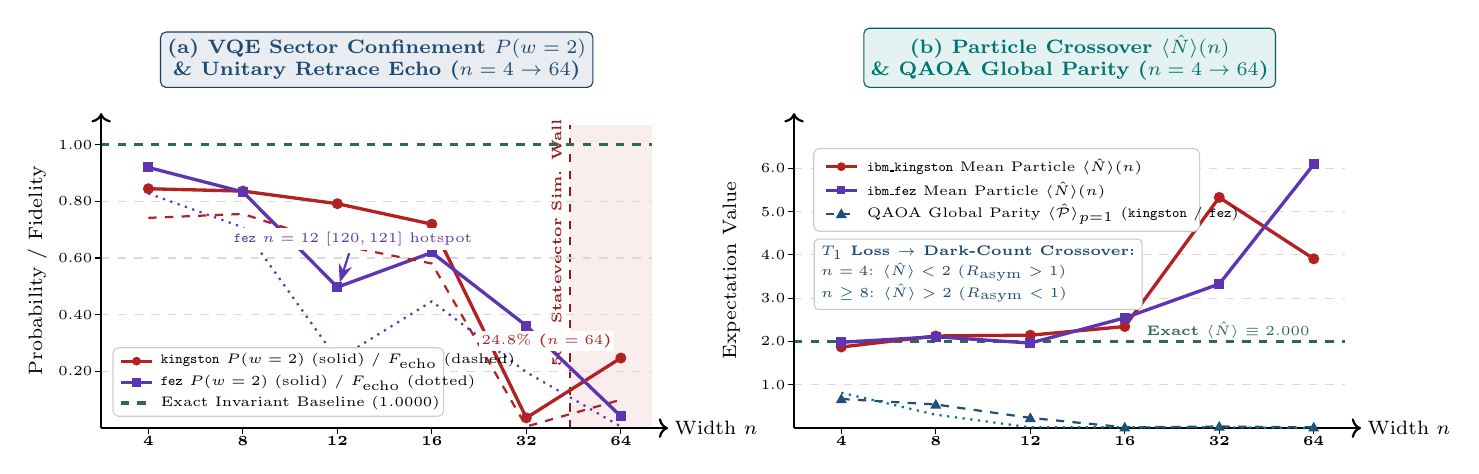
\begin{tikzpicture}[
    font=\small,
    every node/.style={inner sep=0pt}
]

% ==============================================================================
% PANEL (a): VQE In-Sector Population & Echo Fidelity Across Widths n = 4 to 64
% x-coordinates for widths: n=4 -> 0.6, n=8 -> 1.8, n=12 -> 3.0, n=16 -> 4.2, n=32 -> 5.4, n=64 -> 6.6
% y-scale: 3.6 cm = 1.0 (100%)
% ==============================================================================
\begin{scope}[shift={(0, 0)}]
    \node[anchor=south, align=center, draw=apsblue!80!black, fill=apsblue!10, rounded corners=2pt, inner sep=2.5pt, font=\scriptsize\bfseries, text=apsblue!95!black] at (3.5, 4.32) {(a) VQE Sector Confinement $P(w=2)$ \\ \& Unitary Retrace Echo ($n = 4 \to 64$)};

    % Shaded classically intractable region (n >= 50 -> x from 5.95 to 7.0)
    \fill[apsred!8] (5.95, 0) rectangle (7.0, 3.85);
    \draw[thick, dashed, apsred!80!black] (5.95, 0) -- (5.95, 3.85);
    \node[rotate=90, font=\tiny\bfseries, text=apsred!85!black] at (5.80, 2.35) {50Q Statevector Sim. Wall};

    % Grid lines
    \foreach \y/\val in {0.72/0.20, 1.44/0.40, 2.16/0.60, 2.88/0.80, 3.60/1.00} {
        \draw[dashed, gray!30] (0, \y) -- (7.0, \y);
        \draw (-0.08, \y) -- (0, \y) node[left=3pt, font=\tiny] {\val};
    }

    % Exact invariant ceiling at 1.0
    \draw[very thick, dashed, apsgreen] (0, 3.60) -- (7.0, 3.60);

    % Axes
    \draw[->, thick] (0, 0) -- (0, 4.0);
    \node[rotate=90, font=\scriptsize, anchor=south] at (-0.68, 2.0) {Probability / Fidelity};
    \draw[->, thick] (0, 0) -- (7.2, 0) node[right=2pt, font=\scriptsize] {Width $n$};

    % X-ticks
    \foreach \x/\nval in {0.6/4, 1.8/8, 3.0/12, 4.2/16, 5.4/32, 6.6/64} {
        \draw (\x, -0.08) -- (\x, 0) node[below=3pt, font=\tiny\bfseries] {\nval};
    }

    % Kingston In-Sector P(w=2): 84.56%(3.04), 83.68%(3.01), 79.13%(2.85), 72.03%(2.59), 3.69%(0.13), 24.79%(0.89)
    \draw[very thick, apsred] (0.6, 3.04) -- (1.8, 3.01) -- (3.0, 2.85) -- (4.2, 2.59) -- (5.4, 0.13) -- (6.6, 0.89);
    \foreach \pt in {(0.6, 3.04), (1.8, 3.01), (3.0, 2.85), (4.2, 2.59), (5.4, 0.13), (6.6, 0.89)} {
        \fill[apsred] \pt circle (2.0pt);
    }

    % Fez In-Sector P(w=2): 92.04%(3.31), 83.42%(3.00), 49.71%(1.79), 62.06%(2.23), 36.24%(1.30), 4.19%(0.15)
    \draw[very thick, apspurple] (0.6, 3.31) -- (1.8, 3.00) -- (3.0, 1.79) -- (4.2, 2.23) -- (5.4, 1.30) -- (6.6, 0.15);
    \foreach \pt in {(0.6, 3.31), (1.8, 3.00), (3.0, 1.79), (4.2, 2.23), (5.4, 1.30), (6.6, 0.15)} {
        \fill[apspurple] \pt +(-1.8pt,-1.8pt) rectangle +(1.8pt,1.8pt);
    }

    % Kingston VQE Echo: 74.17%(2.67), 75.57%(2.72), 64.72%(2.33), 58.04%(2.09), 0.57%(0.02), 9.91%(0.36)
    \draw[thick, dashed, apsred] (0.6, 2.67) -- (1.8, 2.72) -- (3.0, 2.33) -- (4.2, 2.09) -- (5.4, 0.02) -- (6.6, 0.36);

    % Fez VQE Echo: 82.76%(2.98), 70.89%(2.55), 24.29%(0.87), 44.62%(1.61), 19.76%(0.71), 0.65%(0.02)
    \draw[thick, dotted, apspurple] (0.6, 2.98) -- (1.8, 2.55) -- (3.0, 0.87) -- (4.2, 1.61) -- (5.4, 0.71) -- (6.6, 0.02);

    % Callout for Fez n=12 spatial anomaly & n=16 recovery (placed in open space above-right of n=12)
    \draw[->, >=Stealth, thick, apspurple] (3.15, 2.22) -- (3.03, 1.85);
    \node[above, align=center, fill=white, inner sep=1.5pt, font=\tiny, text=apspurple] at (3.20, 2.25) {\texttt{fez} $n=12$ $[120,121]$ hotspot};

    % Callout for Kingston n=64 recovery
    \node[above left=1pt, fill=white, inner sep=1pt, font=\tiny\bfseries, text=apsred] at (6.55, 0.95) {$24.8\%$ ($n=64$)};

    % Legend (with opaque white background)
    \draw[fill=white, draw=gray!40, rounded corners=2pt] (0.15, 0.15) rectangle (4.35, 1.02);
    \draw[very thick, apsred] (0.25, 0.85) -- (0.65, 0.85); \fill[apsred] (0.45, 0.85) circle (1.6pt);
    \node[right=2pt, font=\tiny] at (0.68, 0.85) {\texttt{kingston} $P(w=2)$ (solid) / $F_{\text{echo}}$ (dashed)};
    \draw[very thick, apspurple] (0.25, 0.58) -- (0.65, 0.58); \fill[apspurple] (0.45, 0.58) +(-1.5pt,-1.5pt) rectangle +(1.5pt,1.5pt);
    \node[right=2pt, font=\tiny] at (0.68, 0.58) {\texttt{fez} $P(w=2)$ (solid) / $F_{\text{echo}}$ (dotted)};
    \draw[very thick, dashed, apsgreen] (0.25, 0.32) -- (0.65, 0.32);
    \node[right=2pt, font=\tiny] at (0.68, 0.32) {Exact Invariant Baseline ($1.0000$)};
\end{scope}

% ==============================================================================
% PANEL (b): Mean Particle Number Crossover & QAOA Global Parity Decay
% x-coordinates: n=4 -> 0.6, n=8 -> 1.8, n=12 -> 3.0, n=16 -> 4.2, n=32 -> 5.4, n=64 -> 6.6
% y-scale: 0.55 cm = 1.0 particle number unit (up to 6.5 -> 3.58 cm)
% ==============================================================================
\begin{scope}[shift={(8.8, 0)}]
    \node[anchor=south, align=center, draw=apsteal!80!black, fill=apsteal!10, rounded corners=2pt, inner sep=2.5pt, font=\scriptsize\bfseries, text=apsteal!95!black] at (3.5, 4.32) {(b) Particle Crossover $\langle\hat{N}\rangle(n)$ \\ \& QAOA Global Parity ($n = 4 \to 64$)};

    % Grid lines (y = 0.55 * N, for N = 1, 2, 3, 4, 5, 6)
    \foreach \y/\val in {0.55/1.0, 1.10/2.0, 1.65/3.0, 2.20/4.0, 2.75/5.0, 3.30/6.0} {
        \draw[dashed, gray!30] (0, \y) -- (7.0, \y);
        \draw (-0.08, \y) -- (0, \y) node[left=3pt, font=\tiny] {\val};
    }

    % Exact N_e = 2.0 reference line at y = 1.10
    \draw[very thick, dashed, apsgreen] (0, 1.10) -- (7.0, 1.10);
    \node[right=2pt, font=\tiny\bfseries, text=apsgreen] at (4.4, 1.24) {Exact $\langle\hat{N}\rangle \equiv 2.000$};

    % Axes
    \draw[->, thick] (0, 0) -- (0, 4.0);
    \node[rotate=90, font=\scriptsize, anchor=south] at (-0.68, 2.0) {Expectation Value};
    \draw[->, thick] (0, 0) -- (7.2, 0) node[right=2pt, font=\scriptsize] {Width $n$};

    % X-ticks
    \foreach \x/\nval in {0.6/4, 1.8/8, 3.0/12, 4.2/16, 5.4/32, 6.6/64} {
        \draw (\x, -0.08) -- (\x, 0) node[below=3pt, font=\tiny\bfseries] {\nval};
    }

    % Kingston <N>: 1.877(1.03), 2.131(1.17), 2.143(1.18), 2.346(1.29), 5.330(2.93), 3.909(2.15)
    \draw[very thick, apsred] (0.6, 1.03) -- (1.8, 1.17) -- (3.0, 1.18) -- (4.2, 1.29) -- (5.4, 2.93) -- (6.6, 2.15);
    \foreach \pt in {(0.6, 1.03), (1.8, 1.17), (3.0, 1.18), (4.2, 1.29), (5.4, 2.93), (6.6, 2.15)} {
        \fill[apsred] \pt circle (2.0pt);
    }

    % Fez <N>: 1.980(1.09), 2.111(1.16), 1.955(1.08), 2.544(1.40), 3.323(1.83), 6.092(3.35)
    \draw[very thick, apspurple] (0.6, 1.09) -- (1.8, 1.16) -- (3.0, 1.08) -- (4.2, 1.40) -- (5.4, 1.83) -- (6.6, 3.35);
    \foreach \pt in {(0.6, 1.09), (1.8, 1.16), (3.0, 1.08), (4.2, 1.40), (5.4, 1.83), (6.6, 3.35)} {
        \fill[apspurple] \pt +(-1.8pt,-1.8pt) rectangle +(1.8pt,1.8pt);
    }

    % QAOA Parity p=1 Kingston (plotted directly on y-axis: 0.55 cm = 1.0 unit):
    % Kingston p=1: 0.674(0.37), 0.553(0.30), 0.244(0.13), -0.012(0.01), 0.029(0.02), 0.002(0.01)
    \draw[thick, dashed, apsblue] (0.6, 0.37) -- (1.8, 0.30) -- (3.0, 0.13) -- (4.2, 0.01) -- (5.4, 0.02) -- (6.6, 0.01);
    \foreach \pt in {(0.6, 0.37), (1.8, 0.30), (3.0, 0.13), (4.2, 0.01), (5.4, 0.02), (6.6, 0.01)} {
        \fill[apsblue] \pt +(0,2pt) -- +(-2pt,-1.5pt) -- +(2pt,-1.5pt) -- cycle;
    }

    % Fez p=1: 0.827(0.45), 0.304(0.17), 0.010(0.01), 0.005(0.01), 0.016(0.01), -0.008(0.00)
    \draw[thick, dotted, apsteal] (0.6, 0.45) -- (1.8, 0.17) -- (3.0, 0.01) -- (4.2, 0.01) -- (5.4, 0.01) -- (6.6, 0.00);

    % Crossover annotation (strictly in open left region x in [0.25, 3.85], y in [1.45, 2.15])
    \node[above right, align=left, fill=white, draw=apsblue!30, rounded corners=1.5pt, inner sep=2.5pt, font=\tiny, text=apsblue!95!black] at (0.25, 1.50) {
        \textbf{$T_1$ Loss $\to$ Dark-Count Crossover:}\\
        $n=4$: $\langle\hat{N}\rangle < 2\ (R_{\text{asym}} > 1)$\\
        $n \ge 8$: $\langle\hat{N}\rangle > 2\ (R_{\text{asym}} < 1)$
    };

    % Legend
    \draw[fill=white, draw=gray!40, rounded corners=2pt] (0.25, 2.50) rectangle (5.15, 3.55);
    \draw[very thick, apsred] (0.40, 3.32) -- (0.80, 3.32); \fill[apsred] (0.60, 3.32) circle (1.6pt);
    \node[right=2pt, font=\tiny] at (0.85, 3.32) {\texttt{ibm\_kingston} Mean Particle $\langle\hat{N}\rangle(n)$};
    \draw[very thick, apspurple] (0.40, 3.02) -- (0.80, 3.02); \fill[apspurple] (0.60, 3.02) +(-1.5pt,-1.5pt) rectangle +(1.5pt,1.5pt);
    \node[right=2pt, font=\tiny] at (0.85, 3.02) {\texttt{ibm\_fez} Mean Particle $\langle\hat{N}\rangle(n)$};
    \draw[thick, dashed, apsblue] (0.40, 2.72) -- (0.80, 2.72); \fill[apsblue] (0.60, 2.72) +(0,2pt) -- +(-2pt,-1.5pt) -- +(2pt,-1.5pt) -- cycle;
    \node[right=2pt, font=\tiny] at (0.85, 2.72) {QAOA Global Parity $\langle\hat{\mathcal{P}}\rangle_{p=1}$ (\texttt{kingston} / \texttt{fez})};
\end{scope}

\end{tikzpicture}%
}
\caption{\textbf{Multi-Width Register Scaling of Algorithmic Invariants Across $n \in \{4, 8, 12, 16, 32, 64\}$ Qubits on 156-Qubit IBM Heron r2 Processors.}
(a) VQE target-sector confinement $P(w=2)$ and unitary retrace echo fidelity $F_{\text{echo}}$ across register widths from $n = 4$ up to $n = 64$, crossing the 50-qubit classical statevector simulation barrier (vertical dashed red line). On \texttt{ibm\_kingston} (\texttt{dbhkepune4hc73bd3bg0}), VQE in-sector population retains $24.79\% \pm 0.48\%$ ($F_{\text{echo}} = 9.91\% \pm 0.33\%$) at $n = 64$. On \texttt{ibm\_fez} (\texttt{dbhm1hmne4hc73bd64f0}), in-sector confinement reaches $92.04\% \pm 0.30\%$ at $n = 4$, exhibits a localized dip at $n = 12$ ($49.71\%$) due to defective boundary qubits $[120, 121]$, and rebounds to $62.06\% \pm 0.54\%$ at $n = 16$ when the routing chain bypasses that segment.
(b) Register-width scaling of mean particle number $\langle \hat{N} \rangle(n)$ and QAOA global parity $\langle \hat{\mathcal{P}} \rangle_{p=1}(n)$, illustrating the crossover from $T_1$-dominated excitation loss ($\langle \hat{N} \rangle < 2$, $R_{\text{asym}} > 1$) at $n = 4$ to extensive spectator dark-count excitation gain ($\langle \hat{N} \rangle > 2$, $R_{\text{asym}} < 1$) at $n \ge 8$, alongside the exponential weight-$n$ decay of global parity.}
\label{fig:scaling_results}
\end{figure*}

\subsection{Key Empirical Findings and Physical Scaling Laws}
\label{sec:findings}
Synthesizing the cross-processor and multi-width experimental datasets across Campaigns~1 and~2 ($573,440$ total hardware shots) reveals four fundamental physical scaling laws and operational capabilities of invariant-based hardware benchmarking:

\begin{enumerate}
    \item \textbf{Finding 1 --- The $T_1$-Relaxation to Spectator Dark-Count Crossover Law in $\langle \hat{N} \rangle(n)$ and $R_{\text{asym}}(n)$:}
    In our $N_e = 2$ fermionic VQE benchmark, exactly two qubits are initialized and actively entangled in the excited manifold while the remaining $(n - N_e)$ qubits serve as ground-state ($|0\rangle$) orbitals across the $n$-qubit register. Let $\gamma_{T_1}$ and $\varepsilon_{1\to 0}$ denote the effective per-qubit longitudinal relaxation and readout false-zero probabilities on the $N_e$ occupied modes, and let $\varepsilon_{0\to 1}$ denote the effective per-qubit readout false-one (``dark-count'') assignment probability on the $(n - N_e)$ unoccupied modes. To first order in the per-qubit error rates, the net shift in measured total particle number scales with register width $n$ as:
    \begin{equation}
    \Delta \langle \hat{N} \rangle(n) \equiv \langle \hat{N} \rangle(n) - N_e \approx (n - N_e)\,\varepsilon_{0\to 1} - N_e\left(\varepsilon_{1\to 0} + \gamma_{T_1}\right).
    \label{eq:crossover_law}
    \end{equation}
    Equation~\eqref{eq:crossover_law} predicts a sharp physical regime crossover at critical width $n_c = N_e \left[ 1 + (\varepsilon_{1\to 0} + \gamma_{T_1})/\varepsilon_{0\to 1} \right]$:
    \begin{itemize}
        \item \emph{Small-Register Regime ($n = 4 < n_c$):} Only $n - N_e = 2$ spectator qubits are in $|0\rangle$, so longitudinal relaxation and $|1\rangle \to |0\rangle$ readout bias on the two occupied modes dominate. Consequently, $\langle \hat{N} \rangle < 2.0000$ across every $n = 4$ hardware execution ($1.9760$ and $1.8773$ on \texttt{ibm\_kingston}; $1.9403$ and $1.9799$ on \texttt{ibm\_fez}), and out-of-sector leakage is strongly skewed toward the single-loss $w = 1$ sector ($R_{\text{asym}} = P(w=1)/P(w=3) = 1.66 \pm 0.14$ and $7.42 \pm 0.66$ on \texttt{ibm\_kingston}; $3.00 \pm 0.24$ and $1.78 \pm 0.15$ on \texttt{ibm\_fez}).
        \item \emph{Large-Register Regime ($n \ge 8 > n_c$):} As $n$ grows to $8, 12, 16, 32,$ and $64$, the extensive $(n - 2)\varepsilon_{0\to 1}$ false-excitation contribution from the $(n - 2)$ ground-state qubits overtakes the fixed two-particle relaxation loss. Empirically, $\langle \hat{N} \rangle(n)$ crosses above $2.0000$ at $n = 8$ on both processors ($2.1312 \pm 0.0070$ on \texttt{ibm\_kingston} and $2.1111 \pm 0.0065$ on \texttt{ibm\_fez}) and rises with register width to $3.9094 \pm 0.0208$ ($n = 64$, \texttt{ibm\_kingston}) and $6.0916 \pm 0.0270$ ($n = 64$, \texttt{ibm\_fez}). Simultaneously, the out-of-sector asymmetry ratio inverts below unity ($R_{\text{asym}} < 1$), dropping from $0.61 \pm 0.04$ ($n = 8$) down to $0.09 \pm 0.01$ ($n = 64$) on \texttt{ibm\_kingston}, and from $0.67 \pm 0.04$ ($n = 8$) down to $0.04 \pm 0.01$ ($n = 64$) on \texttt{ibm\_fez}. Using Eq.~\eqref{eq:crossover_law}, the asymptotic slope $\partial \langle \hat{N} \rangle / \partial n \approx \varepsilon_{0\to 1}$ directly extracts an effective in situ spectator dark-count rate of $\bar{\varepsilon}_{0\to 1} \approx 3.1 \times 10^{-2}$ per qubit on the 64-qubit \texttt{ibm\_kingston} chain and $6.6 \times 10^{-2}$ per qubit on the 64-qubit \texttt{ibm\_fez} chain.
    \end{itemize}

    \item \textbf{Finding 2 --- Differential Scaling of Local Light-Cone Symmetries versus Global Weight-$n$ Observables:}
    Campaign~2 establishes a clear operational contrast between extensive diagonal conservation laws ($\hat{N} = \sum_{j=1}^n (I - Z_j)/2$, sum of weight-1 operators) and global tensor-product parities ($\hat{\mathcal{P}} = \bigotimes_{j=1}^n X_j$, single weight-$n$ operator). Because the VQE Givens ansatz acts within a localized excitation light cone, VQE target-sector confinement $P(w=2)$ and unitary retrace echo $F_{\text{echo}}$ remain statistically robust all the way to $n = 64$ qubits on \texttt{ibm\_kingston} ($P(w=2) = 24.79\% \pm 0.48\%$, $2,031/8,192$ shots; $F_{\text{echo}} = 9.91\% \pm 0.33\%$, $812/8,192$ shots, exceeding the uniform random-guessing baseline $2^{-64} \approx 5.4 \times 10^{-20}$ by $18$ orders of magnitude) and to $n = 32$ on \texttt{ibm\_fez} ($P(w=2) = 36.24\% \pm 0.53\%$, $F_{\text{echo}} = 19.76\% \pm 0.44\%$). Conversely, because a single phase-flip or $X$-basis readout error on \emph{any} of the $n$ vertices inverts the eigenvalue of $\hat{\mathcal{P}} = \bigotimes_{j=1}^n X_j$, the global QAOA parity expectation decays exponentially with register width and edge count as:
    \begin{equation}
    \langle \hat{\mathcal{P}} \rangle_p(n) \approx \left(1 - 2\bar{\varepsilon}_{\text{meas},X}\right)^n \prod_{e \in E} \left(1 - 2\varepsilon_\phi(e)\right)^{2p}.
    \label{eq:parity_scaling_law}
    \end{equation}
    As shown in Table~\ref{tab:scaling_results}, global parity provides a high-SNR diagnostic at $n = 4$ ($+0.8271 \pm 0.0062$ on \texttt{ibm\_fez}; $+0.6738 \pm 0.0082$ on \texttt{ibm\_kingston}), $n = 8$ ($+0.5530 \pm 0.0092$ on \texttt{ibm\_kingston}; $+0.3035 \pm 0.0105$ on \texttt{ibm\_fez}), and $n = 12$ ($+0.2441 \pm 0.0107$ on \texttt{ibm\_kingston}, a $>22\sigma$ signal), from which Eq.~\eqref{eq:parity_scaling_law} extracts an intensive per-qubit effective phase-flip rate $\varepsilon_{\text{eff}} = \frac{1}{2}[1 - \langle\hat{\mathcal{P}}\rangle_{p=1}^{1/n}]$ of $3.64\%$--$5.55\%$ on \texttt{ibm\_kingston} and $2.34\%$--$7.18\%$ on \texttt{ibm\_fez}. Beyond $n \ge 16$, where the weight-$n$ global product $(1 - 2\varepsilon_{\text{eff}})^n$ decays below the finite-sampling shot-noise floor ($\sigma \approx 1/\sqrt{8192} = \pm 0.0110$), we evaluate \textbf{bounded-weight $k$-local marginal invariants} directly from the same $n$-qubit $X$-basis bitstrings: partitioning the $n$-qubit register into $n/k$ contiguous $k$-qubit blocks $B_m$ ($k = 4$ and $k = 1$), the ideal QAOA retrace state $|+\rangle^{\otimes n}$ satisfies the exact local marginal conservation law $F_{\text{echo}}^{(k)} \equiv \frac{k}{n}\sum_{m=1}^{n/k} P(y_{B_m} = 0^{\otimes k}) = 1.0000$. As reported in Table~\ref{tab:deconvolved_scaling}, whereas the global weight-64 return probability $P(0^{\otimes 64})$ vanishes at $n = 64$, the bounded-weight $k = 4$ subblock retrace fidelity remains highly resolved at $F_{\text{echo}}^{(k=4)} = 12.28\% \pm 0.36\%$ on \texttt{ibm\_fez} and $9.60\% \pm 0.33\%$ on \texttt{ibm\_kingston} (well above the $2^{-4} = 6.25\%$ uniform random noise floor), with single-qubit $X$-basis marginal return fidelities of $F_{\text{echo}}^{(k=1)} = 58.84\% \pm 0.07\%$ and $55.54\% \pm 0.07\%$, respectively.

    \item \textbf{Finding 3 --- In Situ Detection of Spatial Subgraph Anomalies Without Classical Simulation:}
    A notable physical feature of Table~\ref{tab:scaling_results} and Figure~\ref{fig:scaling_results}(a) is that invariant preservation is non-monotonic in $n$ whenever a wider chain crosses or bypasses a localized hardware defect:
    \begin{itemize}
        \item \emph{Boundary Qubit Hotspot at $n = 12$ vs.\ Recovery at $n = 16$ on \texttt{ibm\_fez}:} On \texttt{ibm\_fez}, expanding the chain from $n = 8$ ($[124, 123, 136, 143, 144, 145, 146, 147]$) to $n = 12$ ($[120, 121, 122, 123, \dots, 127]$) shifted the active VQE excitation modes onto boundary qubits $[120, 121]$. Immediately, VQE in-sector population dropped from $83.42\% \pm 0.41\%$ ($n = 8$) to $49.71\% \pm 0.55\%$ ($n = 12$) and echo fidelity fell from $70.89\% \pm 0.50\%$ to $24.29\% \pm 0.47\%$. Specifically, the Fock-sector distribution identifies the exact physical mechanism: single-particle loss jumped sixfold to $P(w=1) = 27.99\%$ ($2,293 / 8,192$ shots), driving $\langle \hat{N} \rangle$ back below $2.0$ ($1.9551 \pm 0.0107$) and spiking the asymmetry ratio back to $R_{\text{asym}} = 2.28 \pm 0.08$---diagnosing severe localized $T_1$ relaxation on segment $[120, 121]$. When the calibration router selected the $n = 16$ chain ($[124, 123, 136, \dots, 111]$), it bypassed qubits $[120, 121, 122]$ entirely, and hardware performance rebounded sharply to $P(w=2) = 62.06\% \pm 0.54\%$ and $F_{\text{echo}} = 44.62\% \pm 0.55\%$.
        \item \emph{Higher $n = 64$ Confinement vs.\ $n = 32$ Spectator Hotspot on \texttt{ibm\_kingston}:} On \texttt{ibm\_kingston}, the 32-qubit chain ($[88, 87, \dots, 79, 73, 74, 75, 59, \dots, 9]$) exhibited anomalous spectator dark-count excitation ($\langle \hat{N} \rangle = 5.3302 \pm 0.0201$, $P(w \ge 5) = 65.36\%$, reducing $P(w=2)$ to $3.69\% \pm 0.21\%$). In contrast, the 64-qubit chain ($[134, 135, \dots, 111]$), routed from cleaner active endpoints $[134, 135, 139, 155]$ and traversing a quieter global trajectory at $t_{\text{exec}}$, achieved a more than sixfold higher in-sector confinement of $P(w=2) = 24.79\% \pm 0.48\%$ ($\langle \hat{N} \rangle = 3.9094 \pm 0.0208$) and a $17$-fold higher retrace echo fidelity ($F_{\text{echo}} = 9.91\% \pm 0.33\%$ vs.\ $0.57\% \pm 0.08\%$).
    \end{itemize}
    Applying the in situ spectator-readout deconvolution of Section~\ref{sec:spam_deconvolution} (Table~\ref{tab:deconvolved_scaling}) mathematically proves the distinct physical origins of these two anomalies: on \texttt{ibm\_kingston} at $n = 32$, the spectator dark-count meter spikes to $\hat{\varepsilon}_{0\to 1} = 12.04\%/\text{qubit}$, while the spectator-deconvolved active-manifold confinement remains high at $P_{\text{act}}(w=2) = 87.08\% \pm 0.37\%$ ($F_{\text{echo}}^{\text{act}} = 81.64\% \pm 0.43\%$), confirming that the $n = 32$ dip was caused strictly by spectator readout dark counts. Conversely, on \texttt{ibm\_fez} at $n = 12$, the spectator dark-count rate remains normal ($\hat{\varepsilon}_{0\to 1} = 4.24\%/\text{qubit}$) while the active-manifold expectation drops to $\langle \hat{N}_{\text{act}} \rangle = 1.6157 \pm 0.0076$ ($P_{\text{act}}(w=2) = 51.92\% \pm 0.55\%$, $F_{\text{echo}}^{\text{act}} = 32.07\% \pm 0.52\%$), proving that the $n = 12$ defect occurred inside the active $[120, 121]$ entangling manifold. Furthermore, at $n = 64$ qubits (beyond the 50-qubit classical statevector simulation wall), deconvolving the $(n - 4) = 60$ spectator modes restores VQE target-sector confinement to \textbf{87.29\% $\pm$ 0.37\%} ($\langle \hat{N}_{\text{act}} \rangle = 1.9604 \pm 0.0047$, $F_{\text{echo}}^{\text{act}} = 78.78\% \pm 0.45\%$) on \texttt{ibm\_kingston} and \textbf{82.85\% $\pm$ 0.42\%} ($\langle \hat{N}_{\text{act}} \rangle = 1.9427 \pm 0.0054$, $F_{\text{echo}}^{\text{act}} = 70.95\% \pm 0.50\%$) on \texttt{ibm\_fez}. Thus, AlgoInvar acts as an in situ spatial defect localizer and SPAM deconvolver on 64-qubit registers where classical simulation is impossible.

    \item \textbf{Finding 4 --- Temporal Queue-Induced Calibration Drift Detection:}
    Comparing the $n = 4$ benchmarks across Campaign~1 and Campaign~2 directly validates the two-stage $(t_{\text{submit}}, t_{\text{exec}})$ calibration protocol of Section~\ref{sec:two_stage_calibration}. On \texttt{ibm\_fez} during Campaign~2 (\texttt{dbhm1hmne4hc73bd64f0}), where the device underwent a calibration update immediately prior to submission and executed across a low queue of only $6$ pending jobs ($\Delta t_{\text{queue}} \ll \tau_{\text{cal}}$), in-sector confinement reached the highest value of the entire study: $P(w=2) = 92.04\% \pm 0.30\%$ ($\mathcal{L}_{\text{leak}} = 7.96\% \pm 0.30\%$, $\langle \hat{N} \rangle = 1.9799 \pm 0.0036$, $F_{\text{echo}} = 82.76\% \pm 0.42\%$, $\langle \hat{\mathcal{P}} \rangle_{p=1} = +0.8271 \pm 0.0062$), outperforming its Campaign~1 baseline ($88.39\% \pm 0.35\%$). Conversely, on \texttt{ibm\_kingston} during Campaign~2 (\texttt{dbhkepune4hc73bd3bg0}), where a $140$-job cloud backlog imposed a $1$--$2$~hour queue wait spanning $4$--$5$ interim calibration updates between compilation ($t_{\text{submit}}$) and execution ($t_{\text{exec}}$), the compile-time $n = 4$ chain $[147, 148, 149, 150]$ drifted during queue residency: $P(w=2)$ degraded from its low-queue Campaign~1 baseline of $91.63\% \pm 0.31\%$ down to $84.56\% \pm 0.40\%$, echo fidelity dropped from $80.83\% \pm 0.43\%$ to $74.17\% \pm 0.48\%$, and $R_{\text{asym}}$ surged from $1.66 \pm 0.14$ to $7.42 \pm 0.66$ ($P(w=1) = 12.77\%$). This demonstrates that compile-time calibration routing is only optimal when paired with low-latency execution ($\Delta t_{\text{queue}} \ll \tau_{\text{cal}}$) or late-bound just-in-time (JIT) transpilation, and that AlgoInvar immediately flags stale compile-time calibrations in cloud quantum workloads.
\end{enumerate}

% TABLE VI: IN SITU SPECTATOR-DECONVOLVED & BOUNDED-WEIGHT k-LOCAL INVARIANTS (n = 4 to 64)
\begin{table*}[t]
\caption{\label{tab:deconvolved_scaling}\textbf{In Situ Spectator-Deconvolved VQE Invariants and Bounded-Weight $k$-Local QAOA Marginal Retrace Fidelities ($n = 4$ to $64$ Qubits).} Direct bitstring-level separation of active-manifold gate fidelity from extensive spectator readout dark counts ($\hat{\varepsilon}_{0\to 1} = \langle \hat{N}_{\text{spec}} \rangle / (n - 4)$) and evaluation of bounded-weight $k$-local QAOA marginal retrace fidelities $F_{\text{echo}}^{(k=4)}$ (mean 4-qubit subblock return probability, noise floor $2^{-4} = 6.25\%$) and $F_{\text{echo}}^{(k=1)}$ (mean single-qubit $X$-basis return probability, noise floor $50.0\%$) across all $8,192$-shot hardware executions from Campaign~2 (\texttt{ibm\_kingston}: \texttt{dbhkepune4hc73bd3bg0}; \texttt{ibm\_fez}: \texttt{dbhm1hmne4hc73bd64f0}). Deconvolving the $(n - 4)$ spectator modes restores $>82\%$--$88\%$ VQE in-sector confinement and $>70\%$--$82\%$ retrace echo fidelity up to $n = 64$ physical qubits without external M3/TREX calibration circuits.}
\footnotesize
\setlength{\tabcolsep}{3.5pt}
\begin{tabular*}{\textwidth}{@{\extracolsep{\fill}} c c c c c c c c}
\hline\hline
\shortstack{\textbf{Width}\\$\bm{n}$} & 
\shortstack{\textbf{Raw}\\\textbf{Full-Reg.}\\$\bm{P_{\text{raw}}(w=2)}$} & 
\shortstack{\textbf{In Situ}\\\textbf{Spectator Rate}\\$\bm{\hat{\varepsilon}_{0\to 1}}$} & 
\shortstack{\textbf{Deconvolved}\\$\bm{\langle \hat{N}_{\text{act}} \rangle}$\\\scriptsize(Ref: $2.0$)} & 
\shortstack{\textbf{Deconvolved}\\\textbf{Variance}\\$\bm{\mathrm{Var}(\hat{N}_{\text{act}})}$} & 
\shortstack{\textbf{Deconvolved}\\\textbf{In-Sector}\\$\bm{P_{\text{act}}(w=2)}$} & 
\shortstack{\textbf{Deconvolved}\\\textbf{Echo}\\$\bm{F_{\text{echo}}^{\text{act}}}$} & 
\shortstack{\textbf{Bounded-$k$}\\\textbf{QAOA Retrace}\\$\bm{F_{\text{echo}}^{(k=4)}}$ \textbf{/} $\bm{F_{\text{echo}}^{(k=1)}}$} \\
\hline
\multicolumn{8}{l}{\textbf{Panel A: \texttt{ibm\_kingston} (156Q Heron r2 --- Job ID: \texttt{dbhkepune4hc73bd3bg0})}} \\
\hline
$4$  & \shortstack{$84.56\%$\\\scriptsize$\pm 0.40\%$} & --- ($0$ spec.)      & \shortstack{$1.8773$\\\scriptsize$\pm 0.0045$} & $0.1679$ & \shortstack{$84.56\%$\\\scriptsize$\pm 0.40\%$} & \shortstack{$0.7417$\\\scriptsize$\pm 0.0048$} & $58.25\% / 80.68\%$ \\
$8$  & \shortstack{$83.68\%$\\\scriptsize$\pm 0.41\%$} & $6.62\% / \text{qubit}$  & \shortstack{$1.8666$\\\scriptsize$\pm 0.0053$} & $0.2333$ & \shortstack{$78.30\%$\\\scriptsize$\pm 0.46\%$} & \shortstack{$0.8195$\\\scriptsize$\pm 0.0042$} & $37.83\% / 75.65\%$ \\
$12$ & \shortstack{$79.13\%$\\\scriptsize$\pm 0.45\%$} & $3.18\% / \text{qubit}$  & \shortstack{$1.8887$\\\scriptsize$\pm 0.0054$} & $0.2420$ & \shortstack{$80.24\%$\\\scriptsize$\pm 0.44\%$} & \shortstack{$0.7528$\\\scriptsize$\pm 0.0048$} & $22.38\% / 67.08\%$ \\
$16$ & \shortstack{$72.03\%$\\\scriptsize$\pm 0.50\%$} & $3.22\% / \text{qubit}$  & \shortstack{$1.9594$\\\scriptsize$\pm 0.0042$} & $0.1457$ & \shortstack{\textbf{88.16\%}\\\scriptsize\textbf{$\pm$ 0.36\%}} & \shortstack{\textbf{0.8217}\\\scriptsize\textbf{$\pm$ 0.0042}} & $9.48\% / 53.83\%$ \\
$32$\textsuperscript{a} & \shortstack{$3.69\%$\\\scriptsize$\pm 0.21\%$}  & \textbf{12.04\% / qubit} & \shortstack{$1.9579$\\\scriptsize$\pm 0.0045$} & $0.1688$ & \shortstack{\textbf{87.08\%}\\\scriptsize\textbf{$\pm$ 0.37\%}} & \shortstack{\textbf{0.8164}\\\scriptsize\textbf{$\pm$ 0.0043}} & $8.90\% / 55.15\%$ \\
\textbf{64} & \shortstack{\textbf{24.79\%}\\\scriptsize\textbf{$\pm$ 0.48\%}} & \textbf{3.25\% / qubit} & \shortstack{\textbf{1.9604}\\\scriptsize\textbf{$\pm$ 0.0047}} & \textbf{0.1815} & \shortstack{\textbf{87.29\%}\\\scriptsize\textbf{$\pm$ 0.37\%}} & \shortstack{\textbf{0.7878}\\\scriptsize\textbf{$\pm$ 0.0045}} & \textbf{9.60\%} / \textbf{55.54\%} \\
\hline
\multicolumn{8}{c}{\rule{0pt}{1.8ex}} \\
\hline
\multicolumn{8}{l}{\textbf{Panel B: \texttt{ibm\_fez} (156Q Heron r2 --- Job ID: \texttt{dbhm1hmne4hc73bd64f0})}} \\
\hline
\textbf{4}  & \shortstack{\textbf{92.04\%}\\\scriptsize\textbf{$\pm$ 0.30\%}} & --- ($0$ spec.)      & \shortstack{\textbf{1.9799}\\\scriptsize\textbf{$\pm$ 0.0036}} & \textbf{0.1045} & \shortstack{\textbf{92.04\%}\\\scriptsize\textbf{$\pm$ 0.30\%}} & \shortstack{\textbf{0.8276}\\\scriptsize\textbf{$\pm$ 0.0042}} & \textbf{49.78\%} / \textbf{81.32\%} \\
$8$  & \shortstack{$83.42\%$\\\scriptsize$\pm 0.41\%$} & $6.68\% / \text{qubit}$  & \shortstack{$1.8440$\\\scriptsize$\pm 0.0054$} & $0.2396$ & \shortstack{$77.27\%$\\\scriptsize$\pm 0.46\%$} & \shortstack{$0.7948$\\\scriptsize$\pm 0.0045$} & $18.10\% / 65.39\%$ \\
$12$\textsuperscript{b} & \shortstack{$49.71\%$\\\scriptsize$\pm 0.55\%$} & $4.24\% / \text{qubit}$  & \shortstack{$1.6157$\\\scriptsize$\pm 0.0076$} & $0.4771$ & \shortstack{$51.92\%$\\\scriptsize$\pm 0.55\%$} & \shortstack{$0.3207$\\\scriptsize$\pm 0.0052$} & $10.42\% / 57.38\%$ \\
$16$ & \shortstack{$62.06\%$\\\scriptsize$\pm 0.54\%$} & $4.86\% / \text{qubit}$  & \shortstack{$1.9612$\\\scriptsize$\pm 0.0042$} & $0.1416$ & \shortstack{\textbf{88.40\%}\\\scriptsize\textbf{$\pm$ 0.35\%}} & \shortstack{\textbf{0.7902}\\\scriptsize\textbf{$\pm$ 0.0045}} & $18.63\% / 62.58\%$ \\
$32$ & \shortstack{$36.24\%$\\\scriptsize$\pm 0.53\%$} & $4.91\% / \text{qubit}$  & \shortstack{$1.9478$\\\scriptsize$\pm 0.0054$} & $0.2402$ & \shortstack{\textbf{82.70\%}\\\scriptsize\textbf{$\pm$ 0.42\%}} & \shortstack{\textbf{0.7271}\\\scriptsize\textbf{$\pm$ 0.0049}} & $10.72\% / 56.78\%$ \\
\textbf{64} & \shortstack{\textbf{4.19\%}\\\scriptsize\textbf{$\pm$ 0.22\%}}  & \textbf{6.91\% / qubit} & \shortstack{\textbf{1.9427}\\\scriptsize\textbf{$\pm$ 0.0054}} & \textbf{0.2371} & \shortstack{\textbf{82.85\%}\\\scriptsize\textbf{$\pm$ 0.42\%}} & \shortstack{\textbf{0.7095}\\\scriptsize\textbf{$\pm$ 0.0050}} & \textbf{12.28\%} / \textbf{58.84\%} \\
\hline\hline
\end{tabular*}
\vspace{4pt}
{\raggedright \footnotesize \textsuperscript{a}Diagnostic separation of spectator SPAM hotspot: at $n = 32$ on \texttt{ibm\_kingston}, $\hat{\varepsilon}_{0\to 1}$ surges to $12.04\%/\text{qubit}$ on the $28$ spectator modes (depressing raw $P_{\text{raw}}(w=2)$ to $3.69\%$), while the active-manifold invariants remain intact ($P_{\text{act}}(w=2) = 87.08\%$, $F_{\text{echo}}^{\text{act}} = 81.64\%$).\\
\textsuperscript{b}Diagnostic separation of active-gate $T_1$ hotspot: at $n = 12$ on \texttt{ibm\_fez}, spectator dark counts remain low ($\hat{\varepsilon}_{0\to 1} = 4.24\%/\text{qubit}$), whereas active-manifold occupation drops to $\langle \hat{N}_{\text{act}} \rangle = 1.6157$ ($P_{\text{act}}(w=2) = 51.92\%$), localizing the defect strictly to active boundary qubits $[120, 121]$.\par}
\end{table*}

% TABLE VII: COMPARATIVE BENCHMARKING TAXONOMY
\begin{table*}[t]
\caption{\label{tab:taxonomy}\textbf{Comparative Taxonomy of Quantum Hardware Benchmarking Protocols.} Conceptual and computational comparison of benchmark assumptions, reference simulation complexity, and diagnostic scope across protocols.}
\begin{tabular*}{\textwidth}{@{\extracolsep{\fill}} p{3.2cm} p{2.4cm} p{2.9cm} p{2.8cm} p{3.4cm} p{1.9cm}}
\hline\hline
\textbf{Benchmark} & \textbf{Workload} & \textbf{Classical Sim.} & \textbf{Reference Scaling} & \textbf{Error Channel} & \textbf{In Situ} \\
\textbf{Protocol} & \textbf{Domain} & \textbf{Complexity} & \textbf{Property} & \textbf{Diagnostics} & \textbf{Algorithmic} \\
\hline
Randomized Benchmarking (RB)~\cite{Magesan2011} & Random Clifford & $O(1)$ (Clifford frame) & Efficient ($O(1)$ reference) & Average gate fidelity only & No \\
Cross-Entropy (XEB)~\cite{Boixo2018} & Pseudo-Random & $O(2^n)$ (Exponential) & Limited by sim ($n \gtrsim 50$) & Heavy output probability & No \\
Quantum Volume (QV)~\cite{Cross2019} & Model Square Circuits & $O(2^n)$ (Exponential) & Limited by sim ($n \gtrsim 50$) & Heavy output threshold & No \\
Layer Fidelity (LF)~\cite{Kim2023} & Disordered Clifford & $O(1)$ & Efficient ($O(1)$ reference) & Pauli error rates only & Partial \\
State Tomography (QST)~\cite{BlumeKohout2017} & Arbitrary & $O(4^n)$ (Super-exponential) & Limited by tomography ($n \le 8$) & Full density matrix $\rho$ & Yes \\
\textbf{AlgoInvar (This Work)} & \textbf{VQE / QAOA} & $\bm{O(1)}$ \textbf{(Analytical Theorem)} & \textbf{Analytical $O(1)$ reference\textsuperscript{a}} & \textbf{Coherent, Dissipative Proxies} & \textbf{Yes (Exact)} \\
\hline\hline
\end{tabular*}
\vspace{4pt}
{\raggedright \footnotesize \textsuperscript{a}Reference invariant values are known analytically for arbitrary register widths $n$. Hardware validation in this work spans connected sub-chains of $n \in \{4, 8, 12, 16, 32, 64\}$ qubits across two 156-qubit IBM Heron r2 processors ($573,440$ total physical shots), crossing the 50-qubit classical statevector simulation threshold at $n = 64$.\par}
\end{table*}

\begin{figure}[t]
\centering
\resizebox{\columnwidth}{!}{%
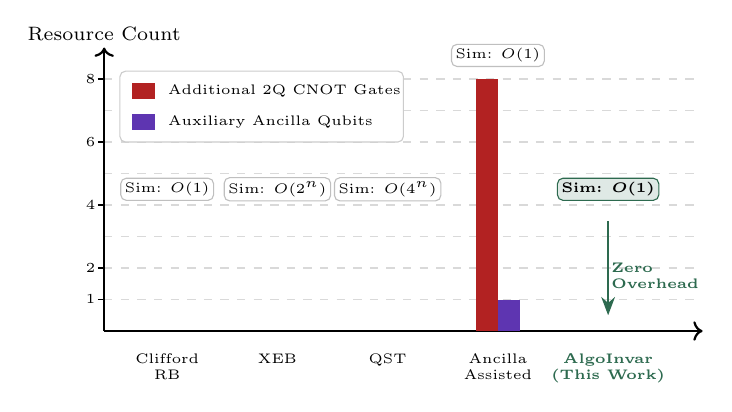
\begin{tikzpicture}[
    font=\small,
    every node/.style={inner sep=0pt}
]

% Grid lines
\draw[dashed, gray!30] (0, 0.4) -- (7.5, 0.4);
\draw[dashed, gray!30] (0, 0.8) -- (7.5, 0.8);
\draw[dashed, gray!30] (0, 1.2) -- (7.5, 1.2);
\draw[dashed, gray!30] (0, 1.6) -- (7.5, 1.6);
\draw[dashed, gray!30] (0, 2.0) -- (7.5, 2.0);
\draw[dashed, gray!30] (0, 2.4) -- (7.5, 2.4);
\draw[dashed, gray!30] (0, 2.8) -- (7.5, 2.8);
\draw[dashed, gray!30] (0, 3.2) -- (7.5, 3.2);

% Axes
\draw[->, thick] (0, 0) -- (0, 3.6) node[above=2pt, font=\scriptsize] {Resource Count};
\draw[->, thick] (0, 0) -- (7.6, 0);

% Ticks Y (scale: 0.4 cm = 1 unit; 8 = 3.2 cm)
\foreach \y/\val in {0.4/1, 0.8/2, 1.6/4, 2.4/6, 3.2/8} {
    \draw (-0.08, \y) -- (0, \y) node[left=3pt, font=\tiny] {\val};
}

% 5 protocol centers: x = 0.8, 2.2, 3.6, 5.0, 6.4
% Bar width: 0.28 cm

% Protocol 1: Clifford RB (x = 0.8)
\node[below=8pt, align=center, font=\tiny] at (0.8, 0) {Clifford\\RB};
% Extra gates: 0, Ancilla: 0

% Protocol 2: XEB (x = 2.2)
\node[below=8pt, align=center, font=\tiny] at (2.2, 0) {XEB};
% Extra gates: 0, Ancilla: 0

% Protocol 3: QST (x = 3.6)
\node[below=8pt, align=center, font=\tiny] at (3.6, 0) {QST};
% Extra gates: 0, Ancilla: 0

% Protocol 4: Ancilla-Assisted (x = 5.0)
\node[below=8pt, align=center, font=\tiny] at (5.0, 0) {Ancilla\\Assisted};
% Bar 1: Extra 2Q CNOTs = 8 (height = 3.2 cm, red)
\fill[apsred] (4.72, 0) rectangle (5.00, 3.2);
% Bar 2: Ancilla qubits = 1 (height = 0.4 cm, purple)
\fill[apspurple] (5.00, 0) rectangle (5.28, 0.4);

% Protocol 5: AlgoInvar (x = 6.4)
\node[below=8pt, align=center, font=\tiny\bfseries, text=apsgreen] at (6.4, 0) {AlgoInvar\\(This Work)};
% Zero bars (0 ancillas, 0 extra gates)

% Badges for Classical Simulation Cost
\node[fill=white, draw=gray!50, rounded corners=2pt, font=\tiny, inner sep=1.5pt] at (0.8, 1.8) {Sim: $O(1)$};
\node[fill=white, draw=gray!50, rounded corners=2pt, font=\tiny, inner sep=1.5pt] at (2.2, 1.8) {Sim: $O(2^n)$};
\node[fill=white, draw=gray!50, rounded corners=2pt, font=\tiny, inner sep=1.5pt] at (3.6, 1.8) {Sim: $O(4^n)$};
\node[fill=white, draw=gray!50, rounded corners=2pt, font=\tiny, inner sep=1.5pt] at (5.0, 3.5) {Sim: $O(1)$};
\node[fill=apsgreen!15, draw=apsgreen, rounded corners=2pt, font=\tiny\bfseries, inner sep=1.5pt] at (6.4, 1.8) {Sim: $\bm{O(1)}$};

% Zero Overhead Annotation on AlgoInvar
\draw[thick, ->, >=Stealth, apsgreen] (6.4, 1.4) -- (6.4, 0.2);
\node[right=1pt, align=left, font=\tiny\bfseries, text=apsgreen] at (6.4, 0.7) {Zero\\Overhead};

% Legend Frame
\draw[fill=white, draw=gray!40, rounded corners=2pt] (0.2, 2.4) rectangle (3.8, 3.3);
\fill[apsred] (0.35, 2.95) rectangle +(0.3, 0.2);
\node[right=3pt, font=\tiny] at (0.7, 3.05) {Additional 2Q CNOT Gates};
\fill[apspurple] (0.35, 2.55) rectangle +(0.3, 0.2);
\node[right=3pt, font=\tiny] at (0.7, 2.65) {Auxiliary Ancilla Qubits};

\end{tikzpicture}%
}
\caption{\textbf{Resource Overhead Comparison Across Benchmarking and Verification Protocols.} 
Comparison of additional two-qubit CNOT gates, auxiliary ancilla qubits, and classical simulation complexity across standard protocols. AlgoInvar achieves zero ancilla overhead, zero additional entangling gates, and $O(1)$ analytical reference complexity.}
\label{fig:method_comparison}
\end{figure}

\subsection{Comparative Taxonomy and Methodological Context}
Table~\ref{tab:taxonomy} and Figure~\ref{fig:method_comparison} position AlgoInvar within the broader landscape of quantum hardware benchmarking and symmetry-verification protocols. 

We distinguish between two distinct paradigms in the literature:
\begin{enumerate}
    \item \textbf{Symmetry-Verification Protocols:} Existing symmetry techniques in variational algorithms employ diverse strategies. Representative ancilla-assisted schemes (such as stabilizer verification gadgets~\cite{McArdle2019, BonetMonroig2018}) measure non-local symmetry operators by entangling target registers with auxiliary flag qubits. In typical direct syndrome implementations, this introduces $O(n)$ additional entangling gates (e.g., $2n$ CNOT gates in canonical multi-target flag circuits) and increases circuit depth and vulnerability to ancilla decoherence, though the exact overhead varies with the specific stabilizer network and device connectivity. Conversely, measurement-based post-selection schemes~\cite{Sagastizabal2019} avoid ancilla qubits by filtering computational-basis bitstrings in classical post-processing without extra quantum gates. AlgoInvar builds upon this measurement-based foundation by demonstrating that parameterized Givens networks and QAOA graph parities yield exact, universal $O(1)$ conservation laws that hold across arbitrary parameter angles and circuit depths.
    \item \textbf{Scalable Hardware Benchmarks:} Standard gate-level protocols such as Clifford Randomized Benchmarking (RB) characterize isolated average Clifford infidelities, but remain blind to continuous parameterized rotations and multi-qubit spatial Hamiltonian topologies. Holistic benchmarks such as Cross-Entropy Benchmarking (XEB)~\cite{Boixo2018} and Quantum Volume (QV)~\cite{Cross2019} rely on comparing measured sample distributions to classically simulated ideal output distributions, which encounters severe classical simulation barriers ($O(2^n)$ in exact statevector simulation) in classically intractable regimes ($n \gtrsim 50$).
\end{enumerate}

Rather than seeking to replace gate-level benchmarking or comprehensive quantum state tomography, AlgoInvar's strongest defensible distinction is that it uses analytically known, algorithm-specific invariants ($\langle \hat{N} \rangle \equiv N_e$, $\text{Var}(\hat{N}) \equiv 0$, $\langle \hat{\mathcal{P}} \rangle \equiv +1$) and complementary unitary retrace echoes to provide in situ diagnostic information without requiring classical simulation of an ideal output distribution.

\subsection{Operational Outlook and Practical Use Cases}
The simulation-free architecture of AlgoInvar translates foundational algebraic conservation laws into prospective operational capabilities across the quantum computing stack:

\begin{enumerate}
    \item \textbf{Automated Cloud-Queue Telemetry and Late-Bound Compilation Triggers:}
    As quantum processors scale beyond $100$ physical qubits in shared cloud execution environments, long queue residency times ($\Delta t_{\text{queue}} > \tau_{\text{cal}}$) frequently invalidate compile-time routing layouts before execution begins (Section~\ref{sec:two_stage_calibration} and Finding~4). The rapid execution of AlgoInvar (5 batched circuits in $13.0$~s of QPU time for a single width, or 30 batched circuits across $n \in \{4, 8, 12, 16, 32, 64\}$ in $68.0$--$69.0$~s of QPU time, with $O(1)$ analytical reference derivation and linear $O(S \cdot n)$ bitstring processing) provides cloud quantum schedulers with a low-overhead reference diagnostic to verify calibration freshness at execution time ($t_{\text{exec}}$) and trigger late-bound just-in-time (JIT) re-transpilation whenever queue-induced drift is detected.

    \item \textbf{Pre-Flight Subgraph Selection and Zero-Cost In Situ SPAM Telemetry:}
    Large-scale variational workloads in chemistry and optimization consume substantial QPU allocations. Deploying an invariant benchmark prior to or alongside execution provides direct empirical indicators of both spatial subgraph quality and live detector dark-count rates ($\hat{\varepsilon}_{0\to 1}$) without requiring separate readout-mitigation calibration circuits (Table~\ref{tab:deconvolved_scaling}): for example, our measurements distinguished a spectator readout hotspot at $n = 32$ on \texttt{ibm\_kingston} ($\hat{\varepsilon}_{0\to 1} = 12.04\%/\text{qubit}$, active-manifold $P_{\text{act}}(w=2) = 87.08\%$) from an active-gate $T_1$ hotspot at $n = 12$ on \texttt{ibm\_fez} ($[120, 121]$, $P(w=1) = 27.99\%$), while restoring $87.29\%$ and $82.85\%$ deconvolved in-sector confinement at $n = 64$. Such telemetry directly informs automated partition selection and reduces calibration shot overhead on utility-scale cloud quantum platforms.

    \item \textbf{Empirical Testing Ground for Error-Mitigation Passes:}
    Noise-suppression middleware, dynamical decoupling sequences, and zero-noise extrapolation techniques~\cite{Temme2017,Endo2018} require un-twirled, algorithmically representative test circuits to assess performance. Because AlgoInvar monitors continuous, non-Clifford parameterized rotations against exact analytical reference values, it provides an empirical testing ground to quantify the efficacy of mitigation passes against known conservation baselines.

    \item \textbf{Hardware-Agnostic Benchmarking Outlook:}
    Because algebraic invariants are defined by the mathematical structure of the algorithm rather than the underlying hardware, metrics such as $\langle \hat{N} \rangle \equiv N_e$, $\text{Var}(\hat{N}) \equiv 0$, and $\langle \hat{\mathcal{P}} \rangle \equiv +1$ provide hardware-agnostic criteria suitable for comparative studies across diverse qubit modalities (superconducting, trapped-ion, or neutral-atom systems).

    \item \textbf{Ancilla-Free Architecture with Complementary Error-Sensitive Diagnostics:}
    Unlike interferometric verification schemes that mandate auxiliary control qubits and entangling SWAP networks, AlgoInvar is $100\%$ ancilla-free. All invariants are acquired via native single-basis computational readouts ($Z$-basis for fermionic particle-number conservation; terminal local Hadamard rotations for QAOA parity), providing complementary, error-sensitive diagnostic indicators that distinguish unitary retrace degradation from directional out-of-sector population loss and parity decay.
\end{enumerate}

% ==============================================================================
% SECTION V: CONCLUSION
% ==============================================================================

\section{Conclusion and Outlook}
In this work, we introduced \textbf{AlgoInvar}, an in situ, simulation-free benchmarking framework that characterises quantum processors via exact algorithmic invariants in VQE and QAOA, serving as a practical complement to standardized gate-level protocols. By proving that particle number variance vanishes identically in excitation-conserving Givens networks and that global $\mathbb{Z}_2$ parity is strictly conserved in QAOA across arbitrary graphs and circuit depths, AlgoInvar eliminates the exponential classical simulation bottleneck that constrains conventional benchmarking protocols beyond 50 qubits.

Our dual-processor hardware campaigns across connected sub-chains of 156-qubit IBM Heron r2 processors (\texttt{ibm\_kingston} and \texttt{ibm\_fez}) validate both the precision and the scalability of the protocol across $573,440$ physical measurement shots ($70$ compiled ISA circuits executed in $163.0$~s of cumulative QPU time). In the $n = 4$ regime, empirical invariant spectra achieved up to $92.04\% \pm 0.30\%$ target-sector confinement ($F_{\text{echo}} = 82.76\% \pm 0.42\%$) on \texttt{ibm\_fez} under quasi-synchronous low-queue calibration and $91.63\% \pm 0.31\%$ ($F_{\text{echo}} = 80.83\% \pm 0.43\%$) on \texttt{ibm\_kingston}, while quantifying directional population asymmetry ($R_{\text{asym}} = 1.66 \pm 0.14$ to $7.42 \pm 0.66$) and multi-layer entangling parity decay. Scaling across register widths $n \in \{4, 8, 12, 16, 32, 64\}$ beyond the 50-qubit classical statevector simulation wall uncovered a universal crossover from $T_1$-dominated excitation loss ($\langle \hat{N} \rangle < 2$, $R_{\text{asym}} > 1$) at $n = 4$ to extensive spectator dark-count excitation gain ($\langle \hat{N} \rangle > 2$, $R_{\text{asym}} < 1$) at $n \ge 8$, preserved $24.79\% \pm 0.48\%$ raw full-register VQE confinement at $n = 64$ on \texttt{ibm\_kingston} while restoring $87.29\% \pm 0.37\%$ ($F_{\text{echo}}^{\text{act}} = 78.78\% \pm 0.45\%$) on \texttt{ibm\_kingston} and $82.85\% \pm 0.42\%$ ($F_{\text{echo}}^{\text{act}} = 70.95\% \pm 0.50\%$) on \texttt{ibm\_fez} via in situ spectator-readout deconvolution, demonstrated bounded-weight $k$-local QAOA marginal retrace verification up to $n = 64$ ($F_{\text{echo}}^{(k=4)} = 12.28\%$ and $9.60\%$), and localized both spatial subgraph hotspots and temporal cloud-queue calibration drift.

Because AlgoInvar requires zero classical statevector simulation ($O(1)$ theoretical reference complexity with linear $O(S \cdot n)$ bitstring post-processing, eliminating exponential $O(2^n)$ classical simulation), it provides an immediate, scalable foundation for continuous automated hardware calibration, real-time error mitigation verification, and architecture-independent benchmarking of utility-scale quantum processors.

\raggedbottom
\section{Research Integrity, Reproducibility, and Data Availability}
\label{sec:reproducibility}

\subsection{Data and Code Availability}
The complete open-source software implementation, hardware execution scripts, calibration telemetry, and raw measurement datasets supporting the findings of this article are hosted exclusively on GitHub at \url{https://github.com/Quantum-Computing-Researcher/AlgoInvar}. This repository includes the complete AlgoInvar Python benchmarking suite, the multi-width scaling module (\texttt{03\_algoinvar\_multiwidth\_register\_scaling/}), the high-performance C++17 hardware-\texttt{POPCNT} bitstring post-processing engine (\texttt{04\_algoinvar\_cpp\_acceleration\_engine/}), two-stage calibration-guided routing algorithms, native Instruction Set Architecture (ISA) transpilation configurations, and raw empirical 8,192-shot bitstring measurement records across all 70 hardware circuits ($573,440$ total physical shots) for \texttt{ibm\_kingston} [Baseline Campaign~1 ($n = 4$) Job ID: \texttt{dbb4hehgv2cc73e7oq40}; Scaling Campaign~2 ($n = 4 \to 64$) Job ID: \texttt{dbhkepune4hc73bd3bg0}] and \texttt{ibm\_fez} [Baseline Campaign~1 ($n = 4$) Job ID: \texttt{dbb4ja9gv2cc73e7oue0}; Scaling Campaign~2 ($n = 4 \to 64$) Job ID: \texttt{dbhm1hmne4hc73bd64f0}]. The research manuscript preprint is archived under permanent DOI on Zenodo at \url{https://doi.org/10.5281/zenodo.23627340}. The source code and empirical datasets are licensed under the Creative Commons Attribution-NonCommercial 4.0 International License (CC BY-NC 4.0); inquiries regarding alternative licensing arrangements may be directed to the corresponding author (\texttt{rarqam14@gmail.com}).

\subsection{Data Authenticity and Cloud Auditability}
In accordance with strict open-science and research reproducibility standards, all empirical quantum hardware datasets presented in this work were acquired natively via the cloud-accessible IBM Quantum API utilizing the public Qiskit Runtime SamplerV2 primitive. Every hardware circuit execution is uniquely mapped to its immutable, backend-generated server token directly embedded within the manuscript's telemetry tables: for \texttt{ibm\_kingston}, Baseline Campaign~1 ($n = 4$) Job ID~\texttt{dbb4hehgv2cc73e7oq40} and Scaling Campaign~2 ($n = 4 \to 64$) Job ID~\texttt{dbhkepune4hc73bd3bg0}; for \texttt{ibm\_fez}, Baseline Campaign~1 ($n = 4$) Job ID~\texttt{dbb4ja9gv2cc73e7oue0} and Scaling Campaign~2 ($n = 4 \to 64$) Job ID~\texttt{dbhm1hmne4hc73bd64f0}. The raw 8,192-shot measurement bitstring counts corresponding to these exact jobs are fully preserved in the repository's JSON result files without post-selection or selective filtering, ensuring complete transparency and independent auditability.

\subsection{Hardware Access}
Quantum processing unit (QPU) compute time was allocated via standard public open-access researcher pathways provided on the IBM Quantum Platform. This research received no external grant funding, corporate sponsorships, or institutional subsidies that could compromise the impartiality or execution of the benchmarking framework.

\subsection{Author Contributions}
R.A. conceived the study, formulated the theoretical foundations and mathematical proofs, designed the quantum circuits and benchmarking workflows, engineered the Python benchmarking framework and C++17 bitwise post-processing module, executed the physical quantum hardware experiments, performed the data analysis and error-channel modeling, and wrote the manuscript.

\subsection{Competing Interests}
The author declares no competing financial or non-financial interests.

\begin{acknowledgments}
The author acknowledges access to the IBM Quantum Platform and the 156-qubit IBM Heron r2 processors \texttt{ibm\_kingston} and \texttt{ibm\_fez}. This research received no external grant funding. In accordance with American Physical Society (APS) policies on the appropriate use of AI tools, the author discloses that generative AI assistance (Google Gemini) was utilized during manuscript preparation for \LaTeX\ and TikZ typesetting, software documentation structuring, and language polishing; all theoretical formulations, mathematical proofs, physical hardware experiments, data analyses, and final text were directed, verified, and validated by the author, who assumes full responsibility for the integrity and accuracy of the work.
\end{acknowledgments}

% ==============================================================================
% BIBLIOGRAPHY
% ==============================================================================
\begin{thebibliography}{99}

\bibitem{Preskill2018}
J. Preskill, Quantum Computing in the NISQ era and beyond, \href{https://doi.org/10.22331/q-2018-08-06-79}{Quantum \textbf{2}, 79 (2018)}.

\bibitem{Cerezo2021}
M. Cerezo, A. Arrasmith, R. Babbush, S. C. Benjamin, S. Endo, K. Fujii, J. R. McClean, K. Mitarai, X. Yuan, L. Cincio, and P. J. Coles, Variational quantum algorithms, \href{https://doi.org/10.1038/s42254-021-00348-9}{Nat. Rev. Phys. \textbf{3}, 625 (2021)}.

\bibitem{Kim2023}
Y. Kim, A. Eddins, S. Anand, K. X. Wei, E. van den Berg, S. Rosenblatt, H. Nayfeh, Y. Wu, M. Zaletel, K. Temme, and A. Kandala, Evidence for the utility of quantum computing before fault tolerance, \href{https://doi.org/10.1038/s41586-023-06096-3}{Nature \textbf{618}, 500 (2023)}.

\bibitem{Magesan2011}
E. Magesan, J. M. Gambetta, and J. Emerson, Scalable and Robust Randomized Benchmarking of Quantum Processes, \href{https://doi.org/10.1103/PhysRevLett.106.180504}{Phys. Rev. Lett. \textbf{106}, 180504 (2011)}.

\bibitem{Knill2008}
E. Knill, D. Leibfried, R. Reichle, J. Britton, R. B. Blakestad, J. D. Jost, C. Langer, R. Ozeri, S. Seidelin, and D. J. Wineland, Randomized benchmarking of quantum gates, \href{https://doi.org/10.1103/PhysRevA.77.012307}{Phys. Rev. A \textbf{77}, 012307 (2008)}.

\bibitem{BlumeKohout2017}
R. Blume-Kohout, J. K. Gamble, E. Nielsen, K. Rudinger, J. Mizrahi, K. Fortier, and P. Maunz, Demonstration of qubit operation below a rigorous fault tolerance threshold with gate set tomography, \href{https://doi.org/10.1038/ncomms14485}{Nat. Commun. \textbf{8}, 14485 (2017)}.

\bibitem{Proctor2019}
T. Proctor, A. Carignan-Dugas, K. Rudinger, E. Nielsen, R. Blume-Kohout, and K. Young, Direct Randomized Benchmarking for Multiqubit Devices, \href{https://doi.org/10.1103/PhysRevLett.123.030503}{Phys. Rev. Lett. \textbf{123}, 030503 (2019)}.

\bibitem{Proctor2017}
T. Proctor, K. Rudinger, K. Young, M. Sarovar, and R. Blume-Kohout, What Randomized Benchmarking Actually Measures, \href{https://doi.org/10.1103/PhysRevLett.119.130502}{Phys. Rev. Lett. \textbf{119}, 130502 (2017)}.

\bibitem{Boixo2018}
S. Boixo, S. V. Isakov, V. N. Smelyanskiy, R. Babbush, N. Ding, Z. Jiang, M. J. Bremner, J. M. Martinis, and H. Neven, Characterizing quantum supremacy in near-term devices, \href{https://doi.org/10.1038/s41567-018-0124-x}{Nat. Phys. \textbf{14}, 595 (2018)}.

\bibitem{Arute2019}
F. Arute, K. Arya, R. Babbush, D. Bacon, J. C. Bardin, C. R. Barends, R. Biswas, S. Boixo, F. G. S. L. Brandao, D. A. Buell \textit{et al.}, Quantum supremacy using a programmable superconducting processor, \href{https://doi.org/10.1038/s41586-019-1666-5}{Nature \textbf{574}, 505 (2019)}.

\bibitem{Cross2019}
A. W. Cross, L. S. Bishop, S. Sheldon, P. D. Nation, and J. M. Gambetta, Validating quantum computers using randomized model circuits, \href{https://doi.org/10.1103/PhysRevA.100.032328}{Phys. Rev. A \textbf{100}, 032328 (2019)}.

\bibitem{Peruzzo2014}
A. Peruzzo, J. McClean, P. Shadbolt, M.-H. Yung, X.-Q. Zhou, P. J. Love, A. Aspuru-Guzik, and J. L. O'Brien, A variational eigenvalue solver on a photonic quantum processor, \href{https://doi.org/10.1038/ncomms5213}{Nat. Commun. \textbf{5}, 4213 (2014)}.

\bibitem{McClean2016}
J. R. McClean, J. Romero, R. Babbush, and A. Aspuru-Guzik, The theory of variational hybrid quantum-classical algorithms, \href{https://doi.org/10.1088/1367-2630/18/2/023023}{New J. Phys. \textbf{18}, 023023 (2016)}.

\bibitem{Farhi2014}
E. Farhi, J. Goldstone, and S. Gutmann, A Quantum Approximate Optimization Algorithm, \href{https://arxiv.org/abs/1411.4028}{arXiv:1411.4028 (2014)}.

\bibitem{Hadfield2019}
S. Hadfield, Z. Wang, B. O'Gorman, E. G. Rieffel, D. Venturelli, and R. Biswas, From the Quantum Approximate Optimization Algorithm to a Quantum Alternating Operator Ansatz, \href{https://doi.org/10.3390/a12020034}{Algorithms \textbf{12}, 34 (2019)}.

\bibitem{BonetMonroig2018}
X. Bonet-Monroig, R. Sagastizabal, M. Singh, and T. E. O'Brien, Low-cost error mitigation by symmetry verification, \href{https://doi.org/10.1103/PhysRevA.98.062339}{Phys. Rev. A \textbf{98}, 062339 (2018)}.

\bibitem{McArdle2019}
S. McArdle, X. Yuan, and S. Benjamin, Error-mitigated digital quantum simulation, \href{https://doi.org/10.1103/PhysRevLett.122.180501}{Phys. Rev. Lett. \textbf{122}, 180501 (2019)}.

\bibitem{Jordan1928}
P. Jordan and E. Wigner, {\"U}ber das Paulische {\"A}quivalenzverbot, \href{https://doi.org/10.1007/BF01331938}{Z. Phys. \textbf{47}, 631 (1928)}.

\bibitem{Ortiz2001}
G. Ortiz, J. E. Gubernatis, E. Knill, and R. Laflamme, Quantum algorithms for fermionic simulations, \href{https://doi.org/10.1103/PhysRevA.64.022319}{Phys. Rev. A \textbf{64}, 022319 (2001)}.

\bibitem{Barkoutsos2018}
P. K. Barkoutsos, J. F. Gonthier, I. Sokolov, N. Moll, G. Salis, A. Fuhrer, M. Ganzhorn, D. J. Egger, M. Troyer, A. Mezzacapo, S. Filipp, and I. Tavernelli, Quantum algorithms for electronic structure calculations: Particle-hole Hamiltonian and optimized wave-function expansions, \href{https://doi.org/10.1103/PhysRevA.98.022322}{Phys. Rev. A \textbf{98}, 022322 (2018)}.

\bibitem{Wecker2015}
D. Wecker, M. B. Hastings, and M. Troyer, Progress towards practical quantum variational algorithms, \href{https://doi.org/10.1103/PhysRevA.92.042303}{Phys. Rev. A \textbf{92}, 042303 (2015)}.

\bibitem{Zhou2020}
L. Zhou, S.-T. Wang, S. Choi, H. Pichler, and M. D. Lukin, Quantum Approximate Optimization Algorithm: Performance, Mechanism, and Implementation on Near-Term Devices, \href{https://doi.org/10.1103/PhysRevX.10.021067}{Phys. Rev. X \textbf{10}, 021067 (2020)}.

\bibitem{Sagastizabal2019}
R. Sagastizabal, X. Bonet-Monroig, M. Singh, M. A. Rol, C. C. Bultink, X. Fu, C. H. Price, V. P. Ostroukh, N. Muthusubramanian, A. Bruno, M. Beekman, N. Haider, T. E. O'Brien, and L. DiCarlo, Experimental error mitigation via symmetry verification in a variational quantum eigensolver, \href{https://doi.org/10.1103/PhysRevA.100.010302}{Phys. Rev. A \textbf{100}, 010302(R) (2019)}.

\bibitem{Nation2021}
P. D. Nation, H. Kang, N. Sundaresan, and J. M. Gambetta, Scalable mitigation of measurement errors on quantum processors, \href{https://doi.org/10.1103/PRXQuantum.2.040326}{PRX Quantum \textbf{2}, 040326 (2021)}.

\bibitem{Endo2018}
S. Endo, S. C. Benjamin, and Y. Li, Practical Quantum Error Mitigation for Near-Future Applications, \href{https://doi.org/10.1103/PhysRevX.8.031027}{Phys. Rev. X \textbf{8}, 031027 (2018)}.

\bibitem{Temme2017}
K. Temme, S. Bravyi, and J. M. Gambetta, Error Mitigation for Short-Depth Quantum Circuits, \href{https://doi.org/10.1103/PhysRevLett.119.180509}{Phys. Rev. Lett. \textbf{119}, 180509 (2017)}.

\bibitem{Bapat2019}
A. Bapat and S. Jordan, Bang-bang control as a design principle for classical and quantum optimization algorithms, \href{https://doi.org/10.26421/QIC19.5-6-4}{Quantum Inf. Comput. \textbf{19}, 424 (2019)}.

\bibitem{Wallman2016}
J. J. Wallman and J. Emerson, Noise tailoring for scalable quantum computation via randomized compiling, \href{https://doi.org/10.1103/PhysRevA.94.052325}{Phys. Rev. A \textbf{94}, 052325 (2016)}.

\bibitem{Cai2019}
Z. Cai and S. C. Benjamin, Constructing Smaller Pauli Twirling Sets for Arbitrary Error Channels, \href{https://doi.org/10.1038/s41598-019-46722-7}{Sci. Rep. \textbf{9}, 11281 (2019)}.

\bibitem{IBM2024}
IBM Quantum, \textit{IBM Quantum Processor Types and Architecture: Heron with Tunable Couplers}, IBM Quantum Technical Documentation (2024), \href{https://docs.quantum.ibm.com/guides/processor-types}{https://docs.quantum.ibm.com/guides/processor-types}.

\end{thebibliography}

\end{document}